% !TEX encoding = UTF-8
% !TEX TS-program = pdflatex
% !TEX root = ../tesi.tex

%**************************************************************
\chapter{Implementation}
\label{cap:implementation}
%**************************************************************.

In the previous chapter the general architecture of the project was introduced (figure 
\ref{fig:complete-architecture}). However, the current version is a simplified version of the initial 
architecture. In particular, the current architecture is illustrated in figure 
\ref{fig:current-architecture}. The implemented architecture consists of a Java application, usable 
remotely via socket communication. All interactions with this architecture take place according to the 
classic \textit{client-server} model. The reason for this simplification is mainly due to the complexity 
of developing components, such as the \textit{Virtual Machine}, the compiler and the asset management 
model (\textit{single-use-seals}). However, the design of this architecture also takes into account future 
developments, which will be illustrated in the next chapter. The current architecture represents a 
starting point for the realization of the architecture presented in the previous chapter.

\begin{figure}[htbp]
	\begin{center}
		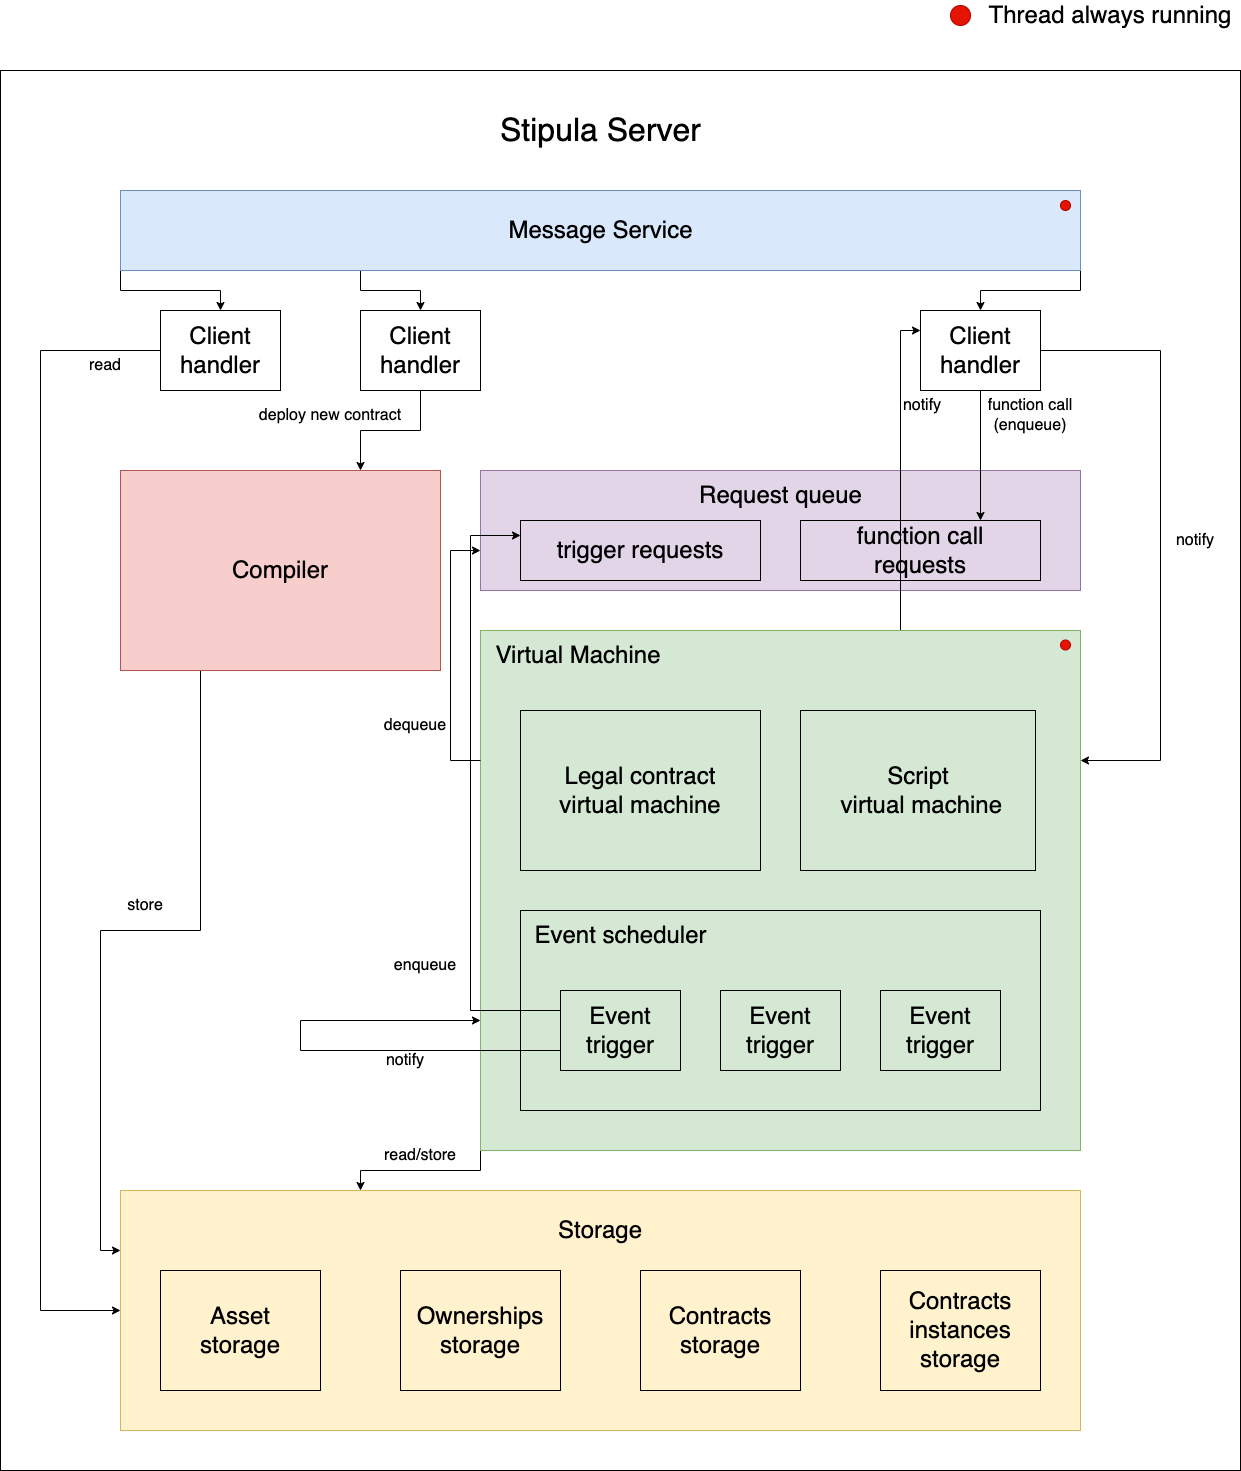
\includegraphics[width=0.9\textwidth]{immagini/capitolo-5/current-architecture.png}
		\caption{Current state of the implemented architecture.}
		\label{fig:current-architecture}
	\end{center}
\end{figure}

%**************************************************************

\section{Introduction to basic concepts}

The previous chapter introduced the concepts that form the basis on which the current architecture is 
based, such as assets and their management, and contracts. In this section these concepts will be analyzed 
from an implementation point of view, in order to help in understanding the functioning of the 
architecture in its complexity.

\subsection{Contracts and contract instances}
\label{contract-and-contract-instances-implementation}

In the current version of the architecture, there is a difference between a \textit{contract} and a 
\textit{instance of a contract}. The difference is similar to \textit{class} and \textit{object} (or 
\textit{instance of a class}) for object-oriented programming. When two actors want to \textit{execute} a 
contract, they will agree to create a new instance of a contract. The contract will be 
\textit{immutable}, while a contract instance can change over time.

From an implementation point of view, a contract is represented as follows:
\begin{enumerate}
  \item The source code of the contract;
  \item The compiled contract, that is, the bytecode;
  \item The initial state of the contract state machine;
  \item The final states of the contract state machine (optional);
  \item The contract state machine transitions.
\end{enumerate}

When this set of information is sent to the \textit{Storage} module, the latter generates an 
identification code to be associated with the contract. This identifier is sent in response to the client 
requesting to load the contract (see \ref{deploy-contract}). 

An instance of a contract is represented as follows:
\begin{enumerate}
   \item The \textbf{identifier of the contract}: it must be specified which specific contract you want 
   to refer to;
   \item The \textbf{participants of the contract};
   \item The definition of a \textbf{memory space} dedicated to maintaining the state of the global 
   variables during the evolution of the instance of the contract;
   \item A \textbf{state machine}: this structure is needed to track the progress of the contract 
   instance over time and to ensure that the contract participants operate without violating the 
   established order of operations.
\end{enumerate}

This distinction between contract and instance of a contract allows for the creation of multiple instances 
starting from the same contract, i.e., multiple users can use the same contract multiple times, present in 
a server or \textit{Stipula} node, creating multiple instances.

\subsection{Asset}

\subsubsection{Definition}
\label{asset-implementation}

As illustrated in the previous chapter (see \ref{asset-definition}), the goal is to try to reproduce the 
concept of \textit{token}, as is the case for Ethereum. An asset within the architecture is represented 
in Java by the object \verb|AssetConfig| class:
\begin{enumerate}
\item \verb|String assetName|: a name is defined that can be easily remembered by a person;
\item \verb|String unitName|: corresponds to what is a \textit{ticker} of a company listed on the stock 
exchange;
\item \verb|int decimals|: indicates how many parts a single unit can be in;
\item \verb|int supply|: indicates the maximum amount of assets that can exist over time.
\end{enumerate}

When this set of information is sent to the \textit{Storage} module, the latter generates an 
identification code to be associated with the asset. The object being stored contains the 
\verb|String id| fields and \verb|AssetConfig asset|.

At this point, creating \textit{fungible} and \textit{non-fungible} assets consists in extending the 
\verb|AssetConfig| class. In particular:
\begin{enumerate}
  \item 
  \begin{Verbatim}[numbers=left,xleftmargin=1cm,firstnumber=1,breaklines=true,breakanywhere=true,tabsize=2]
    public class FungibleAsset extends AssetConfig {
        public FungibleAsset(String assetName, String unitName, int supply, int decimals) {
            super(assetName, unitName, supply, decimals);
        }
    }
  \end{Verbatim}
  \item 
  \begin{Verbatim}[numbers=left,xleftmargin=1cm,firstnumber=1,breaklines=true,breakanywhere=true,tabsize=2]
    public class NonFungibleAsset extends AssetConfig {
        public NonFungibleAsset(String assetName, String unitName) {
            super(assetName, unitName, 1, 0);
        }
    }
  \end{Verbatim}
\end{enumerate}

\section{Libraries}
\label{libraries}

This package contains all the fundamental data structures for the overall development of the project. 
Furthermore, a library that implements cryptographic functions has been implemented.

\subsection{Crypto}

This library implements a number of cryptographic features, useful both for the architecture and for 
external software such as SDKs and wallets. The implemented methods are:
\begin{enumerate}
   \item \verb|generateKeyPair|: allows you to generate a 1024-bit RSA key pair;
   \item \verb|encrypt|: allows you to encrypt the received input;
   \item \verb|decrypt|: allows to decrypt the received input;
   \item \verb|getPublicKeyFromFile|: allows you to create a public key from a file;
   \item \verb|getPrivateKeyFromFile|: allows you to create a private key from a file;
   \item \verb|readKeyFromFile|: allows you to read a key from a file;
   \item \verb|getPublicKeyFromString|: allows you to create a public key from a string;
   \item \verb|sign|: allows you to sign the received input;
   \item \verb|verify|: allows you to verify if a signature is valid.
\end{enumerate}

\subsection{Data structures}

This package contains all the fundamental data structures for the implementation of the architecture. In 
particular, the data structures are:
\begin{enumerate}
   \item \verb|Pair|: represents a collection of two items of any type. The order of the elements is 
   important and allows two related values to be stored and manipulated as a single element;
   \item \verb|Triple|: it is a structure similar to the previous one, but it allows to manage three 
   elements;
   \item \verb|Queue|: is a data structure that implements the \textit{First-In-First-Out} 
   (\textit{FIFO}) policy, ie, the first item added to the queue is the first to be removed. This 
   structure is used when algorithms need to process a sequence of elements in a specific order;
   \item \verb|Stack|: is a data structure that implements the \textit{Last-In-First-Out} 
   (\textit{LIFO}) policy, i.e., the last element added to the stack is the first to be removed.
\end{enumerate}

In addition to these data structures, data structures provided directly by Java have been used, such as 
\textit{ArrayList} and \textit{HashMap}.

\section{Message Service}
\label{message-service}

This module is responsible for managing communication with clients, accepting their requests and 
redirecting them to the appropriate architecture modules. Before accepting requests, checks are carried 
out on the correct format of the message and the signatures associated with the message itself.

\subsection{MessageServer}

This component allows you to create an instance of a \textit{server}, which waits for new connections from 
\textit{clients}. When a new request arrives, the connection is delegated to a dedicated thread; by doing 
so, the server is ready to accept new connections. The other tasks of this component are to:
\begin{enumerate}
  \item Instruct the dedicated thread, passing it all the objects it needs;
  \item \label{shared-memory} Allocate a specific zone in \textbf{shared memory}. This memory zone is 
  shared between these threads and the virtual machine and is required for communication between these two 
  components. From the point of view of the implementation, shared memory is represented by one 
  \textit{map}, where the key is a string that serves as an identifier to access the cell, and the value 
  is a generic \verb|T| object.
\end{enumerate}

\subsection{ClientHandler}

This component takes care of managing a single connection with a client. In addition, this component takes 
care of:
\begin{enumerate}
   \item Check the \textit{signatures} of the message received from the client;
   \item If the previous check is successful, this component takes care of directing the request to the 
   correct module.
\end{enumerate}

When a response has been received from the module to which the request was directed, the 
\verb|ClientHandler| \textit{deallocate} the memory zone from shared memory.

\subsection{ClientConnection}

This component allows you to manage the connection more easily. In fact, it exposes high-level 
functionality, hiding certain complexities regarding socket management. This component allows you to make 
the \verb|ClientHandler| code more compact and readable.

\subsection{Messages}
\label{messages}

The messages currently in the implementation will be explained below. These represent the fundamental 
messages to allow the execution of the contracts. In the future, this ensemble will certainly be expanded. 
For ease of implementation, message transmission consists of direct encoding of Java objects in JSON 
format.

\subsubsection{DeployContract}
\label{deploy-contract}

This message allows you to load a new contract into the \textit{Stipula} instance. The only required value 
is the \textit{source code} of the contract. This request will then be routed to the compiler.

\subsubsection{FunctionCall}
\label{function-call-message}

This message allows you to make a function call for a specific instance of a contract. The required 
parameters are:
\begin{enumerate}
   \item \verb|contractInstanceId|: identifier of the instance of the contract to which it refers;
   \item \verb|functionName|: name of the function to call;
   \item \verb|arguments|: the list of arguments of the function to call. The elements of this list are 
   \textit{triples}. In this case, the meaning of a triple is \textit{variable type}, 
   \textit{variable name} and \textit{variable value}.
\end{enumerate}

This request will then be routed to the virtual machine.

\paragraph{Pay-to-Contract}
\label{pay-to-contract}

In the previous chapter the concept of \textit{Pay-to-Contract} was introduced (see 
\ref{pay-to-contract-and-pay-to-party}), that is, the user can make a payment to an instance of a 
contract, using one of its \textit{single-use-seals}. Previously, the \verb|FunctionCall| object was 
introduced, which allows you to supply the parameters of a specific function. These parameters are 
specified by the \verb|arguments| field, which is of type \verb|Triple<String, String, Object>|. The last 
component of the triple accepts a value of type \verb|String| or of type \verb|PayToContract|. This last 
object allows you to provide all the information necessary to make the payment to the contract instance. 
In particular, the fields of the object are:
\label{ownership}
\begin{enumerate}
   \item \verb|String ownershipId|: it is the identifier of the \textit{single-use-seal} that the user 
   wants to spend;
   \item \verb|String address|: the address of the owner of the \textit{single-use-seal};
   \item \verb|String unlockScript|: consists of a cryptographic proof proving that the user is the 
   effective owner of the \textit{single-use-seal}. The meaning of this field will be described later.
\end{enumerate}

Here is an example of \textit{Pay-to-Contract}:

\begin{Verbatim}[numbers=left,xleftmargin=1cm,firstnumber=1,breaklines=true,breakanywhere=true,tabsize=2]
  ...
  "arguments": [
    {
      "argument": {
        "first": "asset",
        "second": "y",
        "third": {
          "ownershipId": "2b4a4614-3bb4-4554-93fe-c034c3ba5a9c",
          "address": "ubL35Am7TimL5R4oMwm2OxgAYA3XT3BeeDE56oxqdLc=",
          "unlockScript": "PUSH str PLjodnT+m3RNIitQAPBDCsRmJPHCqrwZOY/CPiHFZGnl+DRN6soqxMy3ehTFaUwxBjjf7qfBfvTDq5oBItTFrtz1Rn5SDS1ybdbkwpKaOXVglNOw7ZEG9bbZ1mo1oA7IAjRiIilzUetCstE5rPZIf9XOXr/RQ5AHkZUn2CztsvA=\nPUSH str MIGfMA0GCSqGSIb3DQEBAQUAA4GNADCBiQKBgQCo/GjVKS+3gAA55+kko41yINdOcCLQMSBQyuTTkKHE1mhu/TgOpivM0wLPsSga8hQMr3+v3aR0IF/vfCRf6SdiXmWx/jflmEXtnT6fkGcnV6dGNUpHWXSpwUIDt0N88jfnEqekx4S+KDCKg99sGEeHeT65fKS8lB0gjHMt9AOriwIDAQAB\n"
        }
      }
    }
  ],
  ...
\end{Verbatim}

\subsubsection{AgreementCall}
\label{agreement-call-message}

The \textit{agreement} function is a particular function compared to the others and therefore must be 
managed ad-hoc. For this function you need:
\begin{enumerate}
  \item \verb|contractId|: identifier of the contract. This function call will create a 
  \textit{new instance of the indicated contract};
  \item \verb|arguments|: the list of arguments of the function to call;
  \item \verb|parties|: is a map that provides the association between the party name in the contract 
  and the user's \textit{address} and \textit{public key}. An address is a compact representation of the 
  public key, in particular, it is the hash of the public key. For example:
  \begin{Verbatim}[numbers=left,xleftmargin=1cm,firstnumber=1,breaklines=true,breakanywhere=true,tabsize=2]
    ...
    "parties": {
      "Bob": {
        "address": "f3hVW1Amltnqe3KvOT00eT7AU23FAUKdgmCluZB+nss=",
        "publicKey": "MIGfMA0GCSqGSIb3DQEBAQUAA4GNADCBiQKBgQDErzzgD2ZslZxciFAiX3/ot7lrkZDw4148jFZrsDZPE6CVs9xXFSHGgy/mFvIFLXhnChO6Nyd2be3lbgeavLMCMVUiTStXr117Km17keWpb3sItkKKsLFBOcIIU8XXowI/OhzQN2XPZYESHgjdQ5vwEj2YyueiS7WKP94YWz/pswIDAQAB"
      },
      "Alice": {
        "address": "ubL35Am7TimL5R4oMwm2OxgAYA3XT3BeeDE56oxqdLc=",
        "publicKey": "MIGfMA0GCSqGSIb3DQEBAQUAA4GNADCBiQKBgQCo/GjVKS+3gAA55+kko41yINdOcCLQMSBQyuTTkKHE1mhu/TgOpivM0wLPsSga8hQMr3+v3aR0IF/vfCRf6SdiXmWx/jflmEXtnT6fkGcnV6dGNUpHWXSpwUIDt0N88jfnEqekx4S+KDCKg99sGEeHeT65fKS8lB0gjHMt9AOriwIDAQAB"
      }
    },
    ...
  \end{Verbatim}
  
  \verb|Alice| and \verb|Bob| are the names of the variables representing the parties in the contract. 
  With this function call, these variables now have an associated address and public key.

  The \verb|AgreementCall| is a bit more complicated than just \verb|FunctionCall|. The reason is that in 
  order to agree to a contract, both parties to the contract must sign a \textbf{single message}. There 
  are different ways to collect signatures to add to your message. An easy way could be for the two 
  parties to the contract to agree on the terms of a contract (i.e., the cost of a service) by means of 
  communication channels such as chat or email. One of the two parties creates the \verb|AgreementCall| 
  message, signs it with his private key and sends it via chat or email to the other party. The other 
  party downloads the message, checks that the previously agreed values have been entered, checks that 
  the other party's signature is legitimate and also signs the message. Once this procedure has been 
  carried out, one of the two actors sends the \verb|AgreementCall| message \textit{only once} to the 
  server. Another context could be an external application that relies on a \textit{Stipula server}. This 
  application can perform the same operations described in the previous example, hiding all the steps 
  through a single graphical interface. Once all the signatures of the actors have been collected, the 
  application, based on the \textit{Stipula server}, will send the \verb|AgreementCall| to the 
  \textit{Stipula server}. The advantage of having structured the architecture and the communication in 
  this way is that it does not place any constraints on the communication between the actors. When the 
  \textit{Stipula server} has received the \verb|AgreementCall| message with legitimate signatures, the 
  architecture will create a new instance of the contract chosen by the actors.

  The \verb|AgreementCall| request it will then be directed to the virtual machine.
\end{enumerate}

\subsubsection{GetAssetById}

This message allows you to obtain information about a specific asset, given an identifier. In fact, the 
only required value is the \textit{identifier of the asset} whose information is to be obtained.

This request will then be routed to \textit{Storage}.

\subsubsection{GetOwnershipsByAddress}

This message allows you to get all spent and unspent funds from a specific address. In fact, the only 
required value is a \verb|address|. The use of an address allows to transmit less data in the socket and 
to carry out less computations in the \textit{Storage} to find the address associated with the public key.

This request will then be routed to \textit{Storage}.

\subsection{Interaction with Storage}

The only requests that allow this module to interact \textit{directly} with the \textit{Storage} module 
are \verb|GetAssetById| and \verb|GetOwnershipsByAddress|. These messages require to be able to obtain 
information, that is, to perform a \textit{read} operation from the \textit{Storage} module. In fact, all 
the requests that imply a modification of a piece of information are requests that are addressed to the 
compiler and virtual machine modules. Only these two modules can actually \textit{write} to 
\textit{Storage}.

\section{Compiler}
\label{compiler}

A \textit{compiler} is a software program that translates source code, written in a high-level programming 
language, into machine code that can be executed by a computer. In this case, we want to develop a 
compiler to translate the high-level language \textit{Stipula} into a language that can be executed by a 
machine: the \textit{Stipula bytecode}.

A compiler is made up of several components, which can be grouped into:
\begin{enumerate}
  \item \textbf{Front-end}: it is the part of the compiler that deals directly with the source code and 
  produces an internal representation that can be easily processed by the back-end. The front-end output 
  is usually an intermediate representation such as an \textit{abstract syntax tree}, which can be 
  optimized and transformed by the back-end before being translated into machine code or some other target 
  language. This involves tasks such as \textit{lexical parsing} (splitting input into tokens), 
  \textit{syntax parsing} (parsing tokens into a parse tree or an abstract syntax tree), and 
  \textit{semantic analysis} (making sure the input conforms to the rules of the language and generating 
  an intermediate representation);
  \item \textbf{Back-end}: is responsible for generating executable code from the intermediate 
  representation produced by the front-end. This involves several stages, including:
  \begin{enumerate}
    \item \textit{Optimization}: this phase involves the analysis of the intermediate code and its 
    transformation to produce a more efficient code;
    \item \textit{Code generation}: in this phase, the optimized intermediate code is transformed into 
    executable machine code. This involves translating each intermediate code instruction into one or more 
    machine instructions, taking into account the target hardware platform and processor specific 
    instruction set;
    \item \textit{Linking}: The generated code is combined with any required runtime libraries and other 
    resources to produce an executable program.
  \end{enumerate}
  A compiler's backend is typically heavily dependent on the target architecture, and different backends 
  may be needed for different hardware platforms or operating systems.
\end{enumerate}

The typical structure of a compiler includes the following components:
\begin{enumerate}
  \item \textbf{Lexer}: this component reads the source code character by character and decomposes it into 
  \textit{token}. A token is a sequence of characters that represents a significant unit of the language, 
  such as a keyword, an identifier or an operator;
  \item \textbf{Parser}: this component takes the stream of tokens generated by the lexer and builds a 
  \textbf{syntax tree} or an \textbf{abstract syntax tree} (\textbf{AST}) which represents the syntax 
  structure of the program. The AST captures the hierarchical relationships between language constructs in 
  the program;
  \item \textbf{Semantic Analyzer}: This component checks the AST for semantic correctness, such as type 
  checking and error detection. Ensures that the program follows the rules of the programming language and 
  can run correctly;
  \item \textbf{Intermediate code generator}: this component translates the AST into an intermediate 
  representation, i.e. a machine-independent low-level code that can be optimized and further translated 
  into executable code;
  \item \textbf{Code optimizer}: this component applies various optimization techniques to intermediate 
  code to improve its efficiency and reduce its size;
  \item \textbf{Code generator}: this component translates the optimized intermediate code into machine 
  code that can be executed by the target processor;
  \item \textbf{Linker}: this component combines the object files produced by the code generator into a 
  single executable file and resolves any external references between them.
\end{enumerate}

An external tool (see section \ref{lexer-parser-antlr}) was used to automate the development of some parts 
of the compiler. The part that was implemented manually is the part that concerns the \textit{mapping} of 
the \textit{Stipula} instructions into \textit{Stipula bytecode} instructions.

For the implementation of the compiler not all the steps described have been followed:
\begin{enumerate}
  \item The \textit{linker} is not useful in the current state of the language;
  \item The \textit{intermediate code generator} is replaced by the \textit{code generator}, as the 
  \textit{Stipula bytecode} already represents the target language;
  \item The \textit{code optimization} phase is missing, especially when it comes to analyzing and solving 
  \textit{syntactic sugar}. In particular, see \ref{syntactic-sugar} for an illustration of this problem.
\end{enumerate}

\subsection{Grammar, lexer e parser}

\subsubsection{Grammar}
\label{grammar}

The original grammar of the \textit{Stipula} language (\cite{site:stipula-java-centralized-grammar} and 
\cite{site:stipula-java-centralized-syntax}) is as follows:
{
  \small
  \\
  \noindent
  <\textit{prog}> ::= \verb|'stipula'| <\textit{id}> '\verb|{|' <\textit{declist}>$^*$ <\textit{agreement}>? <\textit{fun}>+ '\verb|}|';
  \\\\
  \noindent
  <\textit{agreement}> ::= (\verb|'agreement'| '\verb|(|' <\textit{disputer}> (\verb|','| <\textit{disputer}>)$^*$ '\verb|)|' '\verb|(|' <\textit{vardec}> ('\verb|,|' <\textit{vardec}>)$^*$ '\verb|)|' '\verb|{|' (<\textit{assign}>)+ '\verb|}|' '\verb|==>|' '\verb|@|' <\textit{state}>);
  \\\\
  \noindent
  <\textit{fun}> ::= (('\verb|@|' <\textit{state}>)+ <\textit{disputer}> ('\verb|,|' <\textit{disputer}>)$^*$ '\verb|:|' <\textit{id}> '\verb|(|' (<\textit{vardec}> ('\verb|,|' <\textit{vardec}>)$^*$)? '\verb|)|' '\verb|[|' (<\textit{assetdec}> ('\verb|,|' <\textit{assetdec}>)$^*$)? '\verb|]|' ('\verb|(|' <\textit{prec}> '\verb|)|')? '\verb|{|' <\textit{stat}>+ '\verb|;|' <\textit{events}>+ '\verb|}|' '\verb|==>|' '\verb|@|' <\textit{state}>);
  \\\\
  \noindent
  <\textit{assign}> ::= (<\textit{disputer}> ('\verb|,|' <\textit{disputer}>)$^*$ '\verb|:|' <\textit{vardec}> ('\verb|,|' <\textit{vardec}>)$^*$);
  \\\\
  \noindent
  <\textit{stat}> ::= '\verb|_|' | (<\textit{value}> ('\verb|->|' | '\verb|-o|') <\textit{value}> ('\verb|,|' <\textit{value}>)?) | <\textit{ifelse}>;
  \\\\
  \noindent
  <\textit{ifelse}> ::= ('\verb|if|' '\verb|(|' <\textit{expr}> '\verb|)|' '\verb|{|' <\textit{stat}>+ '\verb|}|' ('\verb|else if|' '\verb|(|' <\textit{expr}> '\verb|)|' '\verb|{|' <\textit{stat}>+ '\verb|}|')$^*$ ('\verb|else|' '\verb|{|' <\textit{stat}>+ '\verb|}|')?);
  \\\\
  \noindent
  <\textit{events}> ::= '\verb|_|' | (<\textit{expr}> '\verb|>>|' '\verb|@|' '\verb|id|' '\verb|{|' <\textit{stat}>+ '\verb|}|' '\verb|==>|' '\verb|@|' '\verb|id|');
  \\\\
  \noindent
  <\textit{prec}> ::= <\textit{expr}>;
  \\\\
  \noindent
  <\textit{expr}> ::= ('\verb|-|')? <\textit{term}> (('\verb|+|' | '\verb|-|' | '\verb||||') <\textit{expr}>)?;
  \\\\
  \noindent
  <\textit{term}> ::= <\textit{factor}> (('\verb|*|' | '\verb|/|' || '\verb|&&|') <\textit{term}>)?;
  \\\\
  \noindent
  <\textit{factor}> ::= <\textit{value}> (('\verb|==|' | '\verb|<|' | '\verb|>|' | '\verb|<=|' | '\verb|>=|' | '\verb|!=|') <\textit{value}>)?;
  \\\\
  \noindent
  <\textit{varasm}> ::= <\textit{vardec}> '\verb|=|' <\textit{expr}>;
  \\\\
  \noindent
  <\textit{declist}> ::= <\textit{type}> <\textit{strings}>;
  \\\\
  \noindent
  <\textit{type}> ::= '\verb|asset|' | '\verb|field|' | '\verb|int|' | '\verb|real|' | '\verb|boolean|' | '\verb|party|' | '\verb|string|' | '\verb|time|' | '\verb|init|';
  \\\\
  \noindent
  <\textit{state}> ::= <\textit{strings}>;
  \\\\
  \noindent
  <\textit{disputer}> ::= <\textit{strings}>;
  \\\\
  \noindent
  <\textit{vardec}> ::= <\textit{strings}>;
  \\\\
  \noindent
  <\textit{assetdec}> ::= <\textit{strings}>;
  \\\\
  \noindent
  <\textit{value}> ::= <\textit{number}> | '\verb|now|' | '\verb|(|' <\textit{expr}> '\verb|)|' | <\textit{strings}> | '\verb|_|' | ('\verb|true|' | '\verb|false|');
  \\\\
  \noindent
  <\textit{id}> ::= '\verb|id|';
  \\\\
  \noindent
  <\textit{strings}> ::= \verb|SINGLE_STRING| | \verb|DOUBLE_STRING| | '\verb|id|';
  \\\\
  \noindent
  <\textit{real}> ::= <\textit{number}> '\verb|.|' <\textit{number}>;
  \\\\
  \noindent
  <\textit{number}> ::= \verb|INT| | \verb|REAL|;
  \\
}

This grammar has a limitation regarding assets. Suppose you need to write a contract to swap two assets. 
The code could be as follows:

\begin{Verbatim}[numbers=left,xleftmargin=1cm,firstnumber=1,breaklines=true,tabsize=2]
  stipula SwapAsset {
    asset assetA, assetB
    field amountAssetA, amountAssetB
    ...
\end{Verbatim}

However, from this code it is not possible to understand which assets are being referred to exactly. That 
is, if Alice wants to swap \textit{assetA} for \textit{assetB} owned by Bob, there is no specific 
indication of these assets in the code. The change that was made to the grammar is as follows:
\\\\
\noindent
<\textit{declist}> ::= (<\textit{assetdecl}>)? (<\textit{fielddecl}>)?;
\\\\
\noindent
<\textit{assetdecl}> ::= '\verb|asset|' <\textit{strings}> '\verb|:|' <\textit{strings}>;
\\\\
\noindent
<\textit{fielddecl}> ::= <\textit{type}> <\textit{strings}>;
\\\\
\noindent
<\textit{type}> ::= '\verb|field|' | '\verb|int|' | '\verb|real|' | '\verb|boolean|' | '\verb|party|' | '\verb|string|' | '\verb|time|' | '\verb|init|';
\\

By doing so, it is possible to specify the assets that must be accepted by the contract. Thus, the 
previous code in \textit{Stipula} transforms with the grammar change as follows:

\begin{Verbatim}[numbers=left,xleftmargin=1cm,firstnumber=1,breaklines=true,tabsize=2]
  stipula SwapAsset {
    asset assetA:stipula_assetA_ed8i9wk, assetB:stipula_assetB_pl1n5cc
    field amountAssetA, amountAssetB
    ...
\end{Verbatim}

The \ref{app:grammar} appendix illustrates the rules of the defined grammar previously (see \ref{grammar}) 
translated into \textbf{ANTLR}. 

\subsubsection{Lexer, Parser and ANTLR}
\label{lexer-parser-antlr}

\textit{ANTLR} (\textit{ANother Tool for Language Recognition}) is a \textbf{lexer} and \textbf{parser} 
generator that can be used to create compilers, interpreters and other language processing tools. It is a 
tool well known for its ability to generate highly efficient parsers that can handle complex and context 
sensitive grammars. It also provides a simple syntax for defining grammars, which makes it easier to 
create parsers for new languages or formats.

In order to use this tool, it is necessary to convert the grammar defined in the previous section, 
following the rules established by ANTLR (see the \ref{app:grammar} appendix). Version 4.10 was used for 
this project \autocite{site:antlr-version}. 

The tool is written in Java and in order to use it you need to execute a \verb|.jar| file. In particular, 
the command to generate the classes that implement the lexer and the parser is the following:
\begin{Verbatim}
  java -jar antlr-4.10-complete.jar -visitor Stipula.g4
\end{Verbatim}

In order to use the lexer and parser produced by ANTLR, it is necessary to integrate the latter tool into 
the project. The integration is specified in the \ref{app:gradle} appendix.

\subsection{Generation of the bytecode}

This stage occurs after the parser has produced the abstract syntax tree. In particular, the AST is 
visited and for each instruction of the \textit{Stipula} language one or more bytecode instructions are 
generated. In this phase, any syntactic sugar present in the contract is also resolved. The translation 
of the syntactic sugar takes place by generating fixed structures in bytecode language, that is, once the 
syntax variant of a specific instruction has been recognized, this is always translated into a fixed 
structure. This practice allows in the execution phase not to worry about the presence of any syntactic 
sugar to be resolved.

Once compiled, the source code of the contract and the compiled are stored in the \textit{Storage} module.

In the next section we will introduce the \textit{Stipula bytecode} language, that is, its functioning and 
its instructions.

\section{Stipula bytecode}
\label{stipula-bytecode}

This language was designed to mirror the functionality of the high-level language and to run on a 
\textit{stack-based} virtual machine. A summary table of the instructions is shown below 
\ref{table:bytecode-instructions}: the \verb|-| symbol means that the statement takes no value as input 
or returns no value as output, while the \verb|*| means that the instruction accepts a value of any type 
or outputs a value of any type.

\begin{ThreePartTable}
  \begin{longtable}{|c|c|}
    \caption{Table of \textit{Stipula bytecode} instructions.}
    \label{table:bytecode-instructions}\\
    \noalign{\global\arrayrulewidth0.7pt}
    \hline
    \textbf{Instruction} & \textbf{Behavior} \\ [5pt]
    
    \noalign{\global\arrayrulewidth0.7pt}
    \hline
    
    \verb|PUSH|     & $- \rightarrow *$ \\
    \hline
    
    \verb|HALT|     & $- \rightarrow -$ \\
    \hline

    \verb|ADD|      & $(\verb|int|, \verb|int|) \rightarrow \verb|int|$,      \\
                    & $(\verb|real|, \verb|real|) \rightarrow \verb|real|$,   \\
                    & $(\verb|asset|, \verb|asset|) \rightarrow \verb|real|$, \\
                    & $(\verb|asset|, \verb|real|) \rightarrow \verb|real|$,  \\
                    & $(\verb|real|, \verb|asset|) \rightarrow \verb|real|$,  \\
                    & $(\verb|time|, \verb|time|) \rightarrow \verb|time|$    \\
    \hline

    \verb|SUB|      & $(\verb|int|, \verb|int|) \rightarrow \verb|int|$,      \\
                    & $(\verb|real|, \verb|real|) \rightarrow \verb|real|$,   \\
                    & $(\verb|asset|, \verb|asset|) \rightarrow \verb|real|$, \\
                    & $(\verb|asset|, \verb|real|) \rightarrow \verb|real|$,  \\
                    & $(\verb|real|, \verb|asset|) \rightarrow \verb|real|$   \\
    \hline
    
    \verb|MUL|      & $(\verb|int|, \verb|int|) \rightarrow \verb|int|$,      \\
                    & $(\verb|real|, \verb|real|) \rightarrow \verb|real|$,   \\
                    & $(\verb|asset|, \verb|asset|) \rightarrow \verb|real|$, \\
                    & $(\verb|asset|, \verb|real|) \rightarrow \verb|real|$,  \\
                    & $(\verb|real|, \verb|asset|) \rightarrow \verb|real|$   \\
    \hline
    
    \verb|DIV|      & $(\verb|int|, \verb|int|) \rightarrow \verb|int|$,      \\
                    & $(\verb|real|, \verb|real|) \rightarrow \verb|real|$,   \\
                    & $(\verb|asset|, \verb|asset|) \rightarrow \verb|real|$, \\
                    & $(\verb|asset|, \verb|real|) \rightarrow \verb|real|$,  \\
                    & $(\verb|real|, \verb|asset|) \rightarrow \verb|real|$   \\
    \hline
    
    \verb|INST|     & $- \rightarrow -$ \\
    \hline

    \verb|AINST|    & $- \rightarrow -$ \\
    \hline

    \verb|GINST|    & $- \rightarrow -$ \\
    \hline
    
    \verb|LOAD|     & $- \rightarrow *$ \\
    \hline

    \verb|ALOAD|    & $- \rightarrow *$ \\
    \hline

    \verb|GLOAD|    & $- \rightarrow *$ \\
    \hline
    
    \verb|STORE|    & $* \rightarrow -$ \\
    \hline

    \verb|ASTORE|   & $* \rightarrow -$ \\
    \hline

    \verb|GSTORE|   & $* \rightarrow -$ \\
    \hline
    
    \verb|AND|      & $(\verb|bool|, \verb|bool|) \rightarrow \verb|bool|$ \\
    \hline
    
    \verb|OR|       & $(\verb|bool|, \verb|bool|) \rightarrow \verb|bool|$ \\
    \hline
    
    \verb|NOT|      & $\verb|bool| \rightarrow \verb|bool|$ \\
    \hline
    
    \verb|JMP|      & $- \rightarrow -$ \\
    \hline

    \verb|JMPIF|    & $\verb|bool| \rightarrow -  \text{ || } \verb|bool|$ \\
    \hline

    \verb|ISEQ|     & $* \rightarrow \verb|bool|$ \\
    \hline

    \verb|ISLE|     & $* \rightarrow \verb|bool|$ \\
    \hline

    \verb|ISLT|     & $* \rightarrow \verb|bool|$ \\
    \hline

    \verb|DEPOSIT|  & $(\verb|asset|, \verb|asset|) \rightarrow -$ \\
    \hline

    \verb|WITHDRAW| & $(\verb|real|, \verb|asset|, \verb|party|) \rightarrow -$ \\
    \hline

    \verb|RAISE|    & $- \rightarrow \verb|str|$ \\
    \hline

    \verb|TRIGGER|  & $\verb|time| \rightarrow -$ \\
    
    \noalign{\global\arrayrulewidth0.7pt}
    \hline
  \end{longtable}
\end{ThreePartTable}

\subsection{Types}

This section introduces the types that are supported by the \textit{Stipula bytecode}.

\paragraph{Integers, Strings e Booleans}

These are the simplest types to implement, as only one field in the Java object representation is 
required for storing the value. Examples of declarations:
\begin{enumerate}
  \item Integer: \verb|int <variable_name> 123|;
  \item String: \verb|str <variable_name> abc|;
  \item Boolean: \verb|bool <variable_name> true| or \verb|bool <variable_name> false|.
\end{enumerate}

\paragraph{Time}

From an implementation point of view, this type is similar to the previous one. However, the value of a 
variable of type \verb|time| represents a certain amount of time expressed in \textit{seconds}. Example 
of declaration: \verb|time <variable_name> 123|.

\paragraph{Real numbers}

This type was implemented in a simple way: there are two fields, one representing the number for 
\textit{extended}, that is, without the comma; the other indicates the \textit{number of decimals} to 
apply to the number contained in the first field. For example, to encode the number $134.28$ you would 
write $13428 \text{ } 2$, that is, $13428$ represents the number in full and $2$ represents the number of 
decimals to apply to that value. Example of declaration: \verb|float <variable_name> 123 1| means $12.3$.

\paragraph{Party}
\label{party-implementation}

The Java object that represent the type \verb|party| in the bytecode language is structured as follows:
\begin{Verbatim}[numbers=left,xleftmargin=1cm,firstnumber=9,breaklines=true,breakanywhere=true,tabsize=2]
  ...
  public class Party implements Serializable {
    private final String address;
    private final String publicKey;

    public Party(String publicKey) throws NoSuchAlgorithmException {
        this.publicKey = publicKey;

        // Hash the public key
        Base64.Encoder encoder = Base64.getEncoder();
        MessageDigest digest = MessageDigest.getInstance("SHA-256");

        this.address = encoder.encodeToString(digest.digest(publicKey.getBytes(StandardCharsets.UTF_8)));
    }
  ...
\end{Verbatim}
\begin{enumerate}
  \item \verb|publicKey| represents a user's public key;
  \item \verb|address| is a more compact representation of the public key, in particular, it is the 
  \textit{hash} of the public key. Having this field will allow you to use less space and make 
  \textit{Storage} searches faster.
\end{enumerate}

Example of declaration: 
\begin{Verbatim}[xleftmargin=1cm,breaklines=true,breakanywhere=true,tabsize=2]
  party <variable_name> ubL35Am7TimL5R4oMwm2OxgAYA3XT3BeeDE56oxqdLc=
\end{Verbatim}

\paragraph{Asset}

The structure of this type consists of:
\begin{enumerate}
   \item The \verb|real| part represents the quantity of assets contained in the variable;
   \item The \verb|assetId| field represents the identifier of the asset. This makes it possible to 
   understand which asset the quantity specified by the real part belongs to.
\end{enumerate}

Example of declaration: \verb|asset <variable_name> 100 2 stipula_coin_asd345|.

\subsection{Instructions of the bytecode language}

In this section we will explain how the language instructions work. In section \ref{stack-based-vm} it 
was explained what a stack-based virtual machine is. The virtual machine is able to manage the values 
on the stack by means of two operations. When an instruction takes a value as input, it means that it 
\textit{pop} from the stack. While, when an instruction returns a value in output, it means that it 
performs the \textit{push} operation on the stack.

\paragraph{PUSH}

This statement allows you to insert values into the \textit{stack}. This statement takes an input value 
of any type and returns no output value. Possible formats for this statement are:
\begin{enumerate}
  \item \verb|PUSH int <value>|;
  \item \verb|PUSH bool <value>|;
  \item \verb|PUSH str <value>|;
  \item \verb|PUSH party <value>|;
  \item \verb|PUSH time <value>| and \verb|PUSH time now|: \verb|now| is a reserved word and 
  when this instruction is read by the virtual machine, this word is interpreted as the 
  intention to get the current \textit{timestamp};
  \item \verb|PUSH real <value> <decimals>| (i.e., \verb|PUSH real 13428 2|);
  \item \verb|PUSH asset <value> <decimals> <asset-id>|\\ 
  (i.e., \verb|PUSH asset 13428 2 stipulation_coin_asd345|).
\end{enumerate}

\paragraph{HALT}

This statement notifies the virtual machine that the function code is finished. If this statement is 
executed, it means that the entire execution of the function did not generate any errors. With this 
instruction, the virtual machine proceeds to store the results produced, send any payments to addresses 
and provide a response for the client. This statement takes no value as input and returns no output.

\paragraph{ADD}

This statement implements the \textit{sum} mathematical operation. This statement takes two values as 
input and returns one value as output. In most cases, the types of the two input values must be equal to 
each other, and the type of the output value must be equal to the type of the input values. For example, 
if two values of type \verb|int| are received as input, then the output will be of type \verb|int|.

However, there is an exception regarding the \verb|asset| type. In fact, manipulation of variables of this 
type must be done with great caution. If you want to somehow add the amount of assets owned by a specific 
instance of a contract with other values, this operation must absolutely not affect the amount of assets 
present, that is, a sum operation involving a variable of type \verb |asset|, must ensure that after this 
operation no quantity has been lost or some quantity of asset has been generated out of thin air. The only 
operations that can manipulate the quantity of assets contained in the appropriate variable are the 
\textit{deposit} and \textit{withdrawal} operations, which will be described later. Therefore, the 
application of mathematical operations to variables of type \verb|asset| has been limited as follows:
\begin{enumerate}
  \item A variable of type \verb|real| is accepted as input and one of type \verb|asset| and the output 
  of the operation will be a value of type \verb|real|;
  \item A variable of type \verb|asset| is accepted as input and one of type \verb|real| and the output 
  of the operation will be a value of type \verb|real|;
\end{enumerate}

By doing so, it is not possible to generate or destroy quantities of assets through the use of 
mathematical operations.

Finally, this is the only mathematical instruction that allows you to manipulate \verb|time| values. 
Therefore, this sequence of instructions:
\begin{Verbatim}[numbers=left,xleftmargin=1cm,firstnumber=1,tabsize=2]
  ...
  GLOAD waitTime
  PUSH time now
  ADD
  ...
\end{Verbatim}

will add the value contained in the global variable \verb|waitTime| at the \textit{timestamp} calculated 
at the instant in which the virtual machine will read the instruction on line 3.

\paragraph{SUB, MUL and DIV}

These instructions implement the mathematical operations of \textit{subtraction}, \textit{multiplication} 
and \textit{division}, respectively. The behavior of these instructions is similar to the operation of the 
add instruction, except that they cannot handle values of type \verb|time|.

\paragraph{INST, AINST and GINST}

These statements take no value as input and return no value as output. These statements allow you to 
\textit{instantiate} new variables. In particular:
\begin{enumerate}
  \item \verb|INST| allows to instantiate a variable in the space dedicated to the function;
  \item \verb|AINST| allows you to instantiate a variable in the space dedicated to the function's 
  arguments;
  \item \verb|GINST| allows you to instantiate a variable in the space dedicated to global variables of 
  the contract instance.
\end{enumerate}

The possible formats for these instructions are:
\begin{enumerate}
  \item \verb|INST | AINST | GINST <int | bool | str | party | time> <value>|;
  \item \verb|INST | AINST | GINST time <value> | now|;
  \item \verb|INST | AINST | GINST real <value> <decimals>|;
  \item \verb|INST | AINST | GINST asset <value> <decimals> <asset-id>|;
  \item \verb|INST | AINST | GINST * <value>|: this format allows you to instantiate a variable whose 
  type must be determined at runtime.
\end{enumerate} 

Before instantiating a new variable, the virtual machine will make sure that another variable with the 
same name does not exist in memory.

\paragraph{LOAD, ALOAD and GLOAD}

These instructions allow you to \textit{load} a variable from memory onto the stack. These instructions 
take no value as input and return the variable loaded from memory as output. In particular:
\begin{enumerate}
  \item \verb|LOAD|: allows you to load a variable from the space dedicated to the function;
  \item \verb|ALOAD|: allows you to load a variable from the space dedicated to the function arguments;
  \item \verb|GLOAD|: allows you to load a variable from the space dedicated to global variables of the 
  contract instance.
\end{enumerate}

The instruction formats are:
\begin{Verbatim}
  LOAD | ALOAD | GLOAD <variable_name>
\end{Verbatim}

Before loading a variable, the virtual machine will make sure that the variable exists in memory.

\paragraph{STORE, ASTORE and GSTORE}

These statements allow you to \textit{store} a variable in memory. These statements take a value of any 
type as input and return no value as output. In particular:
\begin{enumerate}
   \item \verb|STORE|: allows you to store a variable in the space dedicated to the function;
   \item \verb|ASTORE|: allows you to store a variable in the space dedicated to the function arguments;
   \item \verb|GSTORE|: allows you to store a variable in the space dedicated to the global variables of 
   the contract instance.
\end{enumerate}

The instruction formats are:
\begin{Verbatim}
  STORE | ASTORE | GSTORE <variable_name>
\end{Verbatim}

Before storing the variable, the virtual machine will make sure that the variable exists in memory.

\paragraph{AND and OR}

These statements take two \textit{boolean} values as input and return a boolean value as output. For the 
\verb|AND| statement, if both input values are \verb|true|, then the output will be \verb|true|, otherwise 
the output will be \verb|false|. While, for the \verb|OR| statement, if one of the two input values is 
\verb|true|, then the output will be \verb|true|, otherwise the output will be \verb|false|.

\paragraph{NOT}

This statement takes a \textit{boolean} value as input and returns a boolean value as output. The output 
of this statement is the inverse of the input value, that is, if the input is \verb|true|, then the output 
will be \verb|false|, and vice versa.

\paragraph{ISEQ}

Given two boolean inputs, this statement checks whether two values are \textit{equal}. If the input values 
are equal, the output will be \verb|true|, otherwise the output will be \verb|false|. This statement can 
be applied to any type, as long as the input types are the same. The only allowed exceptions are the input 
pairs (\verb|asset|, \verb|real|) and (\verb|real|, \verb|asset|).

Combining this statement with the \verb|NOT| statement it is possible to check if the two input values are 
different from each other: if the values are \textit{different}, the output will be \verb|true|, otherwise 
the output will be \verb|false|.

\paragraph{ISLE}

Given two boolean inputs, this statement checks whether the first value is \textit{less than or equal} to 
the second value. If this condition is true, then the output will be \verb|true|, otherwise the output 
will be \verb|false|. This statement only applies to types \verb|int|, \verb|real| and \verb|assets|.

Combining this statement with the \verb|NOT| statement it is possible to check if the first value is 
\textit{strictly greater} than the second value: if this condition is true, the output will be 
\verb|true|, otherwise the output will be \verb|false|.

\paragraph{ISLT}

Given two boolean inputs, this statement checks whether the first value is \textit{strictly less} than the 
second value. If this condition is true, then the output will be \verb|true|, otherwise the output will be 
\verb|false|. This statement only applies to types \verb|int|, \verb|real| and \verb|assets|.

Combining this statement with the \verb|NOT| statement it is possible to check if the first value is 
\textit{greater than or equal} to the second value: if this condition is true, the output will be 
\verb|true|, otherwise the output will be \verb|false|.

\paragraph{JMP}

This statement takes no value as input and returns no value as output. This instruction represents the 
\textit{unconditional jump} and allows interrupting the normal flow of execution of the function to reach 
a specific area of code (always within the function), indicated by a \textit{label}. The format of the 
statement is \verb|JMP <label>|. Since the high-level language \textit{Stipula} is not a Turing complete 
language, it is not possible to create loops with this instruction, since the jump can only be made in 
\textit{"forward"}, i.e., the search of the \textit{label} starts from the position where the last 
statement was just executed and goes forward, it is not allowed to search for the label starting from the 
beginning of the function. 

\paragraph{JMPIF}

This instruction takes as input a value of type \verb|bool|. This instruction allows to implement the 
\textit{conditional jump}, that is, it is possible to interrupt the normal execution flow and reach a 
specific area of code, within the function, only if a previous condition has been satisfied. The format 
of the statement is \verb|JMPIF <label>|. If the input value is \verb|true|, then jumping to the code area 
indicated by \verb|<label>| will happen and no value will be output, otherwise if the input value is 
\verb|false|, the input value will be output.

\paragraph{DEPOSIT}

This statement takes two values as input, both of type \verb|asset|, and returns no value as output. This 
statement allows you to \textit{deposit} assets into an instance of a contract. The first value represents 
the amount of assets deposited by the user and this amount is \textit{accumulated} into the second value, 
which represents the amount of assets present in the contract instance. This is one of two instructions 
that is allowed to directly manage assets and store updates to these variables.

\paragraph{WITHDRAW}

This instruction allows you to make payments to a specific participant of the contract. This statement 
takes three values as input and returns no value as output. The input values are:
\begin{enumerate}
  \item \verb|real|: this value represents the quantity of assets that must be withdrawn;
  \item \verb|asset|: this value represents the quantity of assets contained in the contract instance;
  \item \verb|party|: this value represents the party of the contract to which the payment must be made.
\end{enumerate}

This instruction is allowed to directly manage the assets and to store the updates regarding these 
variables.

\paragraph{RAISE}

This statement takes no value as input and outputs a value of type \verb|str| which will be placed on the 
\textit{error stack} of the virtual machine. This statement is used to block the flow of function 
execution to notify an error. In this version of the architecture, the only error that can be reported to 
the error stack is \verb|AMOUNT_NOT_EQUAL| and is notified when the user wants to deposit an amount of 
assets that does not match the amount of assets agreed at the beginning of the contract.

\paragraph{TRIGGER}

This instruction takes as input a value of type \verb|time| and returns no output. This instruction allows 
you to create an event to schedule, at a precise moment, the execution of a \textit{obligation}. The 
format of the instruction is \verb|TRIGGER <obligation_function_name>|, having to for 
\verb|<obligation_function_name>| we refer to the name of the function that encodes the obligation that 
will have to be performed.

\subsection{Function types}

In the bytecode language we can define three types of functions:
\begin{enumerate}
  \item \textbf{agreement} function: this is the function that allows you to create a new instance of a 
  contract. Here is an example:

  \begin{Verbatim}
    fn agreement Alice,Bob Inactive real,str
  \end{Verbatim}

  In particular:
  \begin{enumerate}
    \item \verb|fn agreement|: it specifies that the function to be performed will be a 
    \textit{agreement} function;
    \item \verb|Alice,Bob|: the participants in the contract are defined. When this function is called, 
    the addresses and public keys of the users who want to execute the contract will need to be provided. 
    Therefore, two parameters of type \verb|party| will have to be supplied;
    \item \verb|Inactive|: indicates the state in which the instance of the contract must go, once the 
    virtual machine has finished executing the \textit{agreement} function without errors;
    \item \verb|real,str|: it indicates that, in addition to the addresses and public keys of the users, 
    two parameters must be supplied, one of type \verb|real| and the other of type \verb|str|;
  \end{enumerate}

  \item Function representing a \textbf{obligation}: this is the function that is invoked at a given 
  moment by an \textit{event}. This event was previously scheduled by another function. Here is an 
  example:

  \begin{Verbatim}
    obligation Swap obligation_1 End
  \end{Verbatim}

  In particular:
  \begin{enumerate}
    \item \verb|obligation|: it specifies that the function to be performed is a \textit{obligation};
    \item \verb|Swap|: indicates the state in which the instance of the contract must be in order to be 
    able to execute the obligation;
    \item \verb|obligation_1|: is the name of the function that represents the obligation;
    \item \verb|End|: indicates the state in which the instance of the contract must go, once the virtual 
    machine has finished executing, without errors, the function that represents the obligation;
  \end{enumerate}
  
  Functions that represent obligations do not accept any parameters.

  \item \textbf{generic} function: this is a generic function that can be called by a user via the 
  \verb|FunctionCall| message. Here is an example:

  \begin{Verbatim}
    fn Inactive Alice deposit Swap int,asset
  \end{Verbatim}

  In particular:
  \begin{enumerate}
    \item \verb|fn|: you specify that you are going to execute a function;
    \item \verb|Inactive|: indicates the state in which the instance of the contract must be in order to 
    execute the function;
    \item \verb|Alice|: indicates which participant of the contract can call this function;
    \item \verb|deposit|: is the name of the function;
    \item \verb|Swap|: indicates the state in which the instance of the contract must go, once the virtual 
    machine has finished executing the function, without errors;
    \item \verb|int,asset|: it indicates that two parameters must be supplied, one of type \verb|int| and 
    the other of type \verb|asset|.
  \end{enumerate}
\end{enumerate}

These functions differ only in their definition, the body of each type of function is no different from 
the other, they all use the same set of instructions and types.

In a \textit{Stipula} contract there must be only \textit{one} \textit{agreement} function, while for the 
other functions it is also possible to \textbf{overloading}. Indeed, taking as an example

\begin{Verbatim}
   fn Inactive Alice deposit Swap int,asset
\end{Verbatim}

the following definitions are all legitimate in a \textit{Stipula} contract:
\begin{enumerate}
  \item \verb|fn Inactive Alice deposit End int,asset|
  \item \verb|fn Start Alice deposit Swap int,asset|
  \item \verb|fn Inactive Bob deposit Swap int,asset|
  \item \verb|fn Inactive Alice deposit Swap asset,int|
  \item \verb|fn Inactive Alice deposit Swap int|
\end{enumerate}

Those defined are just some examples of permitted overloading.

\section{Virtual Machine}
\label{virtual-machine}

This module handles client function calls, executes contract code, and makes payments to users 
(\textit{Pay-to-Party}). In addition, this module also takes care of updating contract instance 
information and verifying user payments (\textit{Pay-to-Contract}).

At a certain level of abstraction it is possible to consider the virtual machine as a single component. 
However, the implemented implementation foresees two distinct virtual machines, which execute different 
programs: a virtual machine for the execution of \textit{contracts} 
(\textbf{Legal Contract Virtual Machine}, \ref{legal-contract-vm}) and a virtual machine which validates 
the programs written in \textit{Script} (\textbf{Script Virtual Machine}, \ref{script-vm}).

\begin{figure}[htbp]
	\begin{center}
		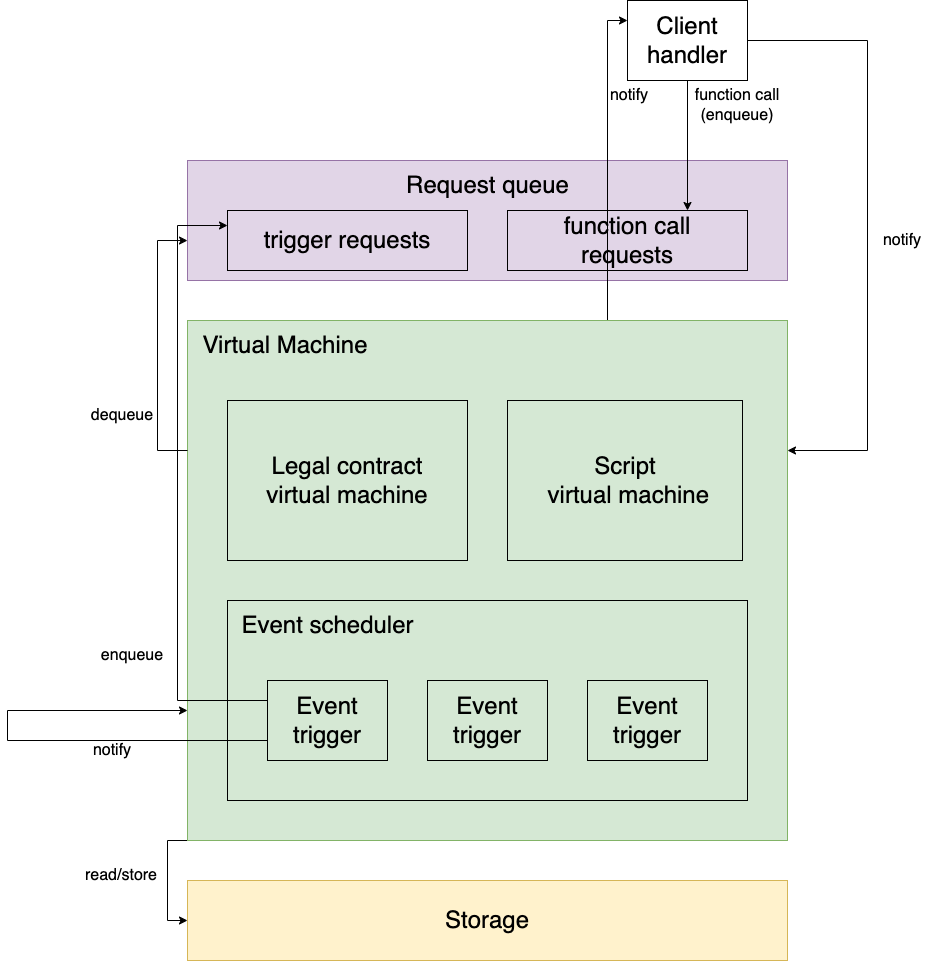
\includegraphics[width=0.9\textwidth]{immagini/capitolo-5/vm.png}
		\caption{Virtual machine.}
		\label{fig:vm}
	\end{center}
\end{figure}

\subsection{Requests queue}

This component implements a \textit{queue} that collects all requests made by clients and events for the 
execution of obligations. In the \textit{Stipula} language, for a contract, if at the same time $t$ a 
request from the client to perform a function and a request to perform an obligation arrive 
simultaneously, the execution of the obligation takes \textbf{precedence} over the execution of the 
function requested by the client. To do this, the \verb|RequestQueue| manages two queues: one queue 
collects client requests (\verb|functionCallRequests|) and one queue collects obligation execution 
requests (\verb|obligationRequests|). The \verb|RequestQueue| object has two main methods:
\begin{enumerate}
   \item \verb|enqueue|: this method allows you to add a request to the queue;
   \item \verb|dequeue|: this method allows you to get a request from one of the two queues. If the 
   \verb|obligationRequests| has items, this method will return an item from this queue. If the 
   \verb|obligationRequests| is empty, then an item from the \verb|functionCallRequests| queue will be 
   returned.
\end{enumerate}

Access to these queues is controlled by a \textit{mutex}, in order to properly handle precedence between 
requests. The approach used in the current implementation of the architecture may be a performance 
limitation. In the next chapter some optimizations have been proposed (see \ref{optimizations}).

\subsection{Legal Contract Virtual Machine}
\label{legal-contract-vm}

This component performs contract functions written in \textit{Stipula bytecode}. The instructions of 
this virtual machine are those listed in the \ref{table:bytecode-instructions} table. The functioning of 
this component is very simple: given as input a function of a contract written in bytecode and the 
arguments of this function, the virtual machine sequentially executes each instruction. If one or more 
errors are thrown during the execution of the function, the virtual machine interrupts the execution and 
returns the errors in a special \textit{error stack}; otherwise, execution proceeds until the \verb|HALT| 
instruction is reached, which corresponds to the end of the function.

In this virtual machine there are several \textit{memory zones}:
\begin{enumerate}
  \item \verb|stack|: this is the memory area used by the virtual machine to manipulate the values by 
  means of the instructions read;
  \item \verb|scopeSpace|: this space is dedicated to the storage of local variables to the function;
  \item \verb|argumentsSpace|: this space is dedicated to storing the arguments of the function;
  \item \verb|globalSpace|: this space is dedicated to storing global variables of the contract instance. 
  This space is valued through the information saved in the \textit{Storage} module;
  \item \verb|singleUseSealsToCreate|: this space is dedicated to the temporary storage of the 
  \textit{single-use-seals} to be created. When a function whose code expects to perform one or more 
  \textit{Pay-to-Party} is executed, the execution is not momentarily interrupted to send the payments. We 
  want to ensure atomicity in the execution of the code of a function. Therefore, when the virtual machine 
  realizes that it needs to make a payment to one or more users, it temporarily stores the 
  single-use-seals it has to create. Once the virtual machine finishes executing the function and the 
  execution has not generated any errors, then we will proceed to perform the different 
  \textit{Pay-to-Party};
  \item \verb|createEventRequests|: similarly to the previous point, when the virtual machine reads the 
  \verb|TRIGGER <obligation_function_name>| instruction, it stores in this dedicated space all the events 
  it will have to create once the execution of the function has finished.
\end{enumerate}

In addition, there are two other important fields:
\begin{enumerate}
  \item \verb|executionPointer|: this field indicates the current instruction that has been executed;
  \item \verb|offset|: a full contract is never input to the virtual machine. Only the code of the 
  function to be executed is loaded, therefore the initial value of the \verb|executionPointer| will 
  always be zero. However, when debugging a contract it is useful to have a reference to the line of 
  code that threw an error against the full code of the contract, and not the local code of the function. 
  For this reason, this field stores the line number where the function code starts in the contract and 
  when an error is thrown, in the logs it is possible to have both the line number local to the function 
  and the global line number of the complete contract . Thus, the line number that takes into account the 
  position it is in the contract is given by $\verb|offset| + \verb|executionPointer|$.
\end{enumerate}

\subsection{Script Virtual Machine}
\label{script-vm}

\subsubsection{Single-use-seal and Ownership}
\label{single-use-seals-and-ownerships}

In the previous chapter, the concept of \textit{single-use-seal} (see \ref{single-use-seal-definition}) 
was introduced as a model for asset management. The structure of a single-use-seal was introduced earlier 
(see \ref{pay-to-contract}). To ensure that a single-use-seal can only be spent by the rightful owner, 
this seal is \textit{blocked} using a specific program written in \textit{Script} language. This program 
is saved in the \verb|lockScript| field and is stored along with the other single-use-seal information. 
If a user wants to spend a specific single-use-seal, he must provide proof to prove rightful ownership of 
the funds. The proof is coded as another program written in \textit{Script}, which allows you to 
\textit{unlock} the \verb|unlockScript| program. When a user provides this program as proof of ownership 
of the single-use-seal, he is demonstrating the \textit{ownership} of the funds. In fact, when a user 
wants to make a \textit{Pay-to-Contract}, the user provides the proof in the \verb|FunctionCall| message 
(see section \ref{ownership}). The proof is coded in the Java object \verb|Ownership| and is structured 
as follows:
\begin{enumerate}
  \item \verb|String contractInstanceId|: it indicates to which instance of the contract the payment must 
  be made;
  \item \verb|SingleUseSeal singleUseSeal|: indicate the funds to be spent;
  \item \verb|String unlockScript|: the program that allows you to unlock the \verb|lockScript| contained 
  in the \verb|singleUseSeal| object.
\end{enumerate}

Joining \verb|unlockScript| and \verb|lockScript| it is possible to check if the user is the actual owner 
of the single-use-seal he wants to spend. The main idea of this mechanism was formulated in Bitcoin in 
2009 and is called \textbf{Pay-to-Public-Key-Hash} (\textbf{P2PKH}) \autocite{book:mastering-bitcoin}. 
This was one of the very first mechanisms to be able to make payments in the Bitcoin network. The 
\verb|lockScript| program can only be unlocked if in the \verb|unlockScript| program cryptographic proof 
is provided via the funds holder's private key. In this way, when a user wants to pay for an instance of 
a contract, it is the user himself who voluntarily transfers the \textit{ownership} of a single-use-seal 
to the instance of the contract.

\subsubsection{Script}

In the previous chapter, the \textit{Script} language was introduced (see \ref{script-language}). The 
instructions of this language are very limited and most of them are separate from the instructions of the 
\textit{Legal Contract Virtual Machine}. The instructions of the \textit{Script Virtual Machine} are 
listed in the \ref{table:instructions-svm} table and it is possible to notice the difference in the sets 
of instructions between the two virtual machines in the image \ref{fig:instructions-vms} . Furthermore, 
this language only allows you to handle values that are of type \verb|bool| or \verb|str| (see image 
\ref{fig:types-vms}).

\begin{ThreePartTable}
	\setTableNoteFont{\footnotesize}
  \begin{longtable}{|c|c|}
    \caption{Table of \textit{Script Virtual Machine} instructions.}
    \label{table:instructions-svm}\\
    \noalign{\global\arrayrulewidth0.7pt}
    \hline
    \textbf{Instruction} & \textbf{Behavior} \\ [5pt]
    
    \noalign{\global\arrayrulewidth0.7pt}
    \hline
    
    \verb|PUSH|     & $- \rightarrow *$ \\
    \hline
    
    \verb|HALT|     & $- \rightarrow -$ \\
    \hline
    
    \verb|DUP|      & $* \rightarrow (*, *)$ \\
    \hline

    \verb|SHA256|   & $\verb|str| \rightarrow \verb|str|$ \\
    \hline

    \verb|EQUAL|    & $(\verb|str|, \verb|str|) \rightarrow - || \verb|str|$ \\
    \hline
    
    \verb|CHECKSIG| & $(\verb|str|, \verb|str|) \rightarrow \verb|bool|$ \\
    
    \noalign{\global\arrayrulewidth0.7pt}
    \hline
  \end{longtable}
\end{ThreePartTable}

\begin{figure}[htbp]
	\begin{center}
		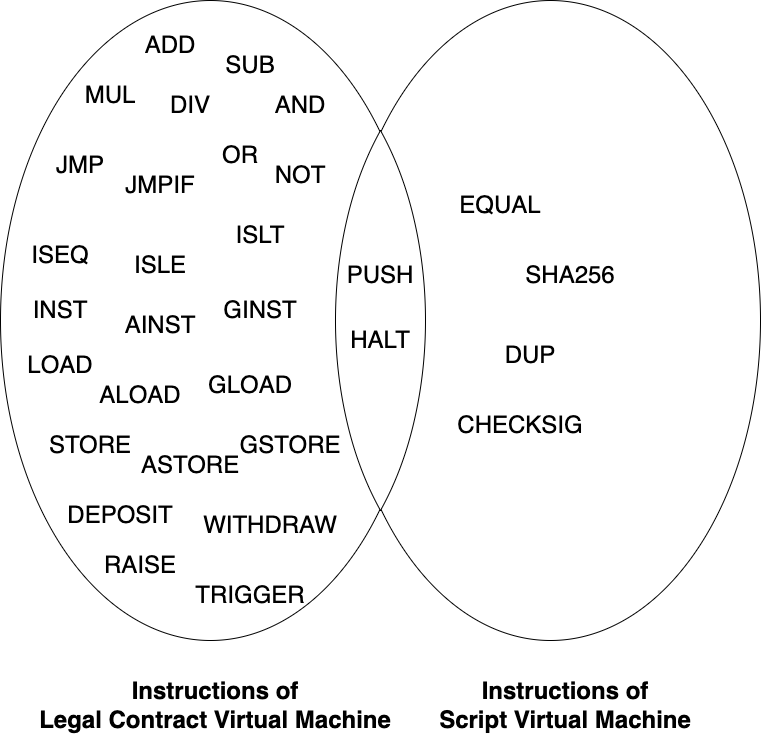
\includegraphics[height=8cm]{immagini/capitolo-5/instructions-vms.png}
		\caption{The instruction sets of the two virtual machines.}
		\label{fig:instructions-vms}
	\end{center}
\end{figure}

\begin{figure}[htbp]
	\begin{center}
		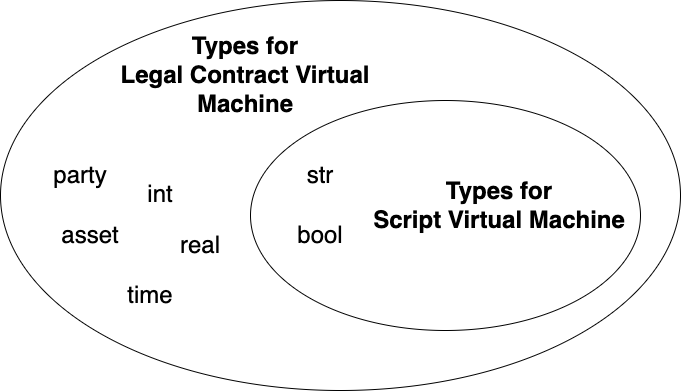
\includegraphics[width=0.8\textwidth]{immagini/capitolo-5/types-vms.png}
		\caption{Sets of the types of the two virtual machines.}
		\label{fig:types-vms}
	\end{center}
\end{figure}

\paragraph{PUSH and HALT}

These statements have the same behavior as those defined for the \textit{Legal Contract Virtual Machine}. 
The only difference is that these statements operate only on values of type \verb|bool| and \verb|str|.

\paragraph{DUP}

This statement takes a value of any type as input and outputs two values that have the same type as the 
input value. This \textit{duplicates} the value received as input, that is, it \textit{pops} from the 
stack and performs two \textit{pushes} of the same value.

\paragraph{SHA256}

This instruction takes as input a value of type \verb|str| and outputs a value of the same type. This 
instruction calculates the SHA256 hash of the input value.

\paragraph{EQUAL}

Given two inputs of type \verb|str|, this statement checks whether the two strings are \textit{equal}. If 
the two values are equal, no value is returned, if instead the values are not equal, then a value of type 
\verb|str| in the \textit{error stack} of the virtual machine.

\paragraph{CHECKSIG}

This instruction takes as input two values of type \verb|str| and outputs a value of type \verb|bool|. The 
first value represents a \textit{public key}, while the second represents a \textit{signature}. This 
instruction allows you to check if, using the public key received as input, the signature is valid or not.

\paragraph{Instruction table}

A summary table of the instructions is shown below: the \verb|-| symbol means that the statement takes no 
value as input or returns no value as output, while the \verb|*| means that the instruction accepts a 
value or outputs a value of type \verb|bool| or \verb|str|.

\subsubsection{LockScript and UnlockScript}
\label{lock-script-and-unlock-script}

Having illustrated the \textit{Script} and \textit{P2PKH} language, give the well-defined structure of 
\verb|lockScript| and \verb|unlockScript|: % citare https://github.com/federicozanardo/stipula-node/issues/23
\begin{enumerate}
  \item \verb|lockScript|: \verb|DUP SHA256 PUSH str <pub_key_hash> EQUAL CHECKSIG|;
  \item \verb|unlockScript|: \verb|PUSH str <signature> PUSH str <pub_key>|;
\end{enumerate}

where,
\begin{enumerate}
  \item \verb|<pub_key>|: is the public key of the user in possession of the single-use-seal;
  \item \verb|<pub_key_hash>|: corresponds to the SHA256 hash of the public key;
  \item \verb|<signature>|: corresponds to the signature of the identifier of the single-use-seal to be 
  spent.
\end{enumerate}

The \verb|<signature>| corresponds to the cryptographic proof that only the user can provide to 
demonstrate possession of the single-use-seal. Signing the single-use-seal identifier provides 
\textit{unique} cryptographic proof and cannot be reused to prove ownership of other funds. So, when the 
user sends the signature and his public key to a \textit{Stipula} server or node, anyone can check it. 
Therefore, if the signature were made using information that can be \textit{reused} to prove possession of 
multiple funds, this would lead to a major security problem, as anyone can verify the signature and reuse 
the information used in the signature to misappropriate other funds.

The union of \verb|lockScript| and \verb|unlockScript|, create the following program which will be 
validated by the virtual machine:

\begin{Verbatim}[numbers=left,xleftmargin=1cm,firstnumber=1,breaklines=true,breakanywhere=true,tabsize=2]
  PUSH str <signature> PUSH str <pub_key> DUP SHA256 PUSH str <pub_key_hash> EQUAL CHECKSIG
\end{Verbatim}

\newpage
The program is evaluated as follows (an example is illustrated by observing the evolution of the stack):
\begin{enumerate}
  \item \verb|PUSH str <signature>|: la \verb|<signature>| is loaded onto the stack
  \begin{ThreePartTable}
    \setTableNoteFont{\footnotesize}
    \begin{longtable}{|>{\centering\arraybackslash}p{2.5cm}|}
      %\label{table:instructions-svm}\\
      \noalign{\global\arrayrulewidth0.7pt}
      \hline

      \\
      \hline
      
      \\
      \hline
      
     \\
      \hline
  
      \\
      \hline
  
      \\
      \hline
      
      \verb|<signature>| \\
      
      \noalign{\global\arrayrulewidth0.7pt}
      \hline
    \end{longtable}
  \end{ThreePartTable}

  \item \verb|PUSH str <pub_key>|: the public key is loaded onto the stack
  \begin{ThreePartTable}
    \setTableNoteFont{\footnotesize}
    \begin{longtable}{|>{\centering\arraybackslash}p{2.5cm}|}
      %\label{table:instructions-svm}\\
      \noalign{\global\arrayrulewidth0.7pt}
      \hline
      
      \\
      \hline
      
     \\
      \hline
  
      \\
      \hline
  
      \verb|<pub_key>|   \\
      \hline
      
      \verb|<signature>| \\
      
      \noalign{\global\arrayrulewidth0.7pt}
      \hline
    \end{longtable}
  \end{ThreePartTable}

  \item \verb|DUP|: you duplicate the last element of the stack, which in this case is the public key
  \begin{ThreePartTable}
    \setTableNoteFont{\footnotesize}
    \begin{longtable}{|>{\centering\arraybackslash}p{2.5cm}|}
      %\label{table:instructions-svm}\\
      \noalign{\global\arrayrulewidth0.7pt}
      \hline
      
      \\
      \hline
      
     \\
      \hline
  
      \verb|<pub_key>|   \\
      \hline
  
      \verb|<pub_key>|   \\
      \hline
      
      \verb|<signature>| \\
      
      \noalign{\global\arrayrulewidth0.7pt}
      \hline
    \end{longtable}
  \end{ThreePartTable}

  \item \verb|SHA256|: the hash of the last element of the stack is computed, which in this case is the 
  previously duplicated public key
  \begin{ThreePartTable}
    \setTableNoteFont{\footnotesize}
    \begin{longtable}{|>{\centering\arraybackslash}p{2.5cm}|}
      %\label{table:instructions-svm}\\
      \noalign{\global\arrayrulewidth0.7pt}
      \hline
      
      \\
      \hline
  
      \verb|<pub_key_hash>|   \\
      \hline
  
      \verb|<pub_key>|   \\
      \hline
      
      \verb|<signature>| \\
      
      \noalign{\global\arrayrulewidth0.7pt}
      \hline
    \end{longtable}
  \end{ThreePartTable}

  \item \verb|PUSH str <pub_key_hash>|: the public key hash is loaded onto the stack. This hash is taken 
  from the \verb|unlockScript|
  \begin{ThreePartTable}
    \setTableNoteFont{\footnotesize}
    \begin{longtable}{|>{\centering\arraybackslash}p{2.5cm}|}
      \noalign{\global\arrayrulewidth0.7pt}
      \hline
      
      \\
      \hline
      
      \verb|<pub_key_hash>| \\
      \hline
  
      \verb|<pub_key_hash>| \\
      \hline
  
      \verb|<pub_key>|      \\
      \hline
      
      \verb|<signature>|    \\
      
      \noalign{\global\arrayrulewidth0.7pt}
      \hline
    \end{longtable}
  \end{ThreePartTable}

  \newpage
  \item \verb|EQUAL|: occurs if the computed hash is the hash of the \verb|unlockScript| it is equal or 
  less
  \begin{ThreePartTable}
    \setTableNoteFont{\footnotesize}
    \begin{longtable}{|>{\centering\arraybackslash}p{2.5cm}|}
      \noalign{\global\arrayrulewidth0.7pt}
      \hline
      
      \\
      \hline
      
      \\
      \hline
  
      \\
      \hline
  
      \verb|<pub_key>|      \\
      \hline
      
      \verb|<signature>|    \\
      
      \noalign{\global\arrayrulewidth0.7pt}
      \hline
    \end{longtable}
  \end{ThreePartTable}

  \item \verb|CHECKSIG|: occurs if the \verb|<signature>| is valid with the \verb|<pub_key>| present in 
  the stack. If the check is successful, \verb|true| will be pushed onto the stack, otherwise \verb|false|
  \begin{ThreePartTable}
    \setTableNoteFont{\footnotesize}
    \begin{longtable}{|>{\centering\arraybackslash}p{2.5cm}|}
      \noalign{\global\arrayrulewidth0.7pt}
      \hline
      
      \\
      \hline
      
      \\
      \hline
  
      \\
      \hline
  
      \\
      \hline
      
      \verb|true| \\
      
      \noalign{\global\arrayrulewidth0.7pt}
      \hline
    \end{longtable}
  \end{ThreePartTable}
\end{enumerate}

The example just illustrated described all the operations that are performed by the 
\textit{Script Virtual Machine}.

\subsection{Description of the execution flow of a function of a contract}

\begin{figure}[htbp]
	\begin{center}
		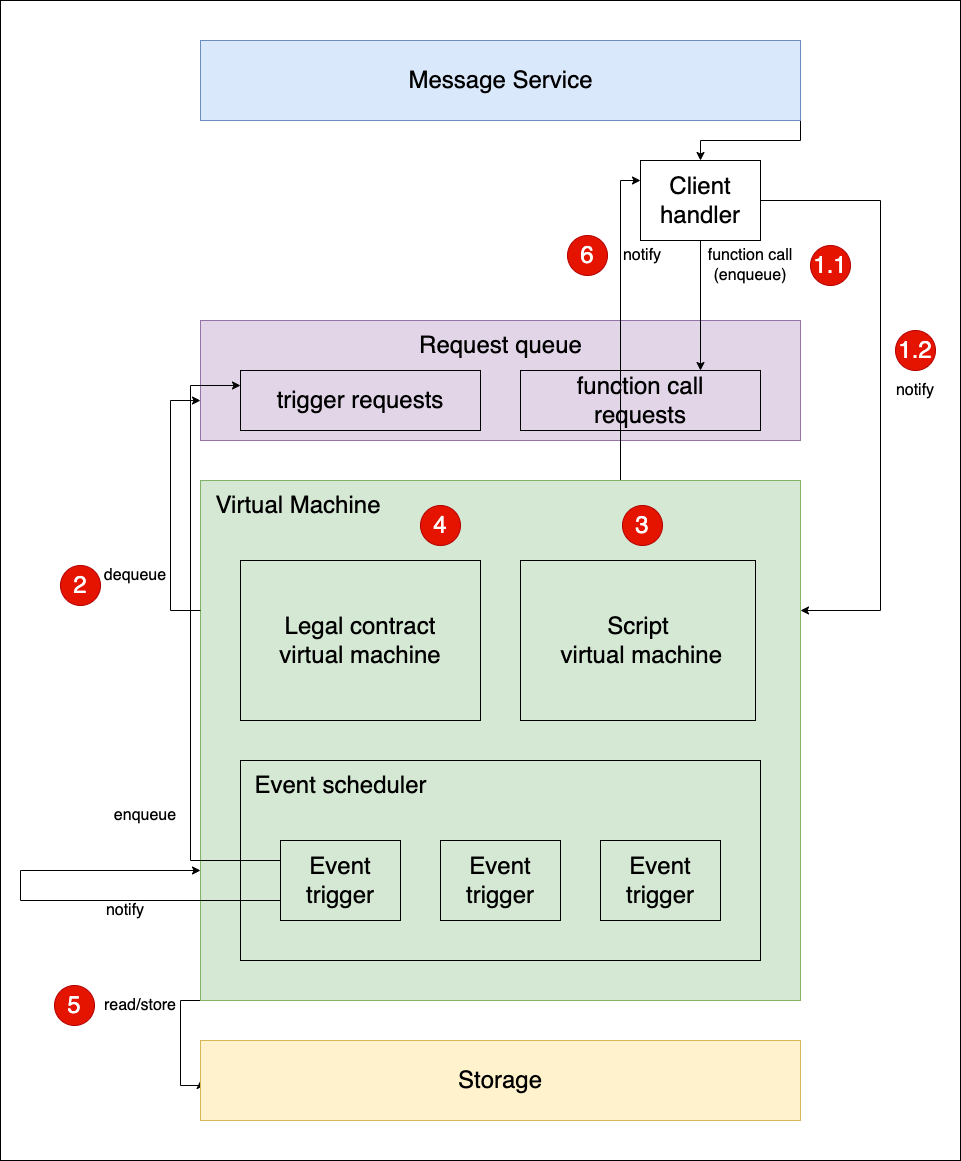
\includegraphics[width=0.9\textwidth]{immagini/capitolo-5/contract-flow.png}
		\caption{Flow of the execution of a function of a function of a contract.}
		\label{fig:contract-flow}
	\end{center}
\end{figure}

This section illustrates the execution flow of a generic contract function (see figure 
\ref{fig:contract-flow}). More precisely, let's suppose that the generic function requires as input a 
value of type \verb|asset|, and that therefore, the user has to make a payment. The flow is as follows:
\begin{enumerate}
  \item A \verb|FunctionCall| message is received (see section \ref{function-call-message}): the 
  \verb|ClientHandler| performs all checks on the format of the message and the signature. After that, the 
  \verb|ClientHandler| adds this new request to the \textit{queue of requests} (\textbf{1.1}, in figure 
  \ref{fig:contract-flow}) and \textit{notifies} the virtual machine (\textbf{1.2}). The notification 
  action of the virtual machine is useful in case the latter is waiting for new requests, but the request 
  queue is empty;
  \item Suppose that the only request in the request queue is the one added in the previous point. The 
  virtual machine dequeues the only request present (\textbf{2});
  \item As mentioned previously, this is a function call that requires an asset as a parameter, therefore, 
  in the \verb|FunctionCall| there is all the information to verify if the funds sent are actually in the 
  user's possession and if they are of the requested quantity. The verification of possession of the sent 
  \textit{single-use-seal} is delegated to the \textit{Script Virtual Machine} (\textbf{3}). If the checks 
  fail, the virtual machine notifies the \verb|ClientHandler| (\textbf{6});
  \item If the verification of the \textit{script} gives a positive result, then we proceed to execute the 
  function indicated by the request. The execution of the function is delegated to the 
  \textit{Legal Contract Virtual Machine} (\textbf{4});
  \item When the execution of the function ends and there are no errors, all the modifications concerning 
  the global variables, the change of the state of the contract and the updating of the single-use-seal, 
  which now can no longer be spent in other contract instances are sent to the \textit{Storage} module 
  (\textbf{5});
  \item Finally, the virtual machine notifies the \verb|ClientHandler|, returning a response regarding the 
  success or failure of the function execution (\textbf{6}).
\end{enumerate}

Next, concrete examples of some contract examples will be shown (see section \ref{examples}). 

\subsection{Pay-to-Party}

Previously, we discussed \textit{Pay-to-Contract}, that is, how a user makes a payment to an instance of 
a contract. When, on the other hand, it is the instance of a contract that has to send payments to one or 
more users, this method is called \textit{Pay-to-Party}. Again, this concept was introduced in the 
previous chapter (see \ref{pay-to-contract-and-pay-to-party}). This mechanism is much simpler than 
\textit{Pay-to-Contract}. When a certain function of a contract expects to send a payment to a user, the 
virtual machine performs all the preliminary checks, for example, it makes sure that it does not disappear 
by the amount of assets from the funds present in the contract instance. Once these checks have been made, 
the virtual machine creates new \textit{single-use-seals}, locking them with the public key of the 
recipient of the funds. Specifically, the \verb|lockScript| will have the following structure: 
\verb|DUP SHA256 PUSH str <pub_key_hash> EQUAL CHECKSIG|, where \verb|<pub_key_hash>| corresponds to the 
SHA256 hash of the payment recipient's public key; By doing so, these funds are now no longer owned by 
the contract instance, but by a specific user. As explained above (see 
\ref{lock-script-and-unlock-script}), only the new owner of the funds will be able to spend them.

\subsection{Obligations}

In the context of the \textit{Stipula} language, \textit{obligations} are formulated into commitments that 
are verified at a given time and issue a corresponding penalty if the obligation has not been fulfilled. 
From an implementation point of view, an obligation consists in the \textit{scheduling} of a 
\textit{event} which at a given moment will call a specific function of the contract. If the obligation 
has been fulfilled, then there won't be the conditions to be able to execute the function, otherwise the 
virtual machine will execute the function, applying penalties.

\subsubsection{Scheduling of an event and description of the flow of execution of an obligation}
\label{execution-flow-for-obligation}

Scheduling always occurs through the execution, by a function, of a piece of code similar to the 
following:

\begin{Verbatim}[numbers=left,xleftmargin=1cm,firstnumber=1,tabsize=2]
  ...
  GLOAD waitTime
  PUSH time now
  ADD
  TRIGGER obligation_1
  ...
\end{Verbatim}

where, from line 2 to line 4 we define the time $t$ in which the obligation must be performed (if the 
conditions allow it), and in line 5 we specify which function must be performed at time $t $. When the 
machine finishes executing the function, a \verb|CreateEventRequest| object is created, in which the name 
of the function to be called and the time $t$ in which this function must be called must be present. After 
that, this object is incorporated into the \verb|EventSchedulingRequest| object, which also contains 
information about the contract instance. This last object is added to a list of \verb|EventTrigger|, 
managed by \verb|EventScheduler|, which collects all the scheduled events. \verb|EventTrigger| is an 
object that extends the \verb|TimerTask| class, which allows you to create a thread and carry out tasks 
at a set time $t$. From here we illustrate the execution flow (see figure \ref{fig:obligation-flow}):
\begin{enumerate}
  \item When the time $t$ is reached, the \verb|EventTrigger| adds the \verb|EventSchedulingRequest| 
  object to the request queue (\textbf{1.1}). This way, the next request that the virtual machine 
  executes will be a request to perform an obligation. After that, \verb|EventTrigger| notifies the 
  virtual machine if it is waiting for new requests, but the request queue is empty (\textbf{1.2});
  \item Suppose that the only request in the request queue is the one added in the previous point. The 
  virtual machine dequeues the only request present (\textbf{2});
  \item If the conditions are satisfied, the virtual machine proceeds to execute the function that 
  represents the obligation, and therefore, to apply the penalties; otherwise the virtual machine does 
  not perform the function. The condition for being able to perform an obligation is if the current state 
  of the contract instance coincides with the state in which the obligation must be performed (\textbf{3});
  \item When the execution of the function ends and there are no errors, all the modifications concerning 
  the global variables, the change of the state of the contract and the updating of the single-use-seal, 
  which now can no longer be spent in other contract instances are sent to the \textit{Storage} module 
  (\textbf{4});
\end{enumerate}

Next, concrete examples of some contract examples will be shown (see section \ref{examples}).

\begin{figure}[htbp]
	\begin{center}
		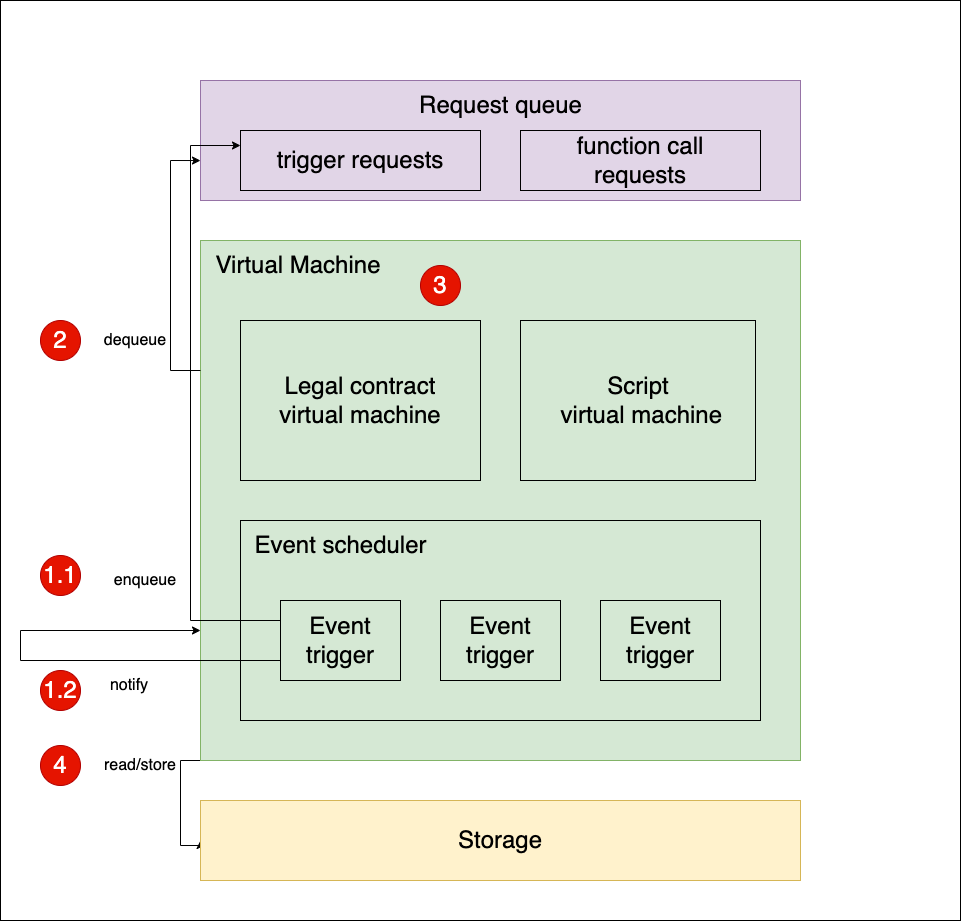
\includegraphics[width=0.9\textwidth]{immagini/capitolo-5/obligation-flow.png}
		\caption{Flow of execution of an obligation.}
		\label{fig:obligation-flow}
	\end{center}
\end{figure}

\section{Storage}
\label{storage}

This module allows you to store all the information regarding contracts, contract instances and their 
evolution, assets and all asset transfers between users and contract instances.

\subsection{LevelDB}

\textit{LevelDB} \autocite{site:leveldb} is an open source \textit{key-value storage library} developed by 
Google. It is a light, fast and efficient storage system capable of handling large amounts of data. 
LevelDB is designed to provide an ordered key-value store with high performance for read and write 
operations. Keys and values can be of any length, and the data is sorted by key in a natural order. The 
data is stored as a \textit{binary blob} and the key can be any stream of bytes. However, it is important 
to note that LevelDB is an unstructured database, which means it doesn't enforce a particular schema or 
data model, and it is up to the application developer to define how to organize and access the data. For 
simplicity in the development of the architecture, it was decided to archive the Java objects directly, 
without designing a particular structure, if not following the key-value structure offered by the library.

LevelDB supports various operations, including basic \textit{CRUD} operations (\textit{create}, 
\textit{read}, \textit{update}, \textit{delete}), \textit{batch} operations, and \ textit{snapshot}.

LevelDB is a library written in C++, but it also has \textit{bindings} for other languages, such as Java, 
Python and Go. This library is used in various applications, including the Bitcoin and Ethereum 
blockchains.

\subsection{Structure}

The \textit{Storage} module consists mainly of four components (see figure \ref{fig:storage-structure}):
\begin{enumerate}
  \item \textit{Asset storage}: all the data concerning the definition of the assets are stored in this 
  component;
  \item \textit{Ownerships storage}: this component stores all spent and unspent \textit{single-use-seals};
  \item \textit{Contracts storage}: this component has the task of storing all the information concerning 
  the contract, such as the source code, the bytecode and the information for instantiating a state 
  machine;
  \item \textit{Contract instances storage}: this component stores all the information that allows you to 
  track the evolution of the state of a contract instance.
\end{enumerate}

\begin{figure}[htbp]
	\begin{center}
		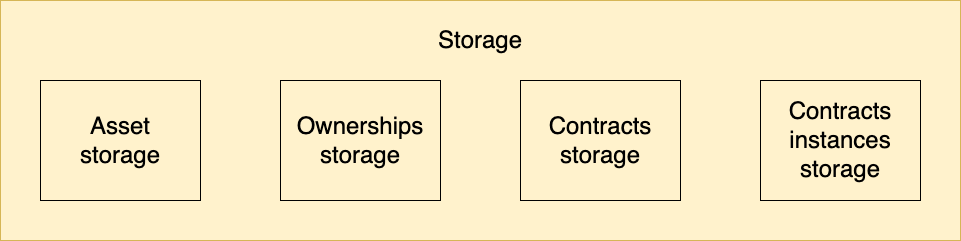
\includegraphics[width=0.9\textwidth]{immagini/capitolo-5/storage.png}
		\caption{Structure of the \textit{Storage} module.}
		\label{fig:storage-structure}
	\end{center}
\end{figure}

\paragraph{Storage serializer}

There are two operations that unite all the components that allow information to be stored and they are:
\begin{enumerate}
  \item \verb|byte[] serialize(T data)|: this method allows you to serialize the data received as input, 
  that is, transforming the input data into a stream of output bytes;
  \item \verb|T deserialize(byte[] bytes)|: this method allows you to deserialize the byte stream 
  received as input into a target object \verb|T|.
\end{enumerate}

Each component of this module extends this class.

\paragraph{Asset storage}

In this class there is a main method, \verb|getAsset|, which allows to obtain all the information 
concerning a specific asset, given an asset identifier as input. There is another method, \verb|seed|, 
which allows you to initialize a certain number of assets when starting the \textit{Stipula} instance. 
This is a method that will be removed in the future: the need for this method to exist is closely related 
to the current limitations of the architecture. See section \ref{database-seeding}, to see how database 
\textit{seeding} can be done, and section \ref{creation-assets-and-distribution} to see a possible 
solution to this limitation.

\paragraph{Ownerships storage}

Also in this class there is the \verb|seed| method, which allows you to create, in a hard-coded way, 
\textit{single-use-seals} for some users. The reason is the same as the one expressed previously, that is, 
the need for this method is due to the current limitations of the implemented architecture.

The other methods in this class are:
\begin{enumerate}
  \item \verb|getFunds|: this method allows you to get all the funds, given a specific input address;
  \item \verb|getFund|: this method allows you to obtain the information of a specific \textit{ownership}, 
  given the property identifier and an address;
  \item \verb|addFunds|: with this method it is possible to add \textit{ownership} to different addresses;
  \item \verb|makeOwnershipSpent|: this method allows you to update a specific \textit{ownership} as 
  \textit{spent}. This method requires as input:
  \begin{enumerate}
    \item The \textit{address} to which the \textit{ownership} is associated;
    \item The identifier of the \textit{ownership} to update;
    \item The identifier of the instance of the contract: this information is important as it is useful to 
    trace from which instance of the contract the payment was made;
    \item \verb|unlockScript|: once the virtual machine has validated the \textit{script} which allows to 
    certify the user's possession of the \textit{ownership}, the missing part of the script is saved, 
    i.e. \verb|unlockScript|. By doing so, this \textit{ownership} can now no longer be spent.
  \end{enumerate}
\end{enumerate}

\paragraph{Contracts storage}

This class contains the following methods:
\begin{enumerate}
  \item \verb|getContract|: this method allows you to obtain information about a specific contract, given 
  the identifier of an input contract;
  \item \verb|saveContract|: this method allows you to store a new contract. If this method is called, 
  the contract has been compiled successfully.
\end{enumerate}

Once a contract is stored in this form, it can no longer be deleted or modified.

\paragraph{Contract instances storage}

This class contains the following methods:
\begin{enumerate}
  \item \verb|getContractInstance|: this method allows to obtain the information of a specific instance of 
  a contract, given the identifier of an instance of an input contract;
  \item \verb|saveContractInstance|: this method allows you to create a new instance of a contract. If 
  this method is called, it means that the \textit{agreement} phase has been successful;
  \item \verb|storeGlobalSpace|: this method allows you to update the \textit{global variables} of a 
  specific instance of a contract. If this method is called, it means that the function execution was 
  successful;
  \item \verb|storeStateMachine|: this method allows you to update the \textit{current state} of the state 
  machine of a contract instance. If this method is called, it means that the function execution was 
  successful.
\end{enumerate}

\section{Examples}
\label{examples}

In this section, concrete examples of code will be introduced to illustrate how the implemented 
implementation works. Examples will include writing the contract in \textit{Stipula}, loading and 
compiling the contract, and running an instance of the contract.

\subsection{Asset swap}
\label{asset-swap}

In this example, there are two actors, Alice and Bob, who want to trade two assets. For simplicity, the 
price variation that these assets may have over time is not taken into consideration, the exchange rate of 
these two assets is fixed by the parties to the contract when a new instance of the contract is made.

For this example there are two versions: in the first version, when Bob deposits his asset, the swap 
happens immediately; in the second version, when both parties deposit their assets, the swap is delegated 
to a \textit{obligation}, which will be triggered after a certain time indicated by the variable 
\verb|waitTimeBeforeSwapping|.

The complete code is present in the appendix \ref{app:asset-swap-complete-code}.

\subsubsection{Agreement}

This first part of the contract defines the variables for:
\begin{enumerate}
  \item The assets: the identifiers of the assets to be exchanged in this contract are specified (line 2);
  \item The quantities of assets to be traded (line 3);
  \item The initial state of the contract state machine (line 4).
\end{enumerate}

\begin{Verbatim}[numbers=left,xleftmargin=1cm,firstnumber=1,breaklines=true,tabsize=2]
  stipula SwapAsset {
    asset assetA:stipula_assetA_ed8i9wk, assetB:stipula_assetB_pl1n5cc
    field amountAssetA, amountAssetB
    init Inactive
\end{Verbatim}

When two parties decide to exchange two specific assets, they make a \textit{agreement}. In the code of 
this function it is possible to notice that the participants of the contract are defined and the values 
for \verb|amountAssetA| and \verb|amountAssetB|, that is, indicate the amount of assets that will have to 
be exchanged. Once this function has been called it means that both parties to the contract are in 
agreement to trade those particular assets, at an agreed rate.

\begin{Verbatim}[numbers=left,xleftmargin=1cm,firstnumber=6,tabsize=2]
  agreement (Alice, Bob)(amountAssetA, amountAssetB) {
        Alice, Bob: amountAssetA, amountAssetB
    } ==> @Inactive
\end{Verbatim}

\newpage
The following bytecode is associated with this function in \textit{Stipula}:
\begin{Verbatim}[numbers=left,xleftmargin=1cm,firstnumber=1,tabsize=2]
  fn agreement Alice,Bob Inactive real,real
  global:
  GINST party Alice
  GINST party Bob
  GINST asset assetA 2 stipula_assetA_ed8i9wk
  GINST asset assetB 2 stipula_assetB_pl1n5cc
  GINST real amountAssetA 2
  GINST real amountAssetB 2
  args:
  PUSH party :Alice
  GSTORE Alice
  PUSH party :Bob
  GSTORE Bob
  PUSH real :amountAssetA
  GSTORE amountAssetA
  PUSH real :amountAssetB
  GSTORE amountAssetB
  start:
  end:
  HALT
\end{Verbatim}

In line 1 it is possible to note the signature of the function, where the name of the function 
(\verb|agreement|), the participants of the contract (\verb|Alice,Bob|), the state in which the instance 
of the contract will go once the execution of the function will have terminated without errors 
(\verb|Inactive|) and the types of the parameters of the function (\verb|real,real|). In this case, the 
function takes two parameters and both must be of type \verb|real|.

From line 2 to line 8, the global variables of the contract are created, i.e. the participants of the 
contract (lines 3-4), the variables that will contain the assets that will have to be exchanged 
(lines 5-6) and the variables that indicate the amount of assets that will have to be deposited 
(lines 7-8).

From line 9 to line 17, the global variables are valued using the values contained in the function 
parameters. In particular:
\begin{enumerate}
  \item Lines 10-13: information about the parties to the contracts is stored (public key and address);
  \item Lines 14-17: the variables indicating the quantity of assets that must be deposited in the 
  contract by each participant in the contract are set.
\end{enumerate}

From line 18 to line 19 the body of the function is defined, which in this case is empty, and in line 20 
the end of the function is indicated by the function \verb|HALT|.

\subsubsection{Deposit of the first asset}

This portion of code allows Alice to deposit a certain amount of assets, agreed during the 
\textit{agreement} phase. In particular:
\begin{enumerate}
  \item Line 10: this function can only be called by Alice and if the contract is in the \verb|@Inactive| 
  state. Note that this function takes a \verb|asset| as an argument (note \verb|[y]|);
  \item Line 11: a check is made to verify if the quantity received as input is equal to the quantity 
  established in the \textit{agreement} phase;
  \item Line 12: this instruction represents the deposit of a certain quantity of assets within the 
  instance of the contract;
  \item Line 14: at the end of the function, the state of the contract will change from \verb|@Inactive| 
  to \verb|@Swap|.
\end{enumerate}

\begin{Verbatim}[numbers=left,xleftmargin=1cm,firstnumber=10,tabsize=2]
  @Inactive Alice : depositAssetA()[y]
        (y == amountAssetA) {
            y -o assetA;
            _
    } ==> @Swap
\end{Verbatim}

The following bytecode is associated with this function in \textit{Stipula}:
\begin{Verbatim}[numbers=left,xleftmargin=1cm,firstnumber=21,tabsize=2]
  fn Inactive Alice depositAssetA Swap asset
  args:
  PUSH asset :y
  AINST asset :y
  ASTORE y
  start:
  ALOAD y
  GLOAD amountAssetA
  ISEQ
  JMPIF if_branch
  RAISE AMOUNT_NOT_EQUAL
  JMP end
  if_branch:
  ALOAD y
  GLOAD assetA
  DEPOSIT assetA
  end:
  HALT
\end{Verbatim}

On line 21 it is possible to note the signature of the function, where the following are specified:
\begin{enumerate}
  \item The state the contract instance must be in in order to call this function (\verb|@Inactive|);
  \item The party that can call this function (\verb|Alice|);
  \item The name of the function (\verb|depositAssetA|);
  \item The state the contract instance will go to once the function's execution has finished without 
  errors (\verb|Swap|);
  \item The type of the function parameter (\verb|asset|).
\end{enumerate}

From line 22 to line 25, the function argument is instantiated. This variable is stored in the argument 
space (\verb|argumentSpace|).

From line 26 to line 37 is the body of the function. In particular, from line 27 to line 30, the virtual 
machine checks if the quantity of assets received as input is equal to that established during the 
\textit{agreement} phase. If the result of this check is \textit{false}, then the virtual machine will 
continue executing first with line 31 and then with line 32, the function execution will terminate. If 
instead the result of the check is \textit{true}, starting from line 30, the virtual machine will execute 
the instructions starting from line 33 in sequence.

From line 34 to line 36, it is possible to note the effective action of \textit{deposit} of assets within 
the instance of the contract (\textit{Pay-to-Contract}). In particular:
\begin{Verbatim}[numbers=left,xleftmargin=1cm,firstnumber=33,tabsize=2]
  ...
  ALOAD y
  GLOAD assetA
  DEPOSIT assetA
  ...
\end{Verbatim}
corresponds to the following line written in \textit{Stipula}
\begin{Verbatim}[numbers=left,xleftmargin=1cm,firstnumber=11,tabsize=2]
  ...
          y -o assetA;
  ...
\end{Verbatim}

\subsubsection{Deposit of the second asset and swap}

The code of this function is very similar to that of the previous function, except for the \textit{swap} 
operation. This function, in fact, allows Bob to deposit the asset in his possession and then to exchange 
the assets between the participants of the contract. In particular, it is possible to observe that line 19 
and line 20 implement the actual asset swap operation, ie: the asset previously deposited by Alice is sent 
to Bob; the asset deposited in this function by Bob is sent to Alice.

\begin{Verbatim}[numbers=left,xleftmargin=1cm,firstnumber=16,tabsize=2]
  @Swap Bob : depositAssetBAndSwap()[y]
        (y == amountAssetB) {
            y -o assetB
            assetB -o Alice
            assetA -o Bob;
            _
    } ==> @End
  }
\end{Verbatim}

The following bytecode is associated with this function in \textit{Stipula}:
\begin{Verbatim}[numbers=left,xleftmargin=1cm,firstnumber=39,tabsize=2]
  fn Swap Bob depositAssetBAndSwap End asset
  args:
  PUSH asset :y
  AINST asset :y
  ASTORE y
  start:
  ALOAD y
  GLOAD amountAssetB
  ISEQ
  JMPIF if_branch
  RAISE AMOUNT_NOT_EQUAL
  JMP end
  if_branch:
  ALOAD y
  GLOAD assetB
  DEPOSIT assetB
  PUSH real 100 2
  GLOAD assetB
  GLOAD Alice
  WITHDRAW assetB
  PUSH real 100 2
  GLOAD assetA
  GLOAD Bob
  WITHDRAW assetA
  end:
  HALT
\end{Verbatim}

Again, the bytecode produced is very similar to that produced for the previous function. It can be seen 
that from line 55 to line 62 the asset swap is implemented. In particular, it is possible to note:
\begin{enumerate}
  \item From line 52 to line 54 there is a \textit{deposit} (\textit{Pay-to-Contract})
  \begin{Verbatim}[numbers=left,xleftmargin=1cm,firstnumber=51,tabsize=2]
    ...
    ALOAD y
    GLOAD assetB
    DEPOSIT assetB
    ...
  \end{Verbatim}
  This piece of code corresponds to the following line written in \textit{Stipula}
  \begin{Verbatim}[numbers=left,xleftmargin=1cm,firstnumber=17,tabsize=2]
    ...
            y -o assetB;
    ...
  \end{Verbatim}
  \item From line 55 to line 58 there is a \textit{withdraw} towards Alice (\textit{Pay-to-Party})
  \begin{Verbatim}[numbers=left,xleftmargin=1cm,firstnumber=54,tabsize=2]
    ...
    PUSH real 100 2
    GLOAD assetB
    GLOAD Alice
    WITHDRAW assetB
    ...
  \end{Verbatim}
  This piece of code corresponds to the following line written in \textit{Stipula}
  \begin{Verbatim}[numbers=left,xleftmargin=1cm,firstnumber=18,tabsize=2]
    ...
            assetB -o Alice;
    ...
  \end{Verbatim}
  \item From line 59 to line 62 there is a \textit{withdraw} towards Bob (\textit{Pay-to-Party})
  \begin{Verbatim}[numbers=left,xleftmargin=1cm,firstnumber=58,tabsize=2]
    ...
    PUSH real 100 2
    GLOAD assetA
    GLOAD Bob
    WITHDRAW assetA
    ...
  \end{Verbatim}
  This piece of code corresponds to the following line written in \textit{Stipula}
  \begin{Verbatim}[numbers=left,xleftmargin=1cm,firstnumber=19,tabsize=2]
    ...
            assetA -o Bob;
    ...
  \end{Verbatim}
\end{enumerate}

\subsubsection{Example of execution}

An example of execution of this contract is illustrated.

\paragraph{Deploy contract}

\begin{figure}[htbp]
	\begin{center}
		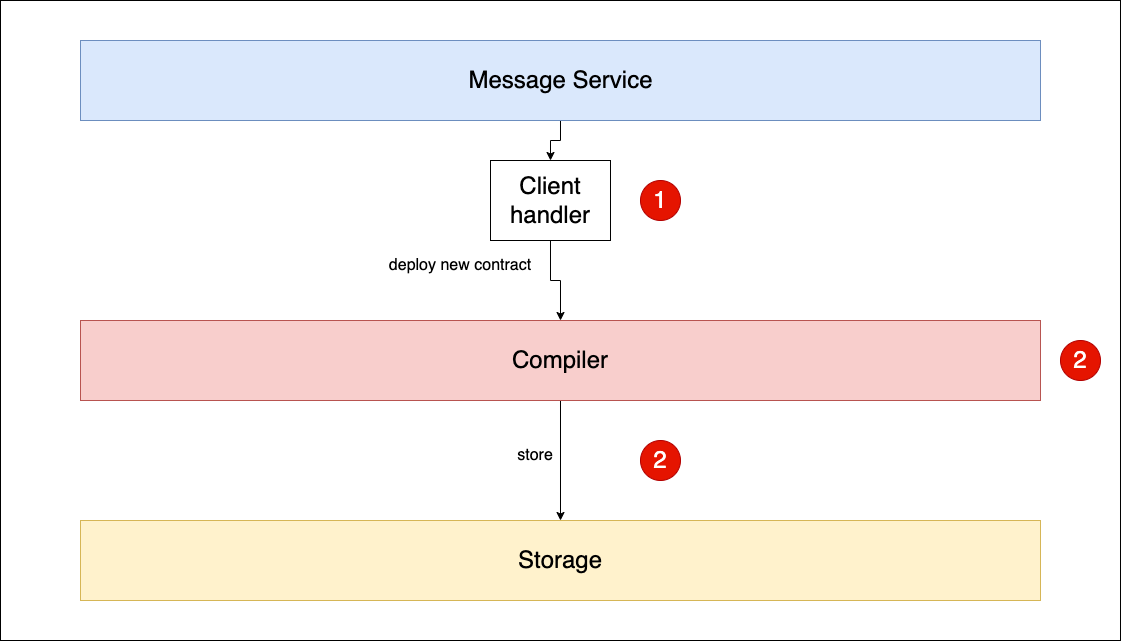
\includegraphics[width=0.9\textwidth]{immagini/capitolo-5/deploy-contract-flow.png}
		\caption{New contract upload execution flow.}
		\label{fig:deploy-contract-flow}
	\end{center}
\end{figure}

The flow for \textit{deploy} a new contract is illustrated in figure \ref{fig:deploy-contract-flow}. The 
request is received by the \verb|MessageService| and via the \verb|ClientHandler| the request is directed 
to the compiler (\textbf{1}). The contract is compiled and if the compilation returns no errors 
(\textbf{2}), it stores the contract and the compiled in the \textit{Storage} module (\textbf{3}).

Request to the server for contract deployment:
{
  \small
  \begin{Verbatim}[numbers=left,xleftmargin=1cm,firstnumber=1,breaklines=true,breakanywhere=true,tabsize=2]
    {
      "message": {
        "sourceCode": "stipula SwapAsset {\n    asset assetA:stipula_assetA_ed8i9wk, assetB:stipula_assetB_pl1n5cc\n    field amountAssetA, amountAssetB\n    init Inactive\n\n    agreement (Alice, Bob)(amountAssetA, amountAssetB) {\n        Alice, Bob: amountAssetA, amountAssetB\n    } ==> @Inactive\n\n    @Inactive Alice : depositAssetA()[y]\n        (y == amountAssetA) {\n            y -o assetA;\n            _\n    } ==> @Swap\n\n    @Swap Bob : depositAssetBAndSwap()[y]\n        (y == amountAssetB) {\n            y -o assetB\n            assetB -o Alice\n            assetA -o Bob;\n            _\n    } ==> @End\n}",
        "type": "DeployContract"
      },
      "signatures": {
        "MIGfMA0GCSqGSIb3DQEBAQUAA4GNADCBiQKBgQCo/GjVKS+3gAA55+kko41yINdOcCLQMSBQyuTTkKHE1mhu/TgOpivM0wLPsSga8hQMr3+v3aR0IF/vfCRf6SdiXmWx/jflmEXtnT6fkGcnV6dGNUpHWXSpwUIDt0N88jfnEqekx4S+KDCKg99sGEeHeT65fKS8lB0gjHMt9AOriwIDAQAB": "V5gJHSax5J5nWYZlyhJr+RdJhbWrog9/urvyfWPTNWf6jkLRT16xAdLYBR1NucOmKTf9iW6mVMVpUxtrGPXktTUEIzxJpp81jR06hDBUpH0Eu6pkiw9nomTUZvuCX9DR/+WOSBz0jMO5lOznl6At3OP1mXsgNyRtPJTi2q4yHs0="
      }
    }
  \end{Verbatim}
}

Server response:
{
  \small
  \begin{Verbatim}[numbers=left,xleftmargin=1cm,firstnumber=1,breaklines=true,breakanywhere=true,tabsize=2]
    {
      "data": "d50ed1a3-7a65-4238-867e-df48536b7243",
      "statusCode": 200,
      "statusMessage": "Success",
      "type": "SuccessDataResponse"
    }
  \end{Verbatim}
}

The value in the \verb|data| field indicates the identifier of the deployed contract.

\paragraph{Single-use-seals by Alice}

{
  \small
  \begin{figure}[htbp]
    \begin{center}
      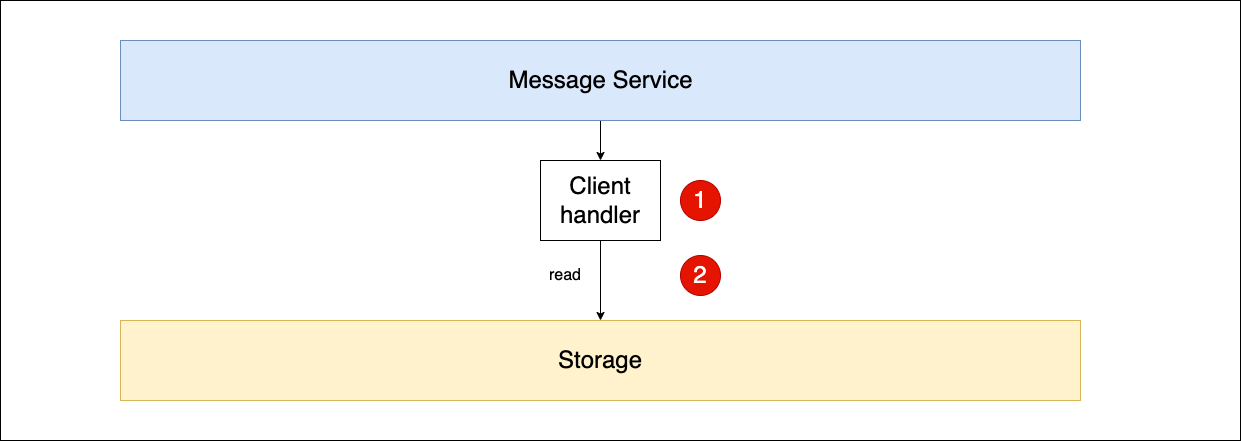
\includegraphics[width=0.9\textwidth]{immagini/capitolo-5/get-funds-flow.png}
      \caption{Execution flow for Alice's funds read request.}
      \label{fig:get-funds-flow}
    \end{center}
  \end{figure}
}

The description of the following flow is illustrated in figure \ref{fig:get-funds-flow}. When a user wants 
to know the available funds associated with his address, the user sends a particular message (\textbf{1}). 
The request is directed to the \textit{Storage} module (\textbf{2}) and the availability of funds is sent 
to the user in response.

Request to the server to get the single-use-seals in Alice's possession:
{
  \small
  \begin{Verbatim}[numbers=left,xleftmargin=1cm,firstnumber=1,breaklines=true,breakanywhere=true,tabsize=2]
    {
      "message": {
        "address": "ubL35Am7TimL5R4oMwm2OxgAYA3XT3BeeDE56oxqdLc=",
        "type": "GetOwnershipsByAddress"
      },
      "signatures": {
        "MIGfMA0GCSqGSIb3DQEBAQUAA4GNADCBiQKBgQCo/GjVKS+3gAA55+kko41yINdOcCLQMSBQyuTTkKHE1mhu/TgOpivM0wLPsSga8hQMr3+v3aR0IF/vfCRf6SdiXmWx/jflmEXtnT6fkGcnV6dGNUpHWXSpwUIDt0N88jfnEqekx4S+KDCKg99sGEeHeT65fKS8lB0gjHMt9AOriwIDAQAB": "MomZTc63z7PfH35c1dL4tjXebcsW+0Zxl0nP1NQdcUFws98DX+bMWI7L0C6IO5lxvkYve4zdio1Crn97FXvngK4aVfiEZEnHOJ0tstq7uQYGErM3DDAABqPq8HH5yoKnLST2LWpO0oD8G/VXvIE6qMT5D34W1Ci0q4uh+7y3EcY="
      }
    }
  \end{Verbatim}
}

Server response:
{
  \small
  \begin{Verbatim}[numbers=left,xleftmargin=1cm,firstnumber=1,breaklines=true,breakanywhere=true,tabsize=2]
    {
      "data": "[
          Ownership{
            id='2b4a4614-3bb4-4554-93fe-c034c3ba5a9c', 
            singleUseSeal=SingleUseSeal{
              assetId='stipula_assetA_ed8i9wk', 
              amount=RealType{
                value=1400, 
                decimals=2
              }, 
              lockScript='DUP\nSHA256\nPUSH str ubL35Am7TimL5R4oMwm2OxgAYA3XT3BeeDE56oxqdLc=\nEQUAL\nCHECKSIG\nHALT\n'
            }, 
            unlockScript='', 
            contractInstanceId=''
          }
        ]",
      "statusCode": 200,
      "statusMessage": "Success",
      "type": "SuccessDataResponse"
    }
  \end{Verbatim}
}

\paragraph{Single-use-seals by Bob}

Server request to get Bob's single-use-seals:
{
  \small
  \begin{Verbatim}[numbers=left,xleftmargin=1cm,firstnumber=1,breaklines=true,breakanywhere=true,tabsize=2]
    {
      "message": {
        "address": "f3hVW1Amltnqe3KvOT00eT7AU23FAUKdgmCluZB+nss=",
        "type": "GetOwnershipsByAddress"
      },
      "signatures": {
        "MIGfMA0GCSqGSIb3DQEBAQUAA4GNADCBiQKBgQDErzzgD2ZslZxciFAiX3/ot7lrkZDw4148jFZrsDZPE6CVs9xXFSHGgy/mFvIFLXhnChO6Nyd2be3lbgeavLMCMVUiTStXr117Km17keWpb3sItkKKsLFBOcIIU8XXowI/OhzQN2XPZYESHgjdQ5vwEj2YyueiS7WKP94YWz/pswIDAQAB": "hSNodnUyusffNlv+KNq4605pFvqh91pVspFhTgbmWccE/LKM6h4bedpvTgMHoVDezvA7v2XTzmLG5eL3lOeA6I2xJMH32DcV60IPSoh61oVHnwPQcQHY039D4y5VSJ0GMQJKIcTEq3fqIdabg7261xUaegHUnXrcyynh9GpMJxk="
      }
    }
  \end{Verbatim}
}

Server response:
{
  \small
  \begin{Verbatim}[numbers=left,xleftmargin=1cm,firstnumber=1,breaklines=true,breakanywhere=true,tabsize=2]
    {
      "data": "[
          Ownership{
            id='7a19f50e-eae9-461d-bd58-9946ea39ccf0', 
            singleUseSeal=SingleUseSeal{
              assetId='stipula_assetB_pl1n5cc', 
              amount=RealType{
                value=1100, 
                decimals=2
              }, 
              lockScript='DUP\nSHA256\nPUSH str f3hVW1Amltnqe3KvOT00eT7AU23FAUKdgmCluZB+nss=\nEQUAL\nCHECKSIG\nHALT\n'
            }, 
            unlockScript='', 
            contractInstanceId=''
          }
        ]",
      "statusCode": 200,
      "statusMessage": "Success",
      "type": "SuccessDataResponse"
    }
  \end{Verbatim}
}

\paragraph{Agreement}

The description of the following flow is illustrated in figure \ref{fig:contract-flow}. When users have 
agreed to execute an agreement, an \verb|AgreementCall| message is sent (see 
\ref{agreement-call-message}). This request is placed in the request queue (\textbf{1.1} and 
\textbf{1.2}). The virtual machine dequeues the request (\textbf{2}) and the function \textit{agreement} 
(\textbf{4}) is executed. Once the execution of the function has finished without errors, the result of 
the processing will be stored in the \textit{Storage} module (\textbf{5}) and finally the virtual machine 
will notify the client of the success of the operation (\textbf{ 6}).

Request to the server to make the \verb|agreement| function call:
{
  \small
  \begin{Verbatim}[numbers=left,xleftmargin=1cm,firstnumber=1,breaklines=true,breakanywhere=true,tabsize=2]
    {
      "message": {
        "contractId": "d50ed1a3-7a65-4238-867e-df48536b7243",
        "arguments": [
          {
            "argument": {
              "first": "real",
              "second": "amountAssetA",
              "third": "1400 2"
            }
          },
          {
            "argument": {
              "first": "real",
              "second": "amountAssetB",
              "third": "1100 2"
            }
          }
        ],
        "parties": {
          "Bob": {
            "address": "f3hVW1Amltnqe3KvOT00eT7AU23FAUKdgmCluZB+nss=",
            "publicKey": "MIGfMA0GCSqGSIb3DQEBAQUAA4GNADCBiQKBgQDErzzgD2ZslZxciFAiX3/ot7lrkZDw4148jFZrsDZPE6CVs9xXFSHGgy/mFvIFLXhnChO6Nyd2be3lbgeavLMCMVUiTStXr117Km17keWpb3sItkKKsLFBOcIIU8XXowI/OhzQN2XPZYESHgjdQ5vwEj2YyueiS7WKP94YWz/pswIDAQAB"
          },
          "Alice": {
            "address": "ubL35Am7TimL5R4oMwm2OxgAYA3XT3BeeDE56oxqdLc=",
            "publicKey": "MIGfMA0GCSqGSIb3DQEBAQUAA4GNADCBiQKBgQCo/GjVKS+3gAA55+kko41yINdOcCLQMSBQyuTTkKHE1mhu/TgOpivM0wLPsSga8hQMr3+v3aR0IF/vfCRf6SdiXmWx/jflmEXtnT6fkGcnV6dGNUpHWXSpwUIDt0N88jfnEqekx4S+KDCKg99sGEeHeT65fKS8lB0gjHMt9AOriwIDAQAB"
          }
        },
        "type": "AgreementCall"
      },
      "signatures": {
        "MIGfMA0GCSqGSIb3DQEBAQUAA4GNADCBiQKBgQDErzzgD2ZslZxciFAiX3/ot7lrkZDw4148jFZrsDZPE6CVs9xXFSHGgy/mFvIFLXhnChO6Nyd2be3lbgeavLMCMVUiTStXr117Km17keWpb3sItkKKsLFBOcIIU8XXowI/OhzQN2XPZYESHgjdQ5vwEj2YyueiS7WKP94YWz/pswIDAQAB": "crMKGFVc5QYmYfbyxDaqhXEi0/GRO+j2OD8HtBbysVm1/+2D+nFATAOvm+LbDtLMMBHxTE8a4JHzMN1DZ1uokkwHKyv80/IVMLwjZi6RFl1Jk7jUpUq6nBCPfqfa7u2IKtzv0joJXR/8BNyN3u6+PReS+4N530+ESN3W2P3tIFk=",
        "MIGfMA0GCSqGSIb3DQEBAQUAA4GNADCBiQKBgQCo/GjVKS+3gAA55+kko41yINdOcCLQMSBQyuTTkKHE1mhu/TgOpivM0wLPsSga8hQMr3+v3aR0IF/vfCRf6SdiXmWx/jflmEXtnT6fkGcnV6dGNUpHWXSpwUIDt0N88jfnEqekx4S+KDCKg99sGEeHeT65fKS8lB0gjHMt9AOriwIDAQAB": "OK9fuuEHTIV5gjtghgvFqsJZI98Ip7IYXvph0J79kTwfRVvJnH5mX9Rs/lDUWnznOmY3HTADwn4QgzMQgdu+qAfixoyJWvZJZ8XjNo/N1YI3nnaaXhvkpR80SHhxqhFLfET6rAx5qXpziOZS7NfcIasn6Lj35hbQCfcjKvxf76w="
      }
    }
  \end{Verbatim}
}

Server response:
{
  \small
  \begin{Verbatim}[numbers=left,xleftmargin=1cm,firstnumber=1,breaklines=true,breakanywhere=true,tabsize=2]
    {
      "data": "e9cbb96e-4d20-47d2-80e6-5b56701800b1",
      "statusCode": 200,
      "statusMessage": "Success",
      "type": "SuccessDataResponse"
    }
  \end{Verbatim}
}

The value in the \verb|data| field indicates the identifier of the created contract instance.

\paragraph{depositAssetA call}

In this function Alice has to make a \textit{Pay-to-Contract}. Compared to the description of the previous 
flow, before the \textit{Legal Contract Virtual Machine} executes the function, it is necessary to check 
that the \textit{single-use-seal} sent by Alice actually belongs to Alice and is of the quantity requested 
by the instance of the contract. To do this, it is necessary to carry out these checks with the 
\textit{Script Virtual Machine} (see point \textbf{3} of figure \ref{fig:contract-flow}). Once these 
checks have been completed, the virtual machine will be able to proceed with the execution of the 
function requested by Alice.

Request to the server to make the \verb|depositAssetA| function call:
{
  \small
  \begin{Verbatim}[numbers=left,xleftmargin=1cm,firstnumber=1,breaklines=true,breakanywhere=true,tabsize=2]
    {
      "message": {
        "contractInstanceId": "e9cbb96e-4d20-47d2-80e6-5b56701800b1",
        "functionName": "depositAssetA",
        "arguments": [
          {
            "argument": {
              "first": "asset",
              "second": "y",
              "third": {
                "ownershipId": "2b4a4614-3bb4-4554-93fe-c034c3ba5a9c",
                "address": "ubL35Am7TimL5R4oMwm2OxgAYA3XT3BeeDE56oxqdLc=",
                "unlockScript": "PUSH str PLjodnT+m3RNIitQAPBDCsRmJPHCqrwZOY/CPiHFZGnl+DRN6soqxMy3ehTFaUwxBjjf7qfBfvTDq5oBItTFrtz1Rn5SDS1ybdbkwpKaOXVglNOw7ZEG9bbZ1mo1oA7IAjRiIilzUetCstE5rPZIf9XOXr/RQ5AHkZUn2CztsvA=\nPUSH str MIGfMA0GCSqGSIb3DQEBAQUAA4GNADCBiQKBgQCo/GjVKS+3gAA55+kko41yINdOcCLQMSBQyuTTkKHE1mhu/TgOpivM0wLPsSga8hQMr3+v3aR0IF/vfCRf6SdiXmWx/jflmEXtnT6fkGcnV6dGNUpHWXSpwUIDt0N88jfnEqekx4S+KDCKg99sGEeHeT65fKS8lB0gjHMt9AOriwIDAQAB\n"
              }
            }
          }
        ],
        "type": "FunctionCall"
      },
      "signatures": {   
        "MIGfMA0GCSqGSIb3DQEBAQUAA4GNADCBiQKBgQCo/GjVKS+3gAA55+kko41yINdOcCLQMSBQyuTTkKHE1mhu/TgOpivM0wLPsSga8hQMr3+v3aR0IF/vfCRf6SdiXmWx/jflmEXtnT6fkGcnV6dGNUpHWXSpwUIDt0N88jfnEqekx4S+KDCKg99sGEeHeT65fKS8lB0gjHMt9AOriwIDAQAB": "MVm0fv9zBntC7ElPhNYaISpgmOdCh8blRsvkU2gtulbWQvwg/CuKtcOIHxakTrffnrW7iw/KLB0n46HulBL6KAcl02U9HSt0+YwX3imJ50QVWU7kmLoMy5d8uQ+seZzXifsaf7OvE1OpAWXNwh7ICsRZv9U6aV39c13SUqwHjTs="
      }
    }
  \end{Verbatim}
}

Server response:
{
  \small
  \begin{Verbatim}[numbers=left,xleftmargin=1cm,firstnumber=1,breaklines=true,breakanywhere=true,tabsize=2]
    {
      "statusCode": 200,
      "statusMessage": "Success",
      "type": "SuccessDataResponse"
    }
  \end{Verbatim}
}

\paragraph{depositAssetBAndSwap call}

Request to the server to make the \verb|depositAssetBAndSwap| function call:
{
  \small
  \begin{Verbatim}[numbers=left,xleftmargin=1cm,firstnumber=1,breaklines=true,breakanywhere=true,tabsize=2]
    {
      "message": {
        "contractInstanceId": "e9cbb96e-4d20-47d2-80e6-5b56701800b1",
        "functionName": "depositAssetBAndSwap",
        "arguments": [
          {
            "argument": {
              "first": "asset",
              "second": "y",
              "third": {
                "ownershipId": "7a19f50e-eae9-461d-bd58-9946ea39ccf0",
                "address": "f3hVW1Amltnqe3KvOT00eT7AU23FAUKdgmCluZB+nss=",
                "unlockScript": "PUSH str Q0bPh9lThyrg1slz9AGDJDJh1BecN9SlGCeVe3BqLod+zO7q0wvIy8tLognHNBkR8e8zKo6nWGQ8qZ7egjOmm5BQsqZzt8xL3gBbR36vgk9J3G9ObiTR2Dd7hMqsqyJnLT3aZUPXGc6RZoM/iUFGJUXhq2T6DStvYNKuAH+Lfow=\nPUSH str MIGfMA0GCSqGSIb3DQEBAQUAA4GNADCBiQKBgQDErzzgD2ZslZxciFAiX3/ot7lrkZDw4148jFZrsDZPE6CVs9xXFSHGgy/mFvIFLXhnChO6Nyd2be3lbgeavLMCMVUiTStXr117Km17keWpb3sItkKKsLFBOcIIU8XXowI/OhzQN2XPZYESHgjdQ5vwEj2YyueiS7WKP94YWz/pswIDAQAB\n"
              }
            }
          }
        ],
        "type": "FunctionCall"
      },
      "signatures": {
        "MIGfMA0GCSqGSIb3DQEBAQUAA4GNADCBiQKBgQDErzzgD2ZslZxciFAiX3/ot7lrkZDw4148jFZrsDZPE6CVs9xXFSHGgy/mFvIFLXhnChO6Nyd2be3lbgeavLMCMVUiTStXr117Km17keWpb3sItkKKsLFBOcIIU8XXowI/OhzQN2XPZYESHgjdQ5vwEj2YyueiS7WKP94YWz/pswIDAQAB": "kh7JupouiEdeLuilXUdoJqAuPVx28JTg9dySp/ZNJGD5+XW8YhhIgiMJYOhGeN6DJTj/x+TmC96uyS8IwssUt/Hulnh2OAZzkc3FljWj1k/XfL0yye95u+YBxg+t8AddQBi+4uA4yOdzb8YdrONlzGu7t0roirmO8SbOqQR1uX8="
      }
    }
  \end{Verbatim}
}

Server response:
{
  \small
  \begin{Verbatim}[numbers=left,xleftmargin=1cm,firstnumber=1,breaklines=true,breakanywhere=true,tabsize=2]
    {
      "statusCode": 200,
      "statusMessage": "Success",
      "type": "SuccessDataResponse"
    }
  \end{Verbatim}
}

\paragraph{Single-use-seals by Alice}

Server request to get Alice's single-use-seals:
{
  \small
  \begin{Verbatim}[numbers=left,xleftmargin=1cm,firstnumber=1,breaklines=true,breakanywhere=true,tabsize=2]
    {
      "message": {
        "address": "ubL35Am7TimL5R4oMwm2OxgAYA3XT3BeeDE56oxqdLc=",
        "type": "GetOwnershipsByAddress"
      },
      "signatures": {
        "MIGfMA0GCSqGSIb3DQEBAQUAA4GNADCBiQKBgQCo/GjVKS+3gAA55+kko41yINdOcCLQMSBQyuTTkKHE1mhu/TgOpivM0wLPsSga8hQMr3+v3aR0IF/vfCRf6SdiXmWx/jflmEXtnT6fkGcnV6dGNUpHWXSpwUIDt0N88jfnEqekx4S+KDCKg99sGEeHeT65fKS8lB0gjHMt9AOriwIDAQAB": "MomZTc63z7PfH35c1dL4tjXebcsW+0Zxl0nP1NQdcUFws98DX+bMWI7L0C6IO5lxvkYve4zdio1Crn97FXvngK4aVfiEZEnHOJ0tstq7uQYGErM3DDAABqPq8HH5yoKnLST2LWpO0oD8G/VXvIE6qMT5D34W1Ci0q4uh+7y3EcY="
      }
    }
  \end{Verbatim}
}

Server response:
{
  \small
  \begin{Verbatim}[numbers=left,xleftmargin=1cm,firstnumber=1,breaklines=true,breakanywhere=true,tabsize=2]
    {
      "data": "[
          Ownership{
            id='2b4a4614-3bb4-4554-93fe-c034c3ba5a9c', 
            singleUseSeal=SingleUseSeal{
              assetId='stipula_assetA_ed8i9wk', 
              amount=RealType{
                value=1400, 
                decimals=2
              }, 
              lockScript='DUP\nSHA256\nPUSH str ubL35Am7TimL5R4oMwm2OxgAYA3XT3BeeDE56oxqdLc=\nEQUAL\nCHECKSIG\nHALT\n'
            }, 
            unlockScript='PUSH str PLjodnT+m3RNIitQAPBDCsRmJPHCqrwZOY/CPiHFZGnl+DRN6soqxMy3ehTFaUwxBjjf7qfBfvTDq5oBItTFrtz1Rn5SDS1ybdbkwpKaOXVglNOw7ZEG9bbZ1mo1oA7IAjRiIilzUetCstE5rPZIf9XOXr/RQ5AHkZUn2CztsvA=\nPUSH str MIGfMA0GCSqGSIb3DQEBAQUAA4GNADCBiQKBgQCo/GjVKS+3gAA55+kko41yINdOcCLQMSBQyuTTkKHE1mhu/TgOpivM0wLPsSga8hQMr3+v3aR0IF/vfCRf6SdiXmWx/jflmEXtnT6fkGcnV6dGNUpHWXSpwUIDt0N88jfnEqekx4S+KDCKg99sGEeHeT65fKS8lB0gjHMt9AOriwIDAQAB\n', 
            contractInstanceId='e9cbb96e-4d20-47d2-80e6-5b56701800b1'
          }, 
          Ownership{
            id='4cbec85d-f17e-4928-a029-7cf0e646a3f6', 
            singleUseSeal=SingleUseSeal{
              assetId='stipula_assetB_pl1n5cc', 
              amount=RealType{
                value=100, 
                decimals=2
              }, 
              lockScript='DUP\nSHA256\nPUSH str ubL35Am7TimL5R4oMwm2OxgAYA3XT3BeeDE56oxqdLc=\nEQUAL\nCHECKSIG\nHALT\n'
            }, 
            unlockScript='', 
            contractInstanceId=''
          }
        ]",
      "statusCode": 200,
      "statusMessage": "Success",
      "type": "SuccessDataResponse"
    }
  \end{Verbatim}
}

It is possible to see that the first single-use-seal has been spent and that's what was deposited in the 
contract instance. Evidence that the funds have been spent is given by the \verb|unlockScript| field. 
While, the second single-use-seal represents the asset that was in Bob's possession.

\paragraph{Single-use-seals by Bob}

Server request to get Bob's single-use-seals:
{
  \small
  \begin{Verbatim}[numbers=left,xleftmargin=1cm,firstnumber=1,breaklines=true,breakanywhere=true,tabsize=2]
    {
      "message": {
        "address": "f3hVW1Amltnqe3KvOT00eT7AU23FAUKdgmCluZB+nss=",
        "type": "GetOwnershipsByAddress"
      },
      "signatures": {
        "MIGfMA0GCSqGSIb3DQEBAQUAA4GNADCBiQKBgQDErzzgD2ZslZxciFAiX3/ot7lrkZDw4148jFZrsDZPE6CVs9xXFSHGgy/mFvIFLXhnChO6Nyd2be3lbgeavLMCMVUiTStXr117Km17keWpb3sItkKKsLFBOcIIU8XXowI/OhzQN2XPZYESHgjdQ5vwEj2YyueiS7WKP94YWz/pswIDAQAB": "hSNodnUyusffNlv+KNq4605pFvqh91pVspFhTgbmWccE/LKM6h4bedpvTgMHoVDezvA7v2XTzmLG5eL3lOeA6I2xJMH32DcV60IPSoh61oVHnwPQcQHY039D4y5VSJ0GMQJKIcTEq3fqIdabg7261xUaegHUnXrcyynh9GpMJxk="
      }
    }
  \end{Verbatim}
}

Server response:
{
  \small
  \begin{Verbatim}[numbers=left,xleftmargin=1cm,firstnumber=1,breaklines=true,breakanywhere=true,tabsize=2]
    {
      "data": "[
          Ownership{
            id='7a19f50e-eae9-461d-bd58-9946ea39ccf0', 
            singleUseSeal=SingleUseSeal{
              assetId='stipula_assetB_pl1n5cc', 
              amount=RealType{
                value=1100, 
                decimals=2
              }, 
              lockScript='DUP\nSHA256\nPUSH str f3hVW1Amltnqe3KvOT00eT7AU23FAUKdgmCluZB+nss=\nEQUAL\nCHECKSIG\nHALT\n'
            }, 
            unlockScript='PUSH str Q0bPh9lThyrg1slz9AGDJDJh1BecN9SlGCeVe3BqLod+zO7q0wvIy8tLognHNBkR8e8zKo6nWGQ8qZ7egjOmm5BQsqZzt8xL3gBbR36vgk9J3G9ObiTR2Dd7hMqsqyJnLT3aZUPXGc6RZoM/iUFGJUXhq2T6DStvYNKuAH+Lfow=\nPUSH str MIGfMA0GCSqGSIb3DQEBAQUAA4GNADCBiQKBgQDErzzgD2ZslZxciFAiX3/ot7lrkZDw4148jFZrsDZPE6CVs9xXFSHGgy/mFvIFLXhnChO6Nyd2be3lbgeavLMCMVUiTStXr117Km17keWpb3sItkKKsLFBOcIIU8XXowI/OhzQN2XPZYESHgjdQ5vwEj2YyueiS7WKP94YWz/pswIDAQAB\n', 
            contractInstanceId='e9cbb96e-4d20-47d2-80e6-5b56701800b1'
          }, 
          Ownership{
            id='bd1f5959-cd8d-4716-8ece-19e1757c6ac2', 
            singleUseSeal=SingleUseSeal{
              assetId='stipula_assetA_ed8i9wk', 
              amount=RealType{
                value=100, 
                decimals=2
              }, 
              lockScript='DUP\nSHA256\nPUSH str f3hVW1Amltnqe3KvOT00eT7AU23FAUKdgmCluZB+nss=\nEQUAL\nCHECKSIG\nHALT\n'
            }, 
            unlockScript='', 
            contractInstanceId=''
          }
        ]",
      "statusCode": 200,
      "statusMessage": "Success",
      "type": "SuccessDataResponse"
    }
  \end{Verbatim}
}

It is possible to see that the first single-use-seal has been spent and that's what was deposited in the contract 
instance. Evidence that the funds have been spent is given by the \verb|unlockScript| field. While, the 
second single-use-seal represents the asset that was in Alice's possession.

\subsection{Asset swap with scheduled event}

The complete code is present in the appendix \ref{app:asset-swap-event-complete-code}. The 
\textit{Stipula} code compared to the previous version does not change much. The only changes made are:
\begin{enumerate}
  \item Line 3: A new global variable \verb|waitTimeBeforeSwapping| is defined. This variable indicates 
  the time needed to wait before being able to swap assets. It is a value that is agreed between the 
  participants of the \textit{agreement} contract;
  \item Lines 6 and 7: it is specified that a value for \verb|waitTimeBeforeSwapping| must be supplied 
  during the \textit{agreement} phase;
  \item Line 14: the state the contract instance will go to once the function is executed 
  \verb|depositAssetA| will exit without errors, it is no longer \verb|@Swap| but \verb|@Deposit|;
  \item Line 16: if Bob wants to deposit his asset, the contract instance must be in the \verb|@Deposit| 
  and no longer \verb|@Swap|. Also, the function name changes from \verb|depositAssetBAndSwap| to 
  \verb|depositAssetB|;
  \item From line 19 to line 23: the code that encodes the \textit{obligation} that will have to be 
  executed at the time indicated in line 19 is defined, that is, an event will be scheduled that will 
  execute the obligation at the time \verb|now + waitTimeBeforeSwapping|;
  \item Line 24: the state the contract instance will go to once the \verb|depositAssetB| will exit 
  without errors, it is no longer \verb|@End| but \verb|@Swap|;
  \item Line 20: in order to execute the obligation at the defined time, the status of the contract 
  instance must be \verb|@Swap|;
  \item Line 23: the state in which the contract instance will go once the execution of the obligation 
  has finished without errors, will be \verb|@End|.
\end{enumerate}

The bytecode is almost similar to the one produced for the previous example, the substantial change 
occurs for the encoding of the \textit{obligation}. In particular:
\begin{enumerate}
  \item Lines 58 to 60: This piece of code is part of the \verb|depositAssetB| function. These specific 
  lines allow to calculate the \textit{absolute} time, necessary to schedule an \textit{event}, which will 
  carry out a particular function call. To indicate where the function code to be executed by the event 
  begins, the \verb|TRIGGER obligation_1| instruction is used. Once the execution of the function is 
  finished, the event will be scheduled and when the time $t$ arrives, the \verb|EventTrigger| will put 
  the request in the request queue (see \ref{execution-flow-for-obligation});
  \item Line 64 to line 75: lines 66 to 75 correspond exactly to lines 55 to 64 of the previous function. 
  However, this code is now part of a particular function, whose signature is defined on line 64. Indeed, 
  it specifies: this code encodes a \textit{obligation} (\verb|obligation|); in order to perform this 
  obligation, the state of the contract instance must be \verb|@Swap|; the name of the function 
  \verb|obligation_1|; the state in which the contract instance will go once the execution of the 
  obligation has finished without errors, will be \verb|@End|.
\end{enumerate}

\subsubsection{Example of execution}

An example of execution of this contract is illustrated in the appendix 
\ref{app:asset-swap-event-complete-execution}. Only a few steps will be shown in this section.

\paragraph{Agreement}

The \textit{agreement} phase is very similar to the previous example, the only change is to set the value 
to the variable \verb|waitTimeBeforeSwapping|.

Request to the server to make the \verb|agreement| function call:
{
  \small
  \begin{Verbatim}[numbers=left,xleftmargin=1cm,firstnumber=1,breaklines=true,breakanywhere=true,tabsize=2]
    {
      "message": {
        "contractId": "79caadf1-abbe-418a-a9a2-bd132a6f3e9e",
        "arguments": [
          {
            "argument": {
              "first": "real",
              "second": "amountAssetA",
              "third": "1400 2"
            }
          },
          {
            "argument": {
              "first": "real",
              "second": "amountAssetB",
              "third": "1100 2"
            }
          },
          {
            "argument": {
              "first": "time",
              "second": "waitTimeBeforeSwapping",
              "third": "100"
            }
          }
        ],
        "parties": {
          "Bob": {
            "address": "f3hVW1Amltnqe3KvOT00eT7AU23FAUKdgmCluZB+nss=",
            "publicKey": "MIGfMA0GCSqGSIb3DQEBAQUAA4GNADCBiQKBgQDErzzgD2ZslZxciFAiX3/ot7lrkZDw4148jFZrsDZPE6CVs9xXFSHGgy/mFvIFLXhnChO6Nyd2be3lbgeavLMCMVUiTStXr117Km17keWpb3sItkKKsLFBOcIIU8XXowI/OhzQN2XPZYESHgjdQ5vwEj2YyueiS7WKP94YWz/pswIDAQAB"
          },
          "Alice": {
            "address": "ubL35Am7TimL5R4oMwm2OxgAYA3XT3BeeDE56oxqdLc=",
            "publicKey": "MIGfMA0GCSqGSIb3DQEBAQUAA4GNADCBiQKBgQCo/GjVKS+3gAA55+kko41yINdOcCLQMSBQyuTTkKHE1mhu/TgOpivM0wLPsSga8hQMr3+v3aR0IF/vfCRf6SdiXmWx/jflmEXtnT6fkGcnV6dGNUpHWXSpwUIDt0N88jfnEqekx4S+KDCKg99sGEeHeT65fKS8lB0gjHMt9AOriwIDAQAB"
          }
        },
        "type": "AgreementCall"
      },
      "signatures": {
        "MIGfMA0GCSqGSIb3DQEBAQUAA4GNADCBiQKBgQDErzzgD2ZslZxciFAiX3/ot7lrkZDw4148jFZrsDZPE6CVs9xXFSHGgy/mFvIFLXhnChO6Nyd2be3lbgeavLMCMVUiTStXr117Km17keWpb3sItkKKsLFBOcIIU8XXowI/OhzQN2XPZYESHgjdQ5vwEj2YyueiS7WKP94YWz/pswIDAQAB": "Wrqyz5udZAGarLbSlxhYD+Ur6+EqTCFiwqBHEL2IsO5Y23Yxv14O3UzknrwK41L5LPUgVxR3K75AAZ4n+UcUdDNHlm9KHN7rqpsbe7v3yK2q8Qkk6c4IYNPDRFy3Zw62HH94O7tx8CzcvRfdX4fi+RItf4Fa7hb8Ui/crxDEQN8=",
        "MIGfMA0GCSqGSIb3DQEBAQUAA4GNADCBiQKBgQCo/GjVKS+3gAA55+kko41yINdOcCLQMSBQyuTTkKHE1mhu/TgOpivM0wLPsSga8hQMr3+v3aR0IF/vfCRf6SdiXmWx/jflmEXtnT6fkGcnV6dGNUpHWXSpwUIDt0N88jfnEqekx4S+KDCKg99sGEeHeT65fKS8lB0gjHMt9AOriwIDAQAB": "o/bdsudfHdR4BBd9EVaGYikksIezSEdwhHELH/f7xRD9g4uokO5g8wHph6LOht5dt9Y+dYt+Qrt+zNZzGUP8a50R7WB2gNz0Jn3zndKnVoBVhsda/zEwIA2pqccP2Sda7zCYiFTfgnmlUZZZfxjtLazBUzDE/vVVFcwtXAHYMXk="
      }
    }
  \end{Verbatim}
}

For simplicity, the value for \verb|waitTimeBeforeSwapping| is equal to 100, that is, after Bob deposits 
his asset, they will wait 100 seconds before exchanging assets.

Server response:
{
  \small
  \begin{Verbatim}[numbers=left,xleftmargin=1cm,firstnumber=1,breaklines=true,breakanywhere=true,tabsize=2]
    {
      "data": "48819afd-e28f-4037-82fd-1d073ee1d318",
      "statusCode": 200,
      "statusMessage": "Success",
      "type": "SuccessDataResponse"
    }
  \end{Verbatim}
}

The value in the \verb|data| field indicates the identifier of the created contract instance.

\paragraph{Event trigger and execution of the obligation}

The call of \verb|depositAssetA| and \verb|depositAssetB| are the same as the previous example. 

From the server logs it can be seen that the event was triggered, the code encoding the obligation was 
loaded and executed:
{
  \small
  \begin{Verbatim}[numbers=left,xleftmargin=1cm,firstnumber=1,breaklines=true,breakanywhere=true,tabsize=2]
    EventTrigger: A new scheduled request has been triggered => EventTriggerSchedulingRequest{
      request=CreateEventRequest{
        obligationFunctionName='obligation_1', 
        time=1680032647
      }, 
      contractId='79caadf1-abbe-418a-a9a2-bd132a6f3e9e', 
      contractInstanceId='48819afd-e28f-4037-82fd-1d073ee1d318'
    }
    EventTrigger: Enqueuing the request...
    EventTrigger: Notifying the virtual machine...
    EventTrigger: Virtual machine notified
    EventTrigger: Removing the request from EventTriggerHandler...
    VirtualMachine: Ready to dequeue a value...
    VirtualMachine: Request received => Pair{
      first=null, 
      second=EventTriggerSchedulingRequest{
        request=CreateEventRequest{
          obligationFunctionName='obligation_1', 
          time=1680032647
        }, 
        contractId='79caadf1-abbe-418a-a9a2-bd132a6f3e9e', 
        contractInstanceId='48819afd-e28f-4037-82fd-1d073ee1d318'
      }
    }
    VirtualMachine: Just received a trigger request
    loadObligationFunction: Loading the obligation function...
    loadObligationFunction: Obligation function loaded
    VirtualMachine: Function
    start:
    PUSH real 100 2
    GLOAD assetB
    GLOAD Alice
    WITHDRAW assetB
    PUSH real 100 2
    GLOAD assetA
    GLOAD Bob
    WITHDRAW assetA
    end:
    HALT
  
    loadBytecode: Loading the bytecode...
    loadBytecode: Bytecode loaded
  
    VirtualMachine: loadBytecode
    start:
    PUSH real 100 2
    GLOAD assetB
    GLOAD Alice
    WITHDRAW assetB
    PUSH real 100 2
    GLOAD assetA
    GLOAD Bob
    WITHDRAW assetA
    end:
    HALT
  
    LegalContractVirtualMachine: execute => Final state of the execution below
    LegalContractVirtualMachine: execute => The stack is empty
  
    LegalContractVirtualMachine: execute => GlobalSpace
    assetA: 13.00 stipula_assetA_ed8i9wk, changed: true
    amountAssetA: 14.00, changed: false
    assetB: 10.00 stipula_assetB_pl1n5cc, changed: true
    amountAssetB: 11.00, changed: false
    Bob: f3hVW1Amltnqe3KvOT00eT7AU23FAUKdgmCluZB+nss= MIGfMA0GCSqGSIb3DQEBAQUAA4GNADCBiQKBgQDErzzgD2ZslZxciFAiX3/ot7lrkZDw4148jFZrsDZPE6CVs9xXFSHGgy/mFvIFLXhnChO6Nyd2be3lbgeavLMCMVUiTStXr117Km17keWpb3sItkKKsLFBOcIIU8XXowI/OhzQN2XPZYESHgjdQ5vwEj2YyueiS7WKP94YWz/pswIDAQAB, changed: false
    Alice: ubL35Am7TimL5R4oMwm2OxgAYA3XT3BeeDE56oxqdLc= MIGfMA0GCSqGSIb3DQEBAQUAA4GNADCBiQKBgQCo/GjVKS+3gAA55+kko41yINdOcCLQMSBQyuTTkKHE1mhu/TgOpivM0wLPsSga8hQMr3+v3aR0IF/vfCRf6SdiXmWx/jflmEXtnT6fkGcnV6dGNUpHWXSpwUIDt0N88jfnEqekx4S+KDCKg99sGEeHeT65fKS8lB0gjHMt9AOriwIDAQAB, changed: false
    waitTimeBeforeSwapping: 100, changed: false
  
    LegalContractVirtualMachine: execute => The argument space is empty
  
    LegalContractVirtualMachine: execute => The data space is empty
  
    Global state of the execution
    running -> false
    executionPointer -> 10
    executionPointer (with offset) -> 74
    length of the program -> 11
    length of the program (with offset) -> 75
    VirtualMachine: Updating the global store...
    VirtualMachine: Global store updated
    VirtualMachine: Ready to dequeue a value...
    VirtualMachine: I'm waiting...
  \end{Verbatim}
}

The description of the following flow is illustrated in figure \ref{fig:obligation-flow}. When the 
\verb|EventTrigger| added the request to the request queue, the virtual machine will dequeue the request 
(\textbf{2}) and execute the function that encodes the obligation. If the conditions exist to execute the 
obligation, then the virtual machine will execute the function (\textbf{3}) and will send the processing 
result to the \textit{Storage} module (\textbf{4}). If there are no conditions to perform the obligation, 
the virtual machine will not perform the function.

\subsection{Bike rental}
\label{bike-rental-example}

The context of use of this agreement has been described above (see section 
\ref{bike-rental-example-definition}). However, since in the current implementation it is not possible to 
send messages to the contract participants, the illustrated bytecode will refer to the code of the 
contract \textit{Stipula} of the appendix \ref{app:bike-rental-complete-code}. In the same appendix 
there is also the complete contract written in \textit{Stipula bytecode}.

\subsubsection{Agreement}

This first part of the contract defines the variables for:
\begin{enumerate}
  \item The asset that the \verb|Borrower| he will have to deposit in order to then be able to pay the 
  \verb|Lender| (line 2);
  \item In line 3 the following are defined:
  \begin{enumerate}
    \item \verb|cost|: the amount of assets that the \verb|Borrower| will have to deposit;
    \item \verb|rentingTime|: the time available for which the \verb|Borrower| will be able to use the 
    service;
    \item \verb|use_code|: represents the bicycle code. This code must be provided by the \verb|Lender|;
  \end{enumerate}
  \item The initial state of the contract state machine (line 4).
\end{enumerate}

\begin{Verbatim}[numbers=left,xleftmargin=1cm,firstnumber=1,tabsize=2]
  stipula BikeRental {
    asset wallet:stipula_coin_asd345
    field cost, rentingTime, use_code
    init Inactive
\end{Verbatim}

When the \textit{agreement} function call is made, the contract parties have found an agreement regarding 
the cost of the service and the duration of the same.

\begin{Verbatim}[numbers=left,xleftmargin=1cm,firstnumber=6,tabsize=2]
  agreement (Lender, Borrower)(cost, rentingTime){
        Lender, Borrower: cost, rentingTime
    } ==> @Inactive
\end{Verbatim}

The following bytecode is associated with this function in \textit{Stipula}:

\begin{Verbatim}[numbers=left,xleftmargin=1cm,firstnumber=1,tabsize=2]
  fn agreement Lender,Borrower Inactive real,time
  global:
  GINST party Lender
  GINST party Borrower
  GINST asset wallet 2 stipula_coin_asd345
  GINST real cost 2
  GINST time rentingTime
  GINST * use_code
  args:
  PUSH party :Lender
  GSTORE Lender
  PUSH party :Borrower
  GSTORE Borrower
  PUSH real :cost
  GSTORE cost
  PUSH time :rentingTime
  GSTORE rentingTime
  start:
  end:
  HALT
\end{Verbatim}

The structure of the code is very similar to that illustrated for the previous examples. The peculiarity 
that can be noticed is found in line 8. The \verb|*| symbol means that the compiler was unable to 
determine the type of the \verb|use_code| variable. Therefore, the type of the variable will have to be 
defined later at runtime.

\subsubsection{The Lender sends the bicycle code}
\label{dynamic-type}

This piece of code allows the \verb|Lender| to send the code of the bicycle to be used by the 
\verb|Borrower|. In particular, in line 11 it is possible to notice that the code provided by the 
\verb|Lender|, through the parameter \verb|z|, is stored in the global variable \verb|use_code|.

\begin{Verbatim}[numbers=left,xleftmargin=1cm,firstnumber=10,tabsize=2]
  @Inactive Lender : offer(z)[] {
    z -> use_code;
    _
  } ==> @Proposal
\end{Verbatim}

\newpage
The following bytecode is associated with this function in \textit{Stipula}:

\begin{Verbatim}[numbers=left,xleftmargin=1cm,firstnumber=21,tabsize=2]
  fn Inactive Lender offer Proposal *
  args:
  PUSH * :z
  AINST * :z
  ASTORE z
  start:
  ALOAD z
  GSTORE use_code
  end:
  HALT
\end{Verbatim}

In the function signature it is possible to see that an argument of any type (except \verb|asset|) is 
accepted. In fact, it will be the \verb|Lender| function call to value the variable and to define its type.

\subsubsection{The Borrower deposits the funds in the instance of the contract}

The code of this function allows the \verb|Borrower| to deposit funds (lines 15 and 16) and to schedule an 
event that will execute the obligation at time \verb|now + rentingTime| (line 17 to line 20). The code 
that encodes the obligation will send the funds contained in the contract instance to the \verb|Lender|.

\begin{Verbatim}[numbers=left,xleftmargin=1cm,firstnumber=14,tabsize=2]
  @Proposal Borrower : accept()[y]
        (y == cost) {
            y -o wallet;
            now + rentingTime >>
                @Using {
                    wallet -o Lender
                } ==> @End
  } ==> @Using
\end{Verbatim}

The following bytecode is associated with this function in \textit{Stipula}:

\begin{Verbatim}[numbers=left,xleftmargin=1cm,firstnumber=31,tabsize=2]
  fn Proposal Borrower accept Using asset
  args:
  PUSH asset :y
  AINST asset :y
  ASTORE y
  start:
  ALOAD y
  GLOAD cost
  ISEQ
  JMPIF if_branch
  RAISE AMOUNT_NOT_EQUAL
  JMP end
  if_branch:
  ALOAD y
  GLOAD wallet
  DEPOSIT wallet
  GLOAD rentingTime
  PUSH time now
  ADD
  TRIGGER obligation_1
  end:
  HALT
\end{Verbatim}

The code is very similar to the example we did earlier for the evented asset swap. The code that 
implements the obligation is defined as follows:
\begin{Verbatim}[numbers=left,xleftmargin=1cm,firstnumber=61,tabsize=2]
  obligation Using obligation_1 End
  start:
  PUSH real 100 2
  GLOAD wallet
  GLOAD Lender
  WITHDRAW wallet
  end:
  HALT
\end{Verbatim}

\subsubsection{End of the contract}

If the event to execute the obligation has not yet been triggered, the \verb|Borrower| can terminate the 
contract by calling the \verb|end| function. Calling this function sends the funds contained in the 
contract instance to the \verb|Lender|.

\begin{Verbatim}[numbers=left,xleftmargin=1cm,firstnumber=22,tabsize=2]
  @Using Borrower : end()[] {
        wallet -o Lender;
        _
  } ==> @End
\end{Verbatim}

The following bytecode is associated with this function in \textit{Stipula}:

\begin{Verbatim}[numbers=left,xleftmargin=1cm,firstnumber=53,tabsize=2]
  fn Using Borrower end End
  start:
  PUSH real 100 2
  GLOAD wallet
  GLOAD Lender
  WITHDRAW wallet
  end:
  HALT
\end{Verbatim}

The code that implements this function, both of the \textit{Stipula} contract and of the bytecode, is 
almost similar to the code that encodes the obligation, illustrated above.

\subsubsection{Example of execution}

An example of execution of this contract is illustrated in the appendix 
\ref{app:bike-rental-complete-execution}. Only a few steps will be shown in this section. For simplicity, 
the value for \verb|rentingTime| is equal to 100, that is, after the \verb|Borrower| has deposited its 
asset, it will take 100 seconds before the \verb|Borrower| terms of using the service.

Two executions were made for this contract:
\begin{enumerate}
  \item On the first run, the \verb|Borrower| calls the \verb|end| function before the event that executes 
  the obligation code is triggered;
  \item In the second execution, instead, the event that executes the obligation code is triggered first 
  and then the \verb|Borrower| calls the \verb|end| function, which will fail.
\end{enumerate}

Most of the steps of the two executions are the same, the steps that differ according to the execution are 
specifically indicated.

\paragraph{offer call}

Request to the server to make the \verb|offer| function call:
{
  \small
  \begin{Verbatim}[numbers=left,xleftmargin=1cm,firstnumber=1,breaklines=true,breakanywhere=true,tabsize=2]
    {
      "message": {
        "contractInstanceId": "4cc1f3c7-5cb4-4528-b15a-8e5cacf5b18a",
        "functionName": "offer",
        "arguments": [
          {
            "argument": {
              "first": "real",
              "second": "z",
              "third": "100 2"
            }
          }
        ],
        "type": "FunctionCall"
      },
      "signatures": {
        "MIGfMA0GCSqGSIb3DQEBAQUAA4GNADCBiQKBgQCo/GjVKS+3gAA55+kko41yINdOcCLQMSBQyuTTkKHE1mhu/TgOpivM0wLPsSga8hQMr3+v3aR0IF/vfCRf6SdiXmWx/jflmEXtnT6fkGcnV6dGNUpHWXSpwUIDt0N88jfnEqekx4S+KDCKg99sGEeHeT65fKS8lB0gjHMt9AOriwIDAQAB": "bJ0xnIhcDlPMmKYx7h8jjX8Q7PaSdqxRg7xq/zTM0vEKqJVDIN0JcT8Qj7jEX5Pwm2YOq+kSwEAxqlPzwoZoQNhe6FPyz6dbj9/LQ0rg79x4QD5ZrCawpcbbtJ/U5l1RPGvl06EdHeQc4YFlsIW4yywD1XlKtfJc7IJwes/iKrE="
      }
    }
  \end{Verbatim}
}

Through this function call, the global variable \verb|use_code| henceforth it will be of type \verb|real| 
(see section \ref{dynamic-type}).

Server response:
{
  \small
  \begin{Verbatim}[numbers=left,xleftmargin=1cm,firstnumber=1,breaklines=true,breakanywhere=true,tabsize=2]
    {
      "statusCode": 200,
      "statusMessage": "Success",
      "type": "SuccessDataResponse"
    }
  \end{Verbatim}
}

\paragraph{accept call}

Request to the server to make the \verb|accept| function call:
{
  \small
  \begin{Verbatim}[numbers=left,xleftmargin=1cm,firstnumber=1,breaklines=true,breakanywhere=true,tabsize=2]
    {
      "message": {
        "contractInstanceId": "4cc1f3c7-5cb4-4528-b15a-8e5cacf5b18a",
        "functionName": "accept",
        "arguments": [
          {
            "argument": {
              "first": "asset",
              "second": "y",
              "third": {
                "ownershipId": "1ce080e5-8c81-48d1-b732-006fa1cc4e2e",
                "address": "f3hVW1Amltnqe3KvOT00eT7AU23FAUKdgmCluZB+nss=",
                "unlockScript": "PUSH str CJ3CdFnd6QiRoNaxxJN6sEYkmhKsSKi0SP5YXiSGhygZs+EMyE2bPrI+hRL4PSA0vLh0X6PNpDhTaPxx4kc1LEk9su8+6kkDvi3xpLG9bDoPjss+LEPXUjPTcGVB/3jITb8W+GmX1kDYhGHKtSuhvxBjTwwbtok4gRDD1BcMX/o=\nPUSH str MIGfMA0GCSqGSIb3DQEBAQUAA4GNADCBiQKBgQDErzzgD2ZslZxciFAiX3/ot7lrkZDw4148jFZrsDZPE6CVs9xXFSHGgy/mFvIFLXhnChO6Nyd2be3lbgeavLMCMVUiTStXr117Km17keWpb3sItkKKsLFBOcIIU8XXowI/OhzQN2XPZYESHgjdQ5vwEj2YyueiS7WKP94YWz/pswIDAQAB\n"
              }
            }
          }
        ],
        "type": "FunctionCall"
      },
      "signatures": {
        "MIGfMA0GCSqGSIb3DQEBAQUAA4GNADCBiQKBgQDErzzgD2ZslZxciFAiX3/ot7lrkZDw4148jFZrsDZPE6CVs9xXFSHGgy/mFvIFLXhnChO6Nyd2be3lbgeavLMCMVUiTStXr117Km17keWpb3sItkKKsLFBOcIIU8XXowI/OhzQN2XPZYESHgjdQ5vwEj2YyueiS7WKP94YWz/pswIDAQAB": "wL3r61IgwBGau7S7V967ZSA8B0lLiOMi0qai1YGQVFXnCTvL9WDVMGTwp7XXAQ77f23Hw5y6Ho5SFUMRRfaTLguIJBx9twRSUfpTP4bh3K4RB2yg32rkOP16G2vIfEirTT+v2wmp1f10pY+dY/QdMzua7EFdQNmL7PhJnA96CpM="
      }
    }
  \end{Verbatim}
}

Server response:
{
  \small
  \begin{Verbatim}[numbers=left,xleftmargin=1cm,firstnumber=1,breaklines=true,breakanywhere=true,tabsize=2]
    {
      "statusCode": 200,
      "statusMessage": "Success",
      "type": "SuccessDataResponse"
    }
  \end{Verbatim}
}

\paragraph{Version 1 - end call}

Request to the server to make the \verb|end| function call:
{
  \small
  \begin{Verbatim}[numbers=left,xleftmargin=1cm,firstnumber=1,breaklines=true,breakanywhere=true,tabsize=2]
    {
      "message": {
        "contractInstanceId": "4cc1f3c7-5cb4-4528-b15a-8e5cacf5b18a",
        "functionName": "end",
        "arguments": [],
        "type": "FunctionCall"
      },
      "signatures": {
        "MIGfMA0GCSqGSIb3DQEBAQUAA4GNADCBiQKBgQDErzzgD2ZslZxciFAiX3/ot7lrkZDw4148jFZrsDZPE6CVs9xXFSHGgy/mFvIFLXhnChO6Nyd2be3lbgeavLMCMVUiTStXr117Km17keWpb3sItkKKsLFBOcIIU8XXowI/OhzQN2XPZYESHgjdQ5vwEj2YyueiS7WKP94YWz/pswIDAQAB": "hU6i0eGRNcZB+ZCxeLCPBM31iai412yczQ4/Td+roq9jnBU7agWfuOyVl/6fCKdTZcKkxASJs1tCpe4bLlpUHt01lFlGM8n9+sPHXl+1/jXMngmmPhuNUPrtsD7PGeFtuC3JJkcqTq3WkyWz6nVdn55bzX6BxleN/I6MPgmDroc="
      }
    }
  \end{Verbatim}
}

Server response:
{
  \small
  \begin{Verbatim}[numbers=left,xleftmargin=1cm,firstnumber=1,breaklines=true,breakanywhere=true,tabsize=2]
    {
      "statusCode": 200,
      "statusMessage": "Success",
      "type": "SuccessDataResponse"
    }
  \end{Verbatim}
}

\paragraph{Version 1 - Trigger of the event and non-execution of the obligation}

This situation occurs when the customer, who has used the service, has returned the bicycle before the 
end of use of the service.

From the server logs it can be seen that the event was triggered and the code encoding the obligation was 
not executed:
{
  \small
  \begin{Verbatim}[numbers=left,xleftmargin=1cm,firstnumber=1,breaklines=true,breakanywhere=true,tabsize=2]
    EventTrigger: A new scheduled request has been triggered => EventTriggerSchedulingRequest{
      request=CreateEventRequest{
        obligationFunctionName='obligation_1', 
        time=1680036610
      }, 
      contractId='622ad60b-ab1f-4c2c-9f64-1307c046b55d', 
      contractInstanceId='4cc1f3c7-5cb4-4528-b15a-8e5cacf5b18a'
    }
    EventTrigger: Enqueuing the request...
    EventTrigger: Notifying the virtual machine...
    EventTrigger: Virtual machine notified
    EventTrigger: Removing the request from EventTriggerHandler...
    VirtualMachine: Ready to dequeue a value...
    VirtualMachine: Request received => Pair{
      first=null, 
      second=EventTriggerSchedulingRequest{
        request=CreateEventRequest{
          obligationFunctionName='obligation_1', 
          time=1680036610
        }, 
        contractId='622ad60b-ab1f-4c2c-9f64-1307c046b55d', 
        contractInstanceId='4cc1f3c7-5cb4-4528-b15a-8e5cacf5b18a'
      }
    }
    VirtualMachine: Just received a trigger request
    VirtualMachine: This function cannot be called in the current state
    VirtualMachine: Obligation function name => obligation_1
    VirtualMachine: Current state => DfaState{name='End'}
    VirtualMachine: Next state => null
    VirtualMachine: Ready to dequeue a value...
    VirtualMachine: I'm waiting...
  \end{Verbatim}
}

From line 20 to line 22 it can be seen that the obligation has not been performed because the current 
state of the contract instance is \verb|@End|. Instead, the state in which the obligation should be 
executed is \verb|@Using|. For this reason it was not possible to fulfill the obligation.

\paragraph{Version 2 - Event trigger and execution of the obligation}

This situation occurs when the customer, who has used the service, has not returned the bicycle before the 
end of use of the service.

From the server logs it can be seen that the event was triggered, the code encoding the obligation was 
loaded and executed:
{
  \small
  \begin{Verbatim}[numbers=left,xleftmargin=1cm,firstnumber=1,breaklines=true,breakanywhere=true,tabsize=2]
    EventTrigger: A new scheduled request has been triggered => EventTriggerSchedulingRequest{
      request=CreateEventRequest{
        obligationFunctionName='obligation_1', 
        time=1680037664
      }, 
      contractId='51d909ae-45f8-47d2-90de-40699c8a8a3d', 
      contractInstanceId='1a7c6469-b4a3-4c67-8a43-ca60514345f6'
    }
    EventTrigger: Enqueuing the request...
    EventTrigger: Notifying the virtual machine...
    EventTrigger: Virtual machine notified
    EventTrigger: Removing the request from EventTriggerHandler...
    VirtualMachine: Ready to dequeue a value...
    VirtualMachine: Request received => Pair{
      first=null, 
      second=EventTriggerSchedulingRequest{
        request=CreateEventRequest{
          obligationFunctionName='obligation_1', 
          time=1680037664
        }, 
        contractId='51d909ae-45f8-47d2-90de-40699c8a8a3d', 
        contractInstanceId='1a7c6469-b4a3-4c67-8a43-ca60514345f6'
      }
    }
    VirtualMachine: Just received a trigger request
    loadObligationFunction: Loading the obligation function...
    loadObligationFunction: Obligation function loaded
    VirtualMachine: Function
    start:
    PUSH real 100 2
    GLOAD wallet
    GLOAD Lender
    WITHDRAW wallet
    end:
    HALT
  
    loadBytecode: Loading the bytecode...
    loadBytecode: Bytecode loaded
  
    VirtualMachine: loadBytecode
    start:
    PUSH real 100 2
    GLOAD wallet
    GLOAD Lender
    WITHDRAW wallet
    end:
    HALT
  
    LegalContractVirtualMachine: execute => Final state of the execution below
    LegalContractVirtualMachine: execute => The stack is empty
  
    LegalContractVirtualMachine: execute => GlobalSpace
    rentingTime: 100, changed: false
    wallet: 11.00 stipula_coin_asd345, changed: true
    cost: 12.00, changed: false
    Borrower: f3hVW1Amltnqe3KvOT00eT7AU23FAUKdgmCluZB+nss= MIGfMA0GCSqGSIb3DQEBAQUAA4GNADCBiQKBgQDErzzgD2ZslZxciFAiX3/ot7lrkZDw4148jFZrsDZPE6CVs9xXFSHGgy/mFvIFLXhnChO6Nyd2be3lbgeavLMCMVUiTStXr117Km17keWpb3sItkKKsLFBOcIIU8XXowI/OhzQN2XPZYESHgjdQ5vwEj2YyueiS7WKP94YWz/pswIDAQAB, changed: false
    use_code: 1.00, changed: false
    Lender: ubL35Am7TimL5R4oMwm2OxgAYA3XT3BeeDE56oxqdLc= MIGfMA0GCSqGSIb3DQEBAQUAA4GNADCBiQKBgQCo/GjVKS+3gAA55+kko41yINdOcCLQMSBQyuTTkKHE1mhu/TgOpivM0wLPsSga8hQMr3+v3aR0IF/vfCRf6SdiXmWx/jflmEXtnT6fkGcnV6dGNUpHWXSpwUIDt0N88jfnEqekx4S+KDCKg99sGEeHeT65fKS8lB0gjHMt9AOriwIDAQAB, changed: false
  
    LegalContractVirtualMachine: execute => The argument space is empty
  
    LegalContractVirtualMachine: execute => The data space is empty
  
    Global state of the execution
    running -> false
    executionPointer -> 6
    executionPointer (with offset) -> 67
    length of the program -> 7
    length of the program (with offset) -> 68
    VirtualMachine: Updating the global store...
    VirtualMachine: Global store updated
    VirtualMachine: Ready to dequeue a value...
    VirtualMachine: I'm waiting...
  \end{Verbatim}
}

In this case, however, it was possible to execute the code that encodes the obligation because the current 
state of the contract instance is \verb|@Using| and coincides with the state in which the obligation is to 
be performed.

\paragraph{Version 2 - end call}

Here we show the example in which the user tries to call the \verb|end| function, to notify the company 
of the end of using the service. However, the call to this function took place after the maximum time 
established by the contract, and therefore the penalty foreseen by the contract was activated.

Request to the server to make the \verb|end| function call:
{
  \small
  \begin{Verbatim}[numbers=left,xleftmargin=1cm,firstnumber=1,breaklines=true,breakanywhere=true,tabsize=2]
    {
      "message": {
        "contractInstanceId": "1a7c6469-b4a3-4c67-8a43-ca60514345f6",
        "functionName": "end",
        "arguments": [],
        "type": "FunctionCall"
      },
      "signatures": {
        "MIGfMA0GCSqGSIb3DQEBAQUAA4GNADCBiQKBgQDErzzgD2ZslZxciFAiX3/ot7lrkZDw4148jFZrsDZPE6CVs9xXFSHGgy/mFvIFLXhnChO6Nyd2be3lbgeavLMCMVUiTStXr117Km17keWpb3sItkKKsLFBOcIIU8XXowI/OhzQN2XPZYESHgjdQ5vwEj2YyueiS7WKP94YWz/pswIDAQAB": "Ow8gS8d5SChD3E5CgtsnFHTRWskdeWW2IsTLQJk92mS40LfVtPcxuDiIbzL7xWwtUTMFxza+/TSxU+rMsVvMqQLLyUQ4e6UrLO25+Nr7p5x013JGIaxc18G5kqEuS4iEyiqN1479E4ElLROE+VpI5DBAKMegw0h9m5cbtHFN/fA="
      }
    }
  \end{Verbatim}
}

Server response:
{
  \small
  \begin{Verbatim}[numbers=left,xleftmargin=1cm,firstnumber=1,breaklines=true,breakanywhere=true,tabsize=2]
    {
      "data": "This function cannot be called in the current state",
      "statusCode": 404,
      "statusMessage": "Error",
      "type": "ErrorDataResponse"
    }
  \end{Verbatim}
}

\section{Project management}

In this short section we will explain the methods to be able to install an instance of the 
\textit{Stipula} implementation and how the project was managed.

\subsection{Pipeline}
\label{pipelines}

A \textit{pipeline} is a feature offered by a platform that allows for the automation of various tasks in 
the software development process. In essence, it is a script that can be triggered by events, such as a 
new commit in a repository or the opening of a \textit{merge request}. The script can then perform a 
variety of tasks, such as running tests, authoring code, and deploying applications.

Two pipelines were created for this project:
\begin{enumerate}
  \item \verb|run-tests.yml|: it is invoked every time the branch \verb|test| or \verb|master|, or, when a 
  \textit{merge request} is closed. This pipeline allows you to run the tests that have been defined in 
  the project. There is currently only one sample test. The goal is to set up a testing environment for 
  future developments;
  \item \verb|create-and-push-docker-image.yml|: this pipeline is called every time a new \textit{tag} is 
  created. This pipeline allows you to create a \textit{Docker} image and publish it in a dedicated page 
  of the project (see \cite{site:stipula-github-packages-page} and 
  \cite{site:stipula-github-available-packages}).
\end{enumerate}

These pipelines lay the groundwork for creating a more sophisticated test environment and for facilitating 
the installation of an instance of the \textit{Stipula} implementation. In the appendix \ref{app:pipeline} 
there is the code of both pipelines.

\subsection{Issues, milestones ans releases}

To track the evolution of the project and the problems that arise during development, the \textit{issue} 
provided by GitHub was used \autocite{site:stipula-github-issues-section}. To better organize the work, 
these issues have been collected in \textit{milestone} \autocite*{site:stipula-github-milestones-section}. 
The completion of all the issues of a milestone leads to the creation of a \textit{deliverable} 
\autocite{site:stipula-github-releases}, that is, a working version of the project that brings new 
features. Each deliverable is specified by a \textit{release} (note the image \ref{fig:releases}), which 
informs all the features introduced and any problems solved. In the milestones page it is possible to 
notice that the work has been mainly organized in \textit{versions} (note the image 
\ref{fig:milestones-closed}). It can also be noted that the work has been geared towards future versions 
(note the image \ref{fig:milestones-opened}). The current version is \verb|v0.4.2| 
\autocite{site:stipula-github-last-release}. 

\begin{figure}[htbp]
	\begin{center}
		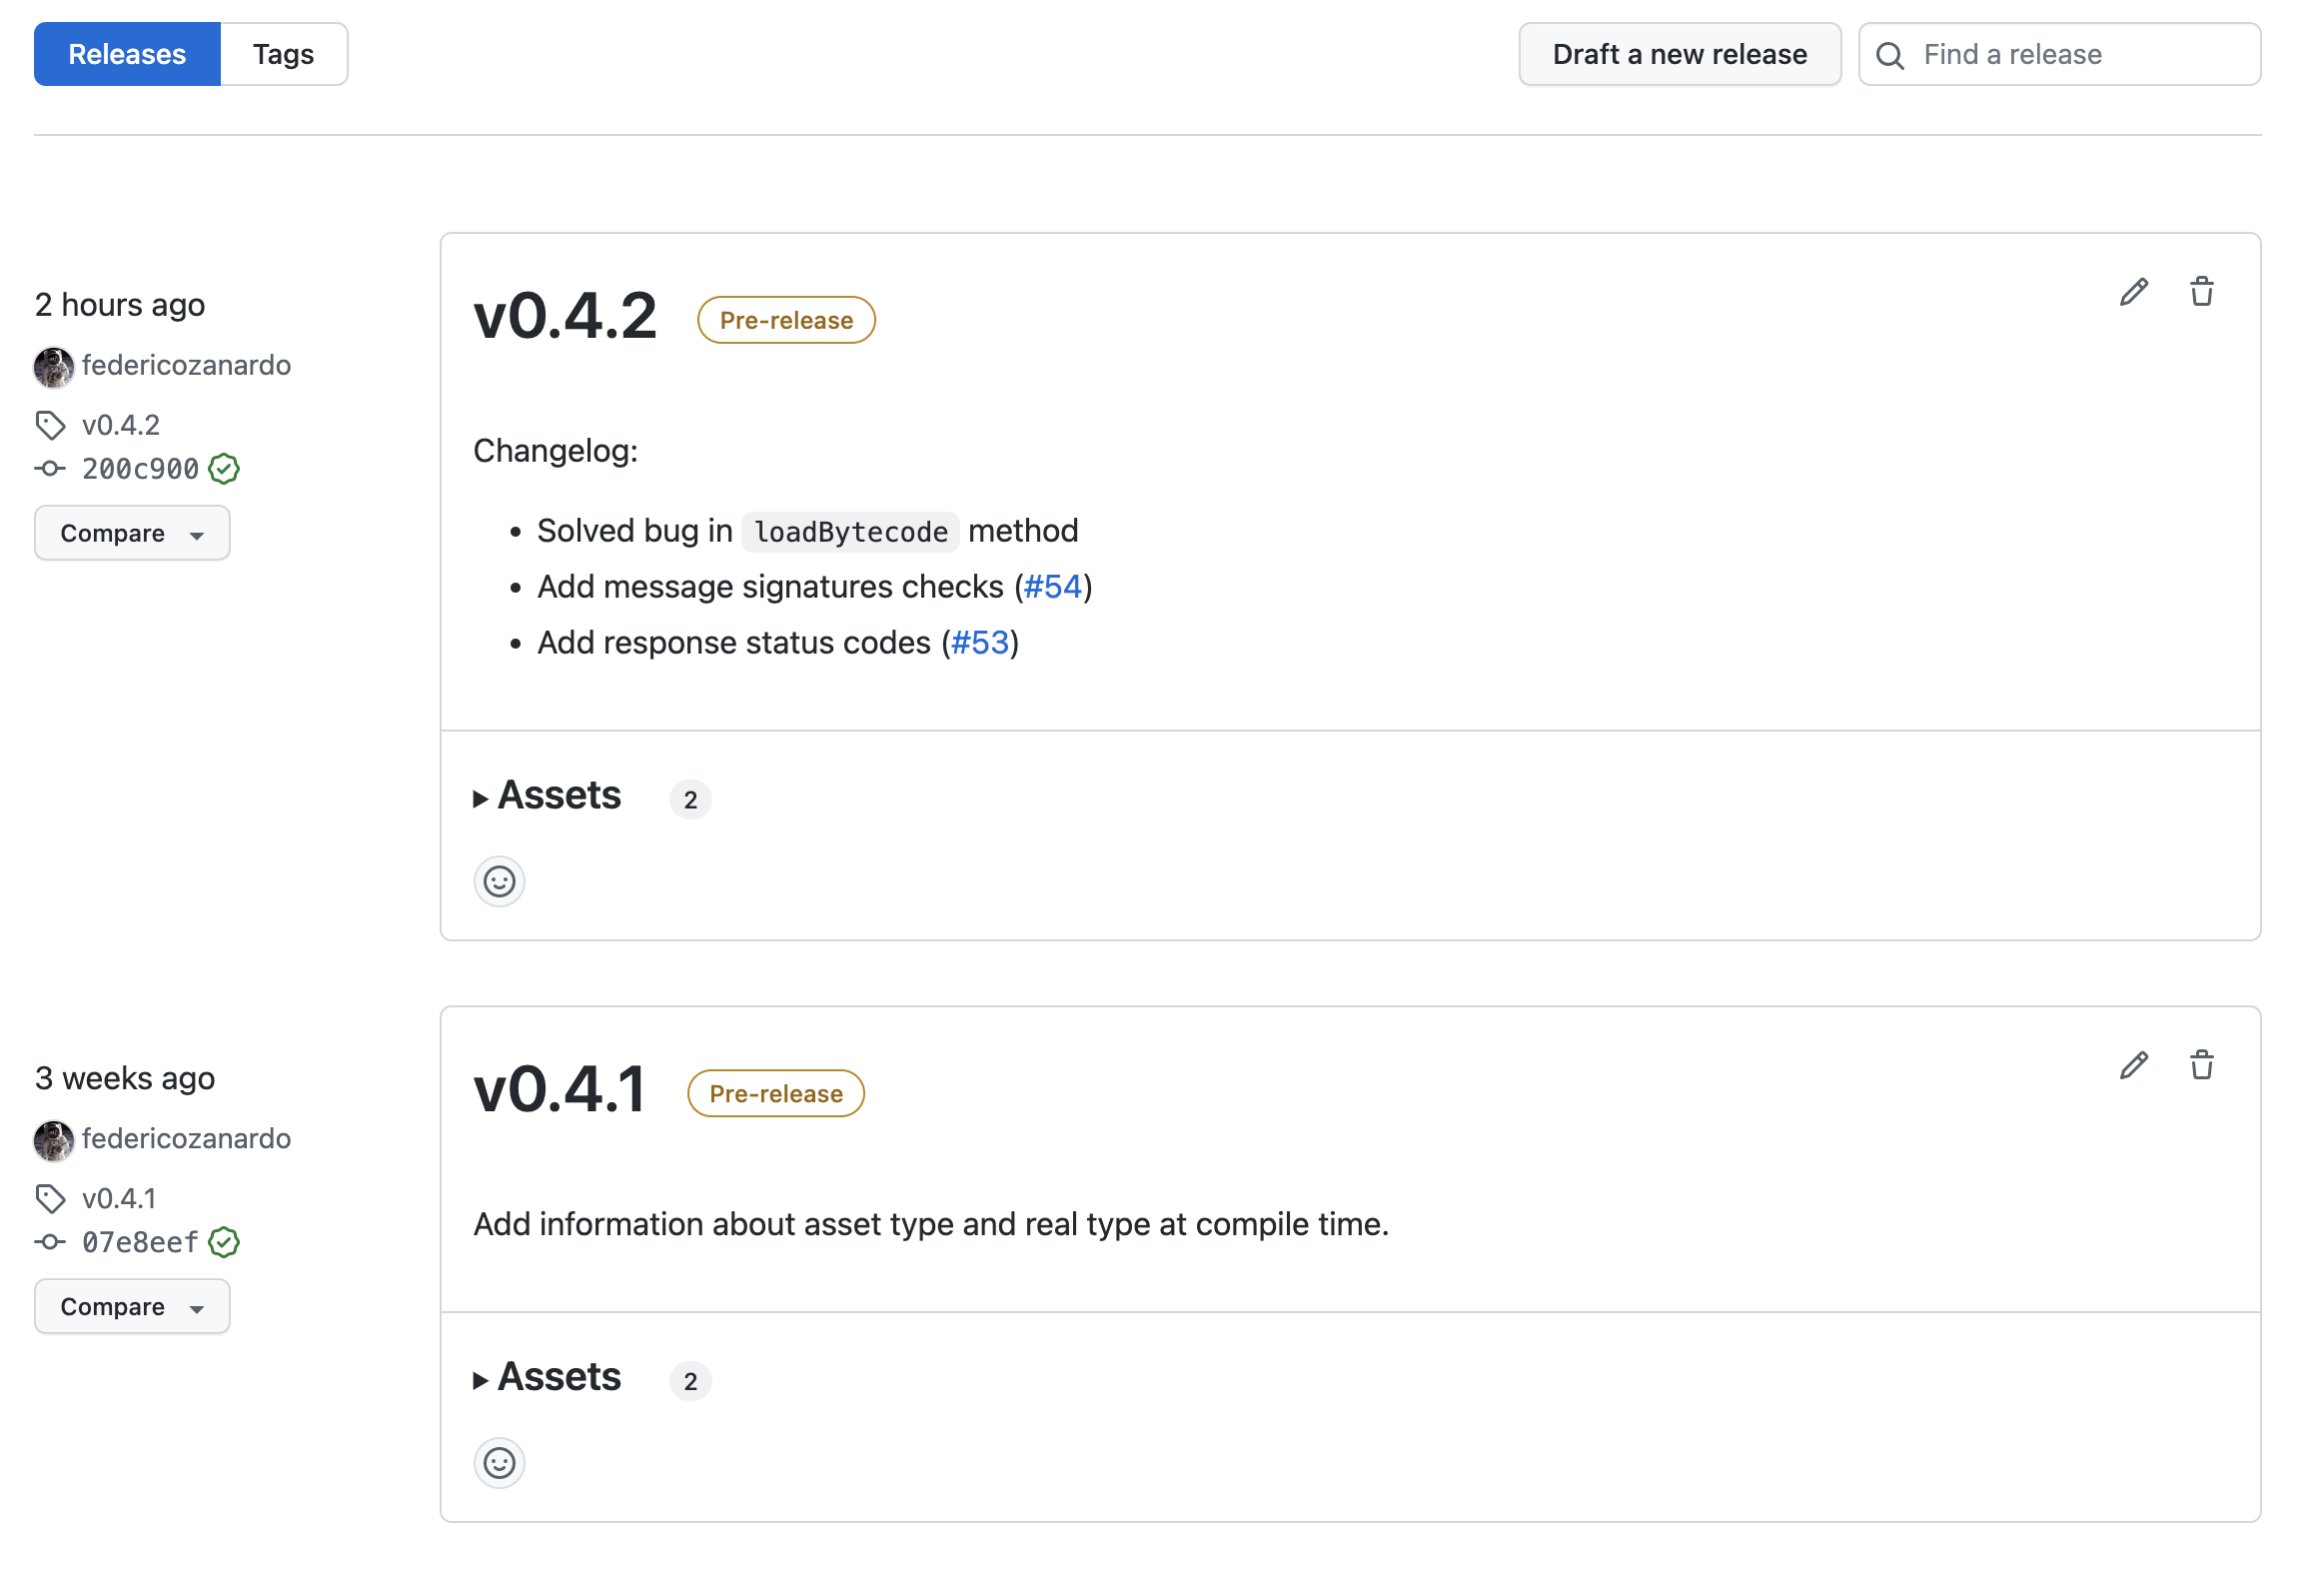
\includegraphics[width=0.9\textwidth]{immagini/capitolo-5/releases.png}
		\caption{Various project releases. For each release it is possible to download the code and start an 
    instance of \textit{Stipula}.}
		\label{fig:releases}
	\end{center}
\end{figure}

\begin{figure}[htbp]
	\begin{center}
		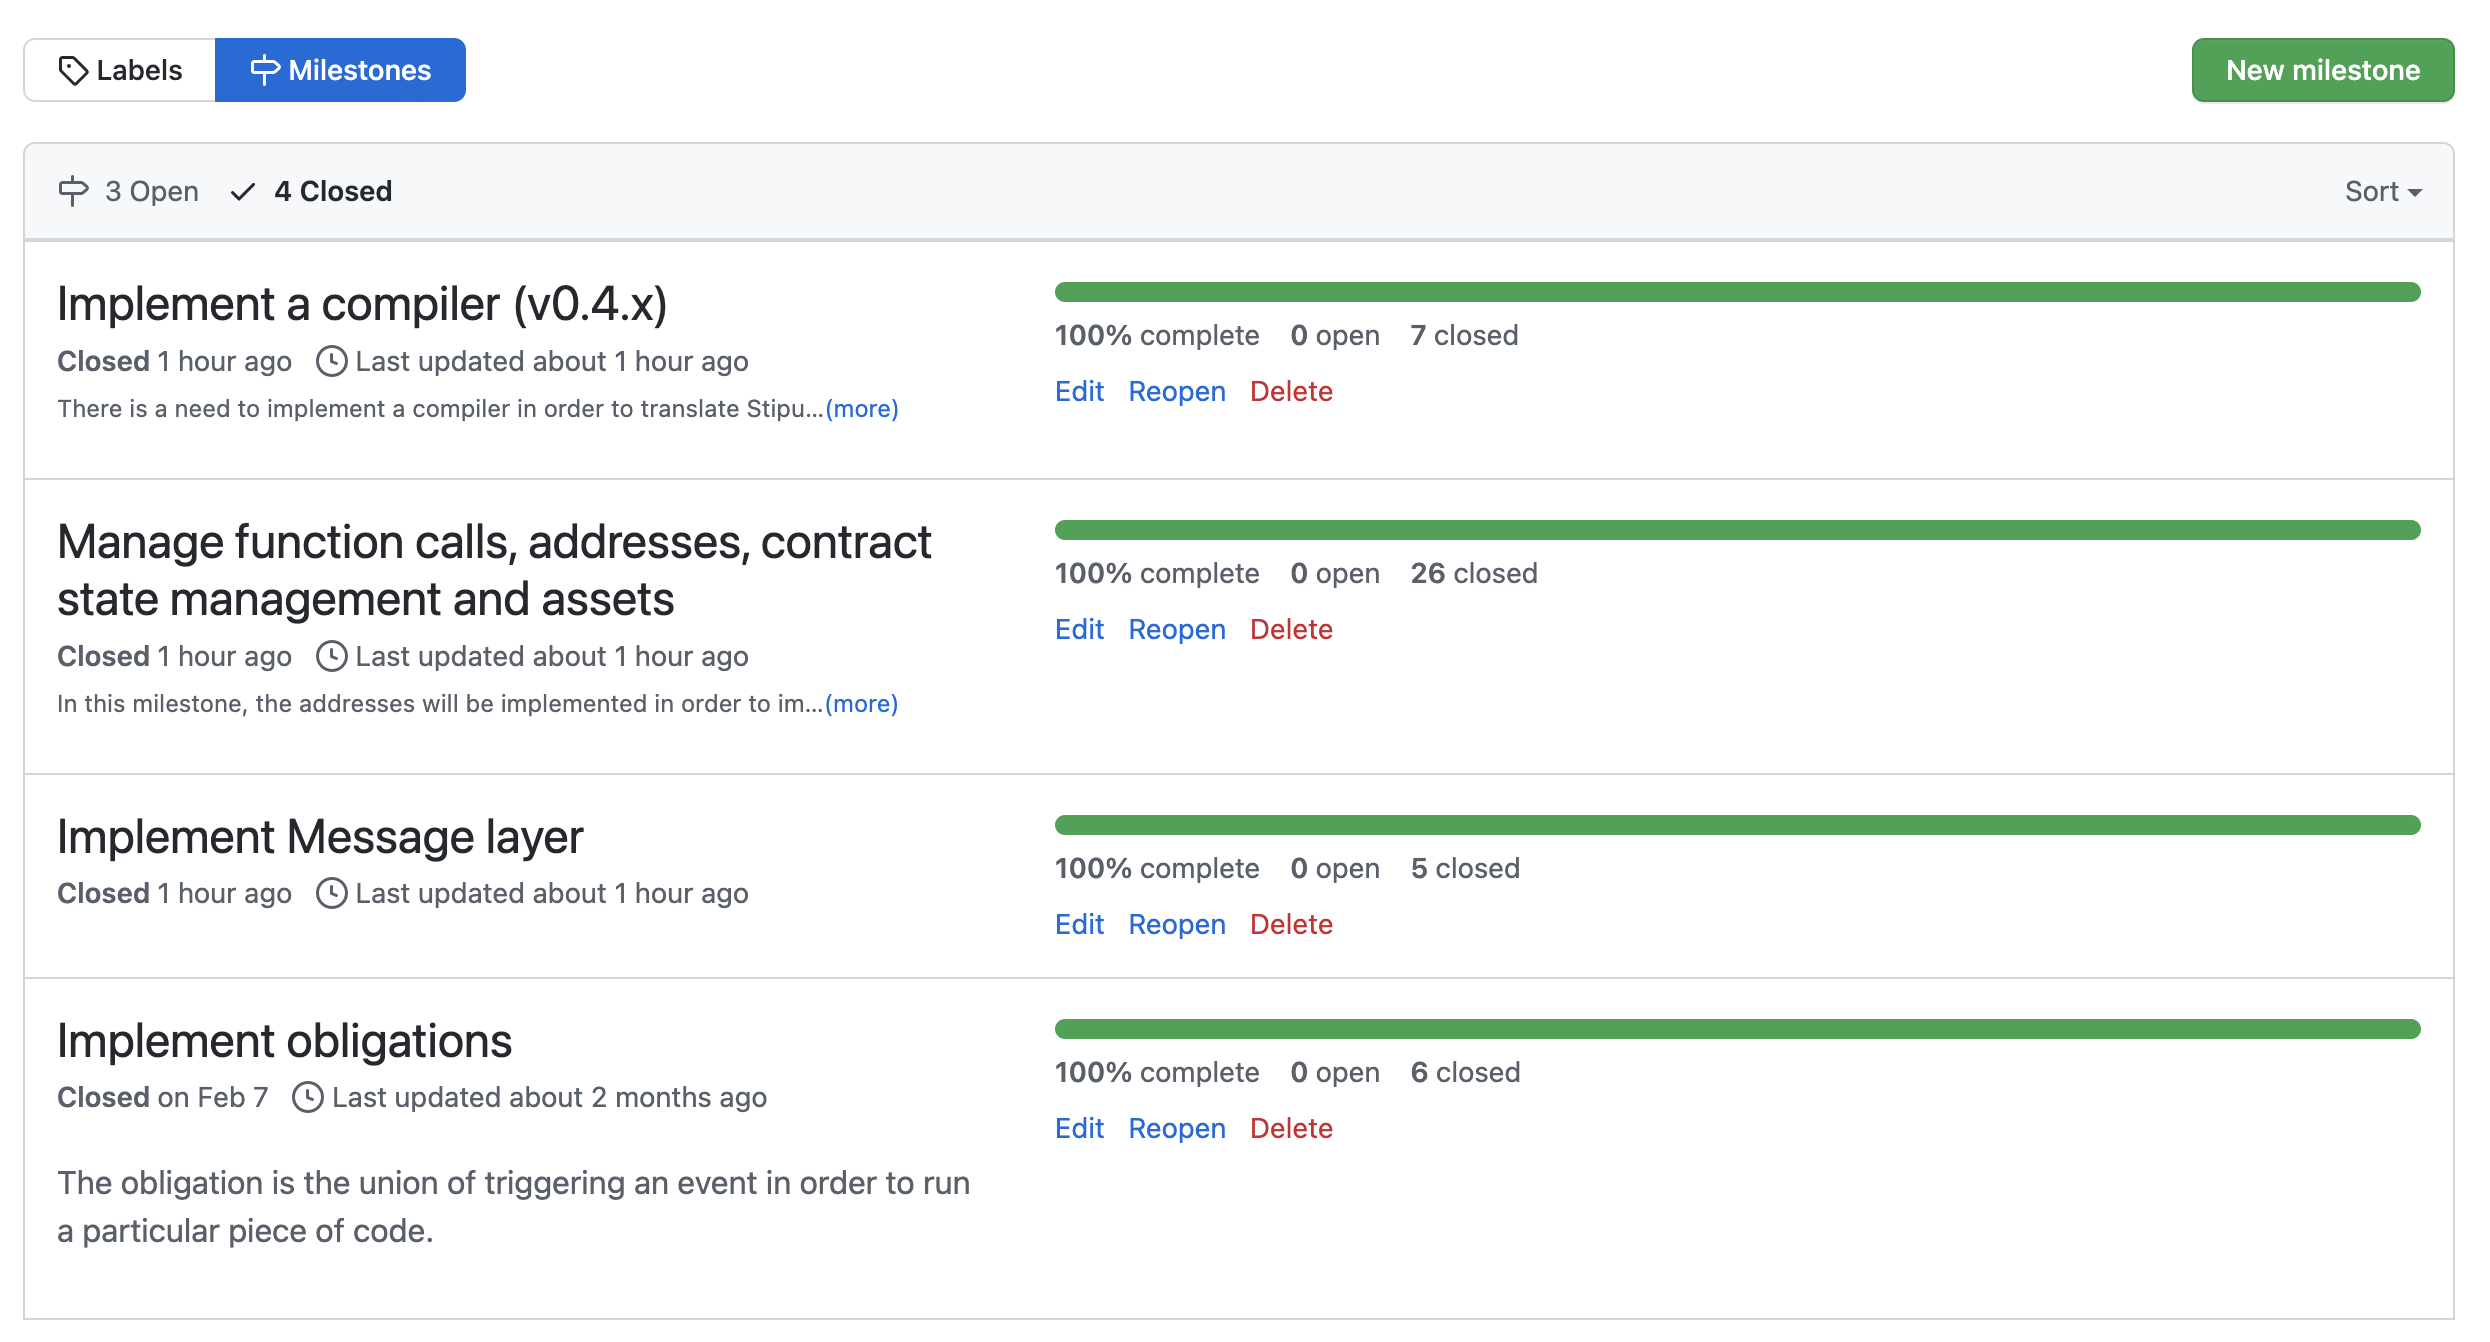
\includegraphics[width=0.9\textwidth]{immagini/capitolo-5/milestones-closed.png}
		\caption{Milestones completed.}
		\label{fig:milestones-closed}
	\end{center}
\end{figure}

\begin{figure}[htbp]
	\begin{center}
		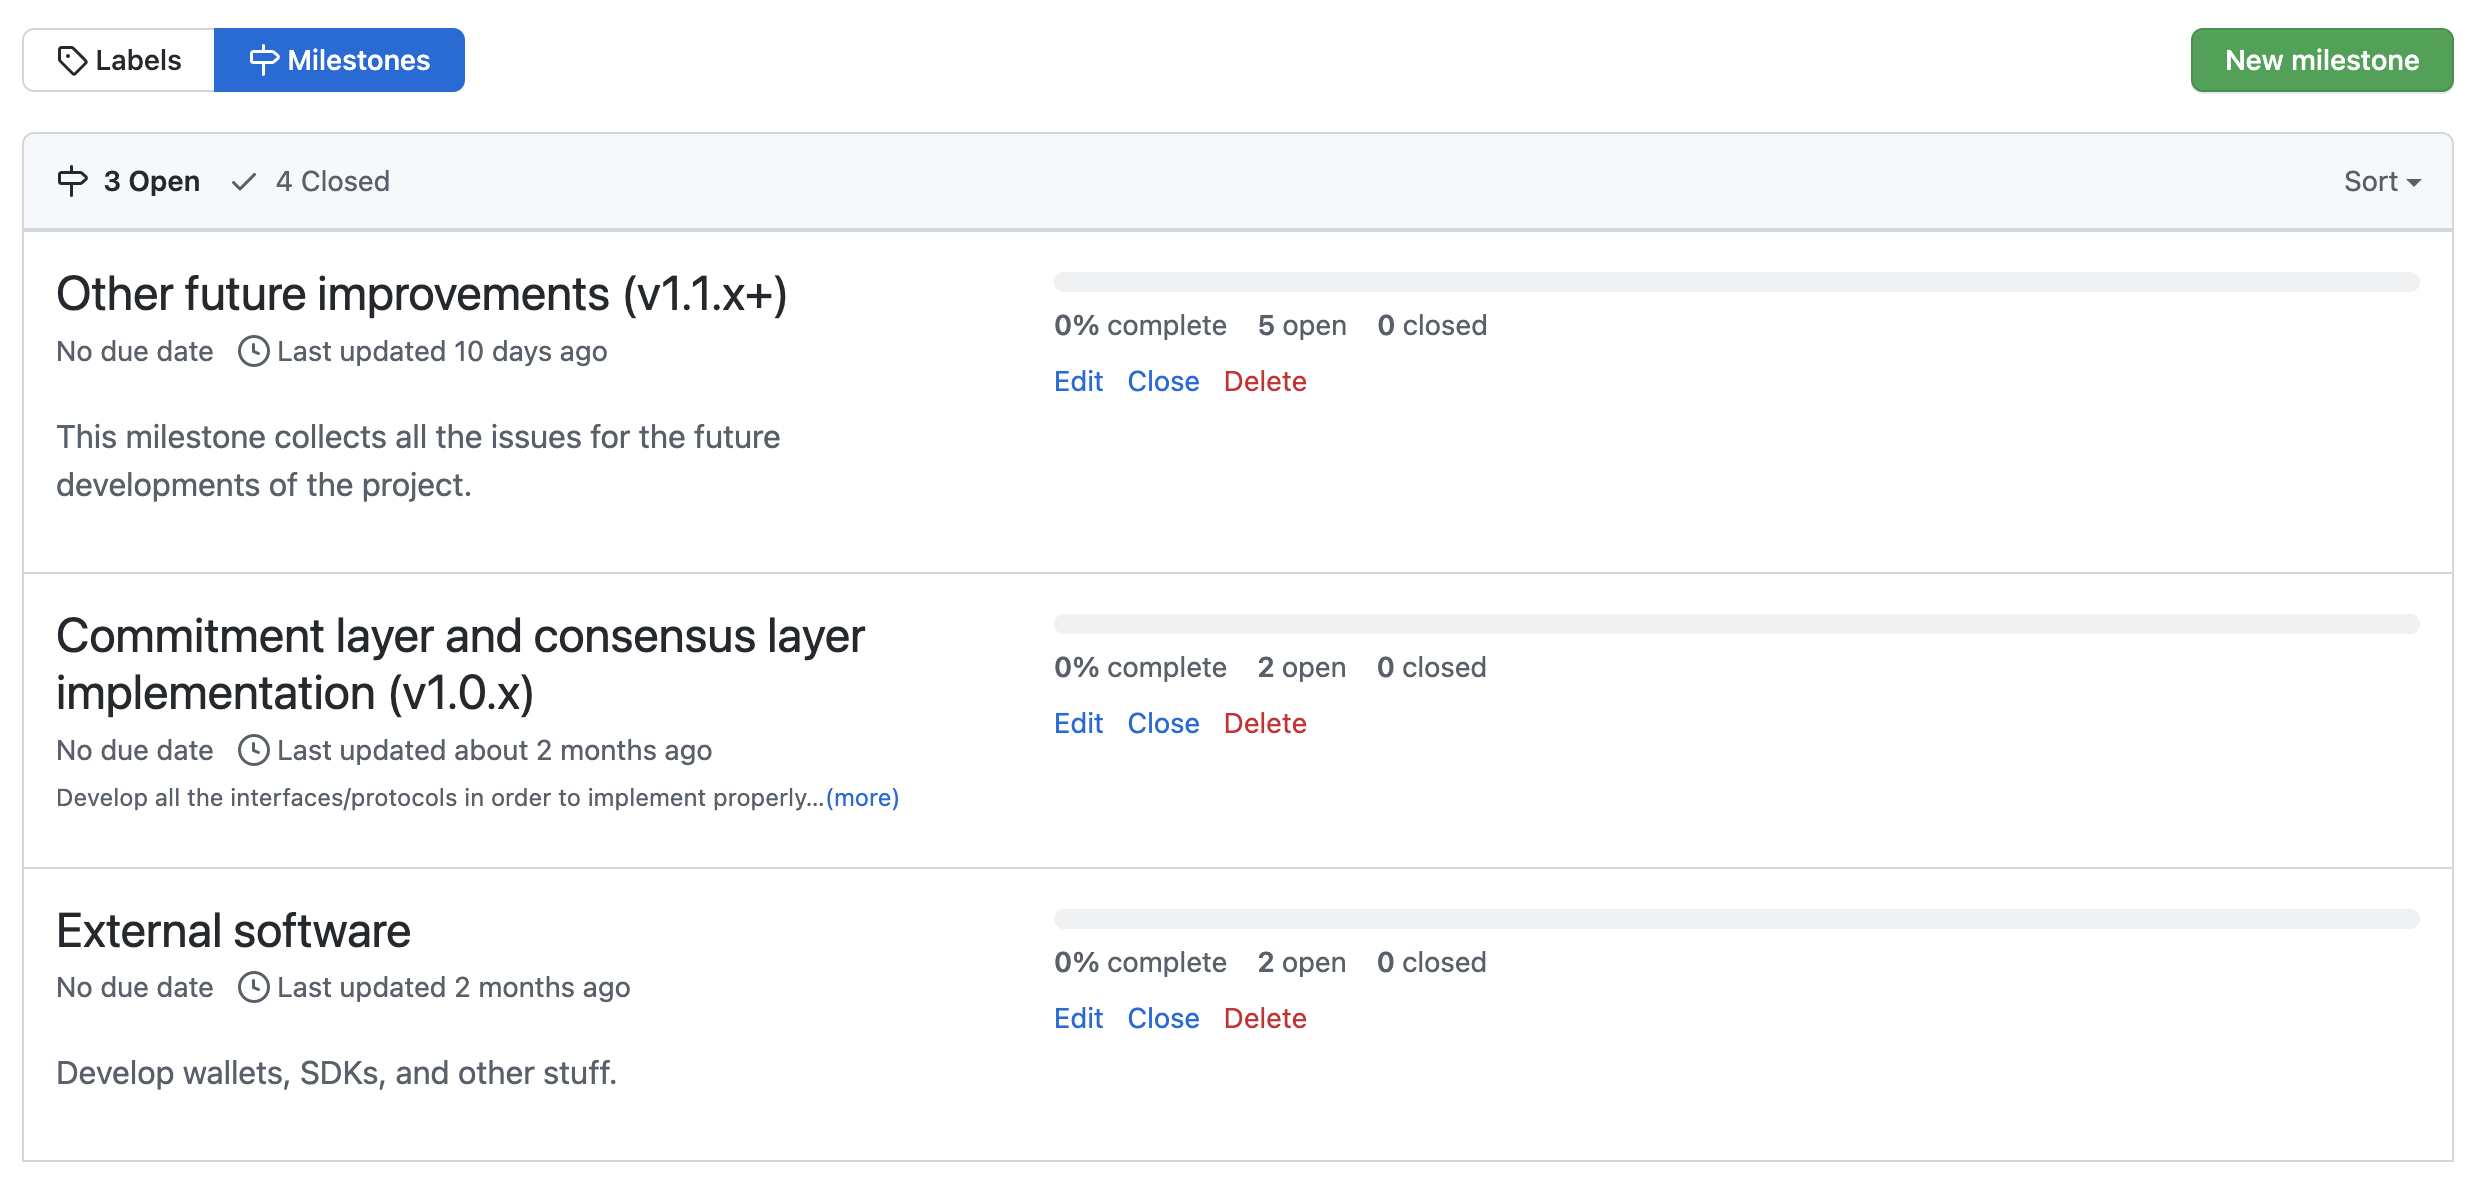
\includegraphics[width=0.9\textwidth]{immagini/capitolo-5/milestones-opened.png}
		\caption{Milestone opened.}
		\label{fig:milestones-opened}
	\end{center}
\end{figure}

\subsection{Installation}

Starting a \textit{Stipula} server can be done by downloading the code and installing all the packages, or 
by downloading a Docker image and running the container. For manual installation, you need:
\begin{enumerate}
  \item Java SDK 8
  \item Gradle 7.6.0
  \item Gson 2.10.1 
  \item LevelDb 0.9
  \item ANTLR 4.10
  \item JUnit 5.8.1
\end{enumerate}

The \ref{app:gradle} appendix contains the code of the \verb|build.gradle| file, which allows you to 
install and manage the project packages.

For a faster and easier to manage installation it is better to use a Docker image. You can create an 
instance of \textit{Stipula} with Docker in two ways:
\begin{enumerate}
  \item Download the project and run \verb|docker build -t stipula-node:<version> .|, where you must 
  specify the version you want to use instead of \verb|<version>|. You also specify the version in the 
  \verb|docker-compose.yml| file and execute the command \verb|docker-compose -f docker-compose.yml up -d|;
  \item Download the Docker files and specify in the \verb|docker-compose.yml| file that the image you 
  want to use must be downloaded from a particular page \autocite{site:stipula-github-available-packages}, 
  that is, \verb|image: "ghcr.io/federicozanardo/stipula-node:<version>"|. To start the container, use 
  the command \verb|docker-compose -f docker-compose.yml up -d|.
\end{enumerate}

The benefit you get is that you can run an instance on any machine that supports Docker and takes the 
responsibility off managing package updates.

Furthermore, each Docker image available at the address 
\begin{Verbatim}
  ghcr.io/federicozanardo/stipula-node:<version>
\end{Verbatim}
is an image that is created at each new release, to which it is obviously subjected to tests. In the 
appendix \ref{app:docker} there is the code of the \verb|Dockerfile| and \verb|docker-compose.yml|.

\label{database-seeding}
Due to the limitations of the implemented architecture, to carry out tests and demonstrate the 
functioning of the implemented implementation, there is the need to initialize assets and 
single-use-seals for addresses. To do this, it is necessary to set the \verb|SEED| environment variable: 
by setting \verb|yes|, assets and single-use-seals will be created when the program is started; valuing 
with \verb|no|, this procedure will not be performed. The enhancement of this environment variable can be 
done inside the \verb|docker-compose.yml| (line 12). The following chapter will illustrate the limits of 
this architecture and propose solutions. In the future, this database \textit{seeding} procedure will be 
removed.
